\documentclass[twoside]{book}

% Packages required by doxygen
\usepackage{fixltx2e}
\usepackage{calc}
\usepackage{doxygen}
\usepackage[export]{adjustbox} % also loads graphicx
\usepackage{graphicx}
\usepackage[utf8]{inputenc}
\usepackage{makeidx}
\usepackage{multicol}
\usepackage{multirow}
\PassOptionsToPackage{warn}{textcomp}
\usepackage{textcomp}
\usepackage[nointegrals]{wasysym}
\usepackage[table]{xcolor}

% Font selection
\usepackage[T1]{fontenc}
\usepackage[scaled=.90]{helvet}
\usepackage{courier}
\usepackage{amssymb}
\usepackage{sectsty}
\renewcommand{\familydefault}{\sfdefault}
\allsectionsfont{%
  \fontseries{bc}\selectfont%
  \color{darkgray}%
}
\renewcommand{\DoxyLabelFont}{%
  \fontseries{bc}\selectfont%
  \color{darkgray}%
}
\newcommand{\+}{\discretionary{\mbox{\scriptsize$\hookleftarrow$}}{}{}}

% Page & text layout
\usepackage{geometry}
\geometry{%
  a4paper,%
  top=2.5cm,%
  bottom=2.5cm,%
  left=2.5cm,%
  right=2.5cm%
}
\tolerance=750
\hfuzz=15pt
\hbadness=750
\setlength{\emergencystretch}{15pt}
\setlength{\parindent}{0cm}
\setlength{\parskip}{3ex plus 2ex minus 2ex}
\makeatletter
\renewcommand{\paragraph}{%
  \@startsection{paragraph}{4}{0ex}{-1.0ex}{1.0ex}{%
    \normalfont\normalsize\bfseries\SS@parafont%
  }%
}
\renewcommand{\subparagraph}{%
  \@startsection{subparagraph}{5}{0ex}{-1.0ex}{1.0ex}{%
    \normalfont\normalsize\bfseries\SS@subparafont%
  }%
}
\makeatother

% Headers & footers
\usepackage{fancyhdr}
\pagestyle{fancyplain}
\fancyhead[LE]{\fancyplain{}{\bfseries\thepage}}
\fancyhead[CE]{\fancyplain{}{}}
\fancyhead[RE]{\fancyplain{}{\bfseries\leftmark}}
\fancyhead[LO]{\fancyplain{}{\bfseries\rightmark}}
\fancyhead[CO]{\fancyplain{}{}}
\fancyhead[RO]{\fancyplain{}{\bfseries\thepage}}
\fancyfoot[LE]{\fancyplain{}{}}
\fancyfoot[CE]{\fancyplain{}{}}
\fancyfoot[RE]{\fancyplain{}{\bfseries\scriptsize Generated by Doxygen }}
\fancyfoot[LO]{\fancyplain{}{\bfseries\scriptsize Generated by Doxygen }}
\fancyfoot[CO]{\fancyplain{}{}}
\fancyfoot[RO]{\fancyplain{}{}}
\renewcommand{\footrulewidth}{0.4pt}
\renewcommand{\chaptermark}[1]{%
  \markboth{#1}{}%
}
\renewcommand{\sectionmark}[1]{%
  \markright{\thesection\ #1}%
}

% Indices & bibliography
\usepackage{natbib}
\usepackage[titles]{tocloft}
\setcounter{tocdepth}{3}
\setcounter{secnumdepth}{5}
\makeindex

% Hyperlinks (required, but should be loaded last)
\usepackage{ifpdf}
\ifpdf
  \usepackage[pdftex,pagebackref=true]{hyperref}
\else
  \usepackage[ps2pdf,pagebackref=true]{hyperref}
\fi
\hypersetup{%
  colorlinks=true,%
  linkcolor=blue,%
  citecolor=blue,%
  unicode%
}

% Custom commands
\newcommand{\clearemptydoublepage}{%
  \newpage{\pagestyle{empty}\cleardoublepage}%
}

\usepackage{caption}
\captionsetup{labelsep=space,justification=centering,font={bf},singlelinecheck=off,skip=4pt,position=top}

%===== C O N T E N T S =====

\begin{document}

% Titlepage & ToC
\pagenumbering{alph}
\begin{titlepage}
\vspace*{7cm}
\begin{center}%
{\Large superquadric-\/model }\\
\vspace*{1cm}
{\large Generated by Doxygen 1.8.14}\\
\end{center}
\end{titlepage}
\clearemptydoublepage
\pagenumbering{roman}
\tableofcontents
\clearemptydoublepage
\pagenumbering{arabic}

%--- Begin generated contents ---
\chapter{Module Index}
\section{Modules}
Here is a list of all modules\+:\begin{DoxyCompactList}
\item \contentsline{section}{superquadric-\/model}{\pageref{group__superquadric-model}}{}
\end{DoxyCompactList}

\chapter{Hierarchical Index}
\section{Class Hierarchy}
This inheritance list is sorted roughly, but not completely, alphabetically\+:\begin{DoxyCompactList}
\item \contentsline{section}{Spatial\+Density\+Filter}{\pageref{classSpatialDensityFilter}}{}
\item \contentsline{section}{Superq\+Computation}{\pageref{classSuperqComputation}}{}
\item \contentsline{section}{Super\+Quadric\+\_\+\+N\+LP}{\pageref{classSuperQuadric__NLP}}{}
\item \contentsline{section}{superquadric\+Model\+\_\+\+I\+DL}{\pageref{classsuperquadricModel__IDL}}{}
\begin{DoxyCompactList}
\item \contentsline{section}{Superq\+Module}{\pageref{classSuperqModule}}{}
\end{DoxyCompactList}
\item \contentsline{section}{Superq\+Visualization}{\pageref{classSuperqVisualization}}{}
\end{DoxyCompactList}

\chapter{Data Structure Index}
\section{Data Structures}
Here are the data structures with brief descriptions\+:\begin{DoxyCompactList}
\item\contentsline{section}{\mbox{\hyperlink{classSpatialDensityFilter}{Spatial\+Density\+Filter}} \\*This class filters the point cloud according to its density }{\pageref{classSpatialDensityFilter}}{}
\item\contentsline{section}{\mbox{\hyperlink{classSuperqComputation}{Superq\+Computation}} \\*This class provides a thread for computing in real time the superquadric, filtering the point cloud and the superquadric }{\pageref{classSuperqComputation}}{}
\item\contentsline{section}{\mbox{\hyperlink{classSuperqModule}{Superq\+Module}} \\*Handle the superquadric computation and visualization, the point cloud and superquadric filtering and the interaction with the user }{\pageref{classSuperqModule}}{}
\item\contentsline{section}{\mbox{\hyperlink{classSuperQuadric__NLP}{Super\+Quadric\+\_\+\+N\+LP}} \\*This class solves the optimization problem with the Ipopt software package and returns the estiamted superquadric, better fitting a given point cloud }{\pageref{classSuperQuadric__NLP}}{}
\item\contentsline{section}{\mbox{\hyperlink{classsuperquadricModel__IDL}{superquadric\+Model\+\_\+\+I\+DL}} \\*Superquadric\+Model\+\_\+\+I\+DL I\+DL Interface to \mbox{\hyperlink{group__superquadric-model}{superquadric-\/model}} services }{\pageref{classsuperquadricModel__IDL}}{}
\item\contentsline{section}{\mbox{\hyperlink{classSuperqVisualization}{Superq\+Visualization}} \\*This class shows the point cloud used for modeling or the estimated superquadric overlapped on the camera image and in real time }{\pageref{classSuperqVisualization}}{}
\end{DoxyCompactList}

\chapter{Module Documentation}
\section{superquadric-\/model}
\label{group__superquadric-model}\index{superquadric-\/model@{superquadric-\/model}}


~\newline
 Framework for object detecting and modeling.  


~\newline
 Framework for object detecting and modeling. 

Version\+:1.\+0 \begin{DoxyAuthor}{Author}
Giulia Vezzani \href{mailto:giulia.vezzani@iit.it}{\tt giulia.\+vezzani@iit.\+it} ~\newline
 
\end{DoxyAuthor}
\begin{DoxyCopyright}{Copyright}
Released under the terms of the G\+NU G\+PL v2.\+0 
\end{DoxyCopyright}
\hypertarget{group__superquadric-model_intro_sec}{}\subsection{Description}\label{group__superquadric-model_intro_sec}
This module provides an object modeling tool based on superquadric functions. A tutorial on how to use the module is provided in the dedicated repository \href{https://github.com/robotology/superquadric-model/tree/master/tutorial}{\tt {\bfseries tutorial}}.

This page illustrates the main parameters of the module (Section {\bfseries Parameters}), the available ports and services. The modules parameters are labeled as standard and advanced. Note\+: change the advanced parameters only if you are familiar with the implemented techniques.

The module can also provides {\bfseries three output files} is the saving options is enabled\+:
\begin{DoxyItemize}
\item {\bfseries tag-\/file.\+txt} or {\bfseries output.\+txt} (if the point cloud is given through a file or a seed point), containing the reconstructed superquadric and some information about I\+P\+O\+PT algorithm;
\item {\bfseries S\+F\+M-\/tag-\/file.\+off} containing the 3D points coming from S\+FM;
\item {\bfseries filtered-\/tag-\/file.\+off} containing the filtered 3D points (if filtering is enabled).
\end{DoxyItemize}\hypertarget{group__superquadric-model_parameters_sec}{}\subsection{Parameters}\label{group__superquadric-model_parameters_sec}
~\newline

\begin{DoxyItemize}
\item --context\+: Select the current context (standard parameter).
\item --from\+: Configuration file name (standard parameter).
\item --tag\+\_\+file\+: Tag for saving files (standard parameter).
\item --visualization\+\_\+on\+: Variable to enable or not the visualization (standard parameter -\/ thrift service available).
\item --camera\+: Eye used for projection of the 3D points on the superquadric surface to the 2D pixels (standard parameter -\/ thrift service available).
\item --vis\+\_\+points\+: Number of points used for visualization (standard parameter -\/ thrift service available).
\item --what\+\_\+to\+\_\+plot\+: What to plot among the estimated superquadric and the acquired 3D points (standard parameter -\/ thrift service available).
\item --tol\+: Desired convergence tolerance (relative). Determines the convergence tolerance for the I\+P\+O\+PT algorithm (standard parameter -\/ thrift service available).
\item --acceptable\+\_\+iter\+: I\+P\+O\+PT acceptable iter. Number of acceptable iterates before triggering termination. If the algorithm encounters this many successive acceptable iterates, it terminates, assuming that the problem has been solved to best possible accuracy given round-\/off. If it is set to zero, this heuristic is disabled (advanced parameter-\/ thrift service available).
\item --max\+\_\+iter\+: I\+P\+O\+PT maximum iteration (advanced parameter-\/ thrift service available).
\item --max\+\_\+cpu\+\_\+time\+: Maximum cpu time for I\+P\+O\+PT algorithm execution (advanced parameter -\/ thrift service available).
\item --mu\+\_\+strategy\+: I\+P\+O\+PT update strategy for barrier parameter. Determines which barrier parameter update strategy is to be used. P\+Ossible values\+: monotone or adaptive (advanced parameter-\/ thrift service available).
\item --nlp\+\_\+scaling\+\_\+method\+: I\+P\+O\+PT nlp\+\_\+scaling\+\_\+method\+: Select the technique used for scaling the problem. Possible values\+: none, user-\/scaling, gradient-\/based, equilibration-\/based (advanced parameter-\/ thrift service available).
\item --filter\+\_\+points\+: Variable to decide to filter points or not (standard parameter -\/ thrift service available).
\item --radius\+: K\+NN radius value for filtering (advanced parameter -\/ thrift service available).
\item --nn\+Threshold\+: K\+KN threshold value for filtering (advanced parameter -\/ thrift service available).
\item --filter\+\_\+superq\+: Variable to decide to filter superq or not (standard parameter -\/ thrift service available).
\item --fixed\+\_\+window\+: Variable to decide if to use a fixed window for the median filter on superquadrics (standard parameter -\/ thrift service available).
\item --median\+\_\+order\+: Window width in case and adaptive window is not used (advanced parameter -\/ thrift service available).
\item --min\+\_\+median\+\_\+order\+: Min window width in case an adaptive window is used (advanced parameter -\/ thrift service available).
\item --max\+\_\+median\+\_\+order\+: Max window width in case an adaptive window is used (advanced parameter -\/ thrift service available). 
\end{DoxyItemize}\hypertarget{group__superquadric-model_inputports_sec}{}\subsection{Input Ports}\label{group__superquadric-model_inputports_sec}

\begin{DoxyItemize}
\item /superquadric-\/model/img\+:i \mbox{[}yarp\+::sig\+::\+Image\+Of\+Pixel\+Rgb\mbox{]} \mbox{[}default carrier\+:tcp\mbox{]}\+: receive the image from the left camera.
\item /superquadric-\/model/point\+:i \mbox{[}yarp\+::os\+::\+Bottle\mbox{]} \mbox{[}default carrier\+:tcp\mbox{]}\+: receive the 2D blob of the object.
\end{DoxyItemize}\hypertarget{group__superquadric-model_outputports_sec}{}\subsection{Output Ports}\label{group__superquadric-model_outputports_sec}

\begin{DoxyItemize}
\item /superquadric-\/model/img\+:o \mbox{[}yarp\+::sig\+::\+Image\+Of\+Pixel\+Mono\mbox{]} \mbox{[}default carrier\+:tcp\mbox{]}\+: send the image from the left camera with the visualized superquadric or points.
\item /superquadric-\/model/superq\+:o \mbox{[}yarp\+::os\+::\+Property\mbox{]} \mbox{[}default carrier\+:tcp\mbox{]}\+: send the estimated superquadric in streaming.
\end{DoxyItemize}\hypertarget{group__superquadric-model_services_sec}{}\subsection{Services}\label{group__superquadric-model_services_sec}

\begin{DoxyItemize}
\item /superquadric-\/model/rpc \mbox{[}rpc-\/server\mbox{]}\+: service port . This service is described in \mbox{\hyperlink{classsuperquadricModel__IDL}{superquadric\+Model\+\_\+\+I\+DL}} (idl.\+thrift) 
\end{DoxyItemize}
\chapter{Data Structure Documentation}
\section{Spatial\+Density\+Filter Class Reference}
\label{classSpatialDensityFilter}\index{Spatial\+Density\+Filter@{Spatial\+Density\+Filter}}


This class filters the point cloud according to its density.  




{\ttfamily \#include $<$superq\+Computation.\+h$>$}

\subsection*{Static Public Member Functions}
\begin{DoxyCompactItemize}
\item 
\mbox{\label{classSpatialDensityFilter_a85931f42a6e96af8c7f331fbd01c15bf}} 
static std\+::vector$<$ int $>$ {\bfseries filter} (const cv\+::\+Mat \&data, const double radius, const int max\+Results, std\+::deque$<$ yarp\+::sig\+::\+Vector $>$ \&points)
\end{DoxyCompactItemize}


\subsection{Detailed Description}
This class filters the point cloud according to its density. 

Definition at line 34 of file superq\+Computation.\+h.



The documentation for this class was generated from the following files\+:\begin{DoxyCompactItemize}
\item 
C\+:/\+Users/upattacini/\+Desktop/superquadric-\/model/include/superq\+Computation.\+h\item 
C\+:/\+Users/upattacini/\+Desktop/superquadric-\/model/src/superq\+Computation.\+cpp\end{DoxyCompactItemize}

\section{Superq\+Computation Class Reference}
\label{classSuperqComputation}\index{Superq\+Computation@{Superq\+Computation}}


This class provides a thread for computing in real time the superquadric, filtering the point cloud and the superquadric.  




{\ttfamily \#include $<$superq\+Computation.\+h$>$}



Inherits Thread.

\subsection*{Public Member Functions}
\begin{DoxyCompactItemize}
\item 
\mbox{\label{classSuperqComputation_a9ded9044e1c7fe17a70997f27eea7aa7}} 
{\bfseries Superq\+Computation} (yarp\+::os\+::\+Mutex \&mutex\+\_\+shared, int \+\_\+rate, bool \+\_\+filter\+\_\+points, bool \+\_\+filter\+\_\+superq, bool \+\_\+fixed\+\_\+window, std\+::deque$<$ yarp\+::sig\+::\+Vector $>$ \&\+\_\+points, std\+::string \+\_\+tag\+\_\+file, double \+\_\+threshold\+\_\+median, const yarp\+::os\+::\+Property \&filters\+\_\+points\+\_\+par, yarp\+::sig\+::\+Vector \&\+\_\+x, yarp\+::sig\+::\+Vector \&\+\_\+x\+\_\+filtered, const yarp\+::os\+::\+Property \&filters\+\_\+superq\+\_\+par, const yarp\+::os\+::\+Property \&optimizer\+\_\+par, const std\+::string \&\+\_\+home\+Context\+Path, bool \+\_\+save\+\_\+points, yarp\+::os\+::\+Resource\+Finder $\ast$rf)
\item 
void \mbox{\hyperlink{classSuperqComputation_a4f841a006336a06d0a349f8a57707524}{set\+Points\+Filter\+Par}} (const yarp\+::os\+::\+Property \&new\+Options, bool first\+\_\+time)
\begin{DoxyCompactList}\small\item\em Set options for filtering the point cloud. \end{DoxyCompactList}\item 
void \mbox{\hyperlink{classSuperqComputation_ac0eb6516ba435573f74b03ed4177d8d0}{set\+Superq\+Filter\+Par}} (const yarp\+::os\+::\+Property \&new\+Options, bool first\+\_\+time)
\begin{DoxyCompactList}\small\item\em Set options for filtering the superquadric. \end{DoxyCompactList}\item 
void \mbox{\hyperlink{classSuperqComputation_afa65ce67fb294f38c4e843540f96de3c}{set\+Ipopt\+Par}} (const yarp\+::os\+::\+Property \&new\+Options, bool first\+\_\+time)
\begin{DoxyCompactList}\small\item\em Set options for the optimization problem solved by Ipopt. \end{DoxyCompactList}\item 
yarp\+::os\+::\+Property \mbox{\hyperlink{classSuperqComputation_a110d429be796961d8c4fe8ce9b944362}{get\+Points\+Filter\+Par}} ()
\begin{DoxyCompactList}\small\item\em Get options used for filtering the point cloud. \end{DoxyCompactList}\item 
yarp\+::os\+::\+Property \mbox{\hyperlink{classSuperqComputation_a1f93a7688ef418d2ca9402cff5621048}{get\+Superq\+Filter\+Par}} ()
\begin{DoxyCompactList}\small\item\em Get options used for filtering the superquadric. \end{DoxyCompactList}\item 
yarp\+::os\+::\+Property \mbox{\hyperlink{classSuperqComputation_a1d95dee395edafac26144758f3bd5830}{get\+Ipopt\+Par}} ()
\begin{DoxyCompactList}\small\item\em Get options used for solving the optimization problem with Ipopt. \end{DoxyCompactList}\item 
void \mbox{\hyperlink{classSuperqComputation_a1780009371c09327b8491189dee66b20}{set\+Par}} (const std\+::string \&par\+\_\+name, const std\+::string \&value)
\begin{DoxyCompactList}\small\item\em Set a parameter equal to a value. \end{DoxyCompactList}\item 
\mbox{\label{classSuperqComputation_ada608220b124f8ffcf458d93bad4f227}} 
virtual bool \mbox{\hyperlink{classSuperqComputation_ada608220b124f8ffcf458d93bad4f227}{thread\+Init}} ()
\begin{DoxyCompactList}\small\item\em Init function of Thread class. \end{DoxyCompactList}\item 
\mbox{\label{classSuperqComputation_a4a4ac55200a7633a2384da0f0d945ba9}} 
virtual void \mbox{\hyperlink{classSuperqComputation_a4a4ac55200a7633a2384da0f0d945ba9}{run}} ()
\begin{DoxyCompactList}\small\item\em Run function of Thread class. \end{DoxyCompactList}\item 
\mbox{\label{classSuperqComputation_a9e9646fce399266221fb87bc1e1c2476}} 
virtual void \mbox{\hyperlink{classSuperqComputation_a9e9646fce399266221fb87bc1e1c2476}{thread\+Release}} ()
\begin{DoxyCompactList}\small\item\em Release function of Thread class. \end{DoxyCompactList}\item 
void \mbox{\hyperlink{classSuperqComputation_ab8912bb805cf979007985ffb553d43b0}{save\+Points}} (const std\+::string \&namefile, const yarp\+::sig\+::\+Vector \&colors)
\begin{DoxyCompactList}\small\item\em Save point cloud used for reconstructing the superquadric. \end{DoxyCompactList}\item 
\mbox{\label{classSuperqComputation_a39716be08b79ce6ff2ebcb5818fac75e}} 
bool \mbox{\hyperlink{classSuperqComputation_a39716be08b79ce6ff2ebcb5818fac75e}{read\+Point\+Cloud}} ()
\begin{DoxyCompactList}\small\item\em Read the object point cloud from txt for offline tests. \end{DoxyCompactList}\item 
\mbox{\label{classSuperqComputation_a33f9e5ffc074bcf0235d2f49190a60c3}} 
void \mbox{\hyperlink{classSuperqComputation_a33f9e5ffc074bcf0235d2f49190a60c3}{filter}} ()
\begin{DoxyCompactList}\small\item\em Filter the received point cloud. \end{DoxyCompactList}\item 
bool \mbox{\hyperlink{classSuperqComputation_a99887a4fd19d25a3b1ebf46d63558397}{compute\+Superq}} ()
\begin{DoxyCompactList}\small\item\em Compute the superquadric modeling the object. \end{DoxyCompactList}\item 
\mbox{\label{classSuperqComputation_aaf15f0e8aecc808c945ca4036be8c249}} 
void \mbox{\hyperlink{classSuperqComputation_aaf15f0e8aecc808c945ca4036be8c249}{filter\+Superq}} ()
\begin{DoxyCompactList}\small\item\em Filter the superquadri with the median filter. \end{DoxyCompactList}\item 
\mbox{\label{classSuperqComputation_a49c6ca5d5a0d4f0a9a065e0ad448a3e2}} 
void \mbox{\hyperlink{classSuperqComputation_a49c6ca5d5a0d4f0a9a065e0ad448a3e2}{reset\+Median\+Filter}} ()
\begin{DoxyCompactList}\small\item\em Reset median filter. \end{DoxyCompactList}\item 
\mbox{\label{classSuperqComputation_a8d35478d678ddd1711ca63a7e66a13ac}} 
int \mbox{\hyperlink{classSuperqComputation_a8d35478d678ddd1711ca63a7e66a13ac}{adapt\+Wind\+Computation}} ()
\begin{DoxyCompactList}\small\item\em Compute window size according to the object velocity. \end{DoxyCompactList}\item 
\mbox{\label{classSuperqComputation_a7e3d03f909761bcf7ab70a3eeabcee23}} 
bool \mbox{\hyperlink{classSuperqComputation_a7e3d03f909761bcf7ab70a3eeabcee23}{config\+Filter\+Superq}} ()
\begin{DoxyCompactList}\small\item\em Configure superquadric filter. \end{DoxyCompactList}\item 
\mbox{\label{classSuperqComputation_a5076581260278406719f1df46fa528c7}} 
bool \mbox{\hyperlink{classSuperqComputation_a5076581260278406719f1df46fa528c7}{config3\+Dpoints}} ()
\begin{DoxyCompactList}\small\item\em Configure point cloud filter. \end{DoxyCompactList}\item 
yarp\+::sig\+::\+Vector \mbox{\hyperlink{classSuperqComputation_aa659eda30d49322192be2565f44c0fb9}{get\+Solution}} (bool filtered\+\_\+or\+\_\+not)
\begin{DoxyCompactList}\small\item\em Return the computed superquadric. \end{DoxyCompactList}\item 
void \mbox{\hyperlink{classSuperqComputation_a52c81fde3c749d05572eecd3319ac905}{send\+Points}} (const std\+::deque$<$ yarp\+::sig\+::\+Vector $>$ \&p)
\begin{DoxyCompactList}\small\item\em Get the point cloud for computing the superquadric. \end{DoxyCompactList}\item 
\mbox{\label{classSuperqComputation_a7d81b7930e2c8799dcea18745e574a2a}} 
void \mbox{\hyperlink{classSuperqComputation_a7d81b7930e2c8799dcea18745e574a2a}{get\+Points3D}} ()
\begin{DoxyCompactList}\small\item\em Get the point cloud for computing the superquadric. \end{DoxyCompactList}\item 
double \mbox{\hyperlink{classSuperqComputation_a6822767dea4b3b819f9190289d9f89a5}{get\+Time}} ()
\begin{DoxyCompactList}\small\item\em Return the computation time for estimating the superquadric. \end{DoxyCompactList}\end{DoxyCompactItemize}
\subsection*{Data Fields}
\begin{DoxyCompactItemize}
\item 
\mbox{\label{classSuperqComputation_ab30b0c645ad52b61fe7a947eb3c227ed}} 
int \mbox{\hyperlink{classSuperqComputation_ab30b0c645ad52b61fe7a947eb3c227ed}{std\+\_\+median\+\_\+order}}
\begin{DoxyCompactList}\small\item\em median order width \end{DoxyCompactList}\item 
\mbox{\label{classSuperqComputation_af8ec20c3b393c5f82c6662a0a2c1145d}} 
int \mbox{\hyperlink{classSuperqComputation_af8ec20c3b393c5f82c6662a0a2c1145d}{max\+\_\+median\+\_\+order}}
\begin{DoxyCompactList}\small\item\em max median order width \end{DoxyCompactList}\item 
\mbox{\label{classSuperqComputation_a3973557e78ae06f3f32d6e279585f4ac}} 
yarp\+::sig\+::\+Vector \& \mbox{\hyperlink{classSuperqComputation_a3973557e78ae06f3f32d6e279585f4ac}{x}}
\begin{DoxyCompactList}\small\item\em Object superquadric. \end{DoxyCompactList}\item 
\mbox{\label{classSuperqComputation_a7e297c9aaff44b1c83e2134f17f9d949}} 
yarp\+::sig\+::\+Vector \& \mbox{\hyperlink{classSuperqComputation_a7e297c9aaff44b1c83e2134f17f9d949}{x\+\_\+filtered}}
\begin{DoxyCompactList}\small\item\em Filtered object superquadric. \end{DoxyCompactList}\item 
\mbox{\label{classSuperqComputation_a1d88efa996ff50a62e46bbf4fb8bca0b}} 
std\+::deque$<$ yarp\+::sig\+::\+Vector $>$ \& \mbox{\hyperlink{classSuperqComputation_a1d88efa996ff50a62e46bbf4fb8bca0b}{points}}
\begin{DoxyCompactList}\small\item\em Object point cloud. \end{DoxyCompactList}\item 
\mbox{\label{classSuperqComputation_a4862f75f1f976e449f434bd1d78f8445}} 
std\+::deque$<$ cv\+::\+Point $>$ \mbox{\hyperlink{classSuperqComputation_a4862f75f1f976e449f434bd1d78f8445}{blob\+\_\+points}}
\begin{DoxyCompactList}\small\item\em Object 2D blob. \end{DoxyCompactList}\end{DoxyCompactItemize}
\subsection*{Protected Attributes}
\begin{DoxyCompactItemize}
\item 
\mbox{\label{classSuperqComputation_a2503498f171c08ccba94f754a7554cc3}} 
int \mbox{\hyperlink{classSuperqComputation_a2503498f171c08ccba94f754a7554cc3}{count}}
\begin{DoxyCompactList}\small\item\em Count variable. \end{DoxyCompactList}\item 
\mbox{\label{classSuperqComputation_a61546ef4a16a8daf6a2a92e5fa16eaf5}} 
bool \mbox{\hyperlink{classSuperqComputation_a61546ef4a16a8daf6a2a92e5fa16eaf5}{save\+\_\+points}}
\begin{DoxyCompactList}\small\item\em Boolean variable for enabling point cloud saving. \end{DoxyCompactList}\item 
\mbox{\label{classSuperqComputation_aae8ace8205eac99d97d54f3213bf708b}} 
std\+::string \mbox{\hyperlink{classSuperqComputation_aae8ace8205eac99d97d54f3213bf708b}{tag\+\_\+file}}
\begin{DoxyCompactList}\small\item\em Tag name of files for saving 3D points. \end{DoxyCompactList}\item 
\mbox{\label{classSuperqComputation_a8e71181154ad0c3dfa8d37b2201e290e}} 
std\+::string \mbox{\hyperlink{classSuperqComputation_a8e71181154ad0c3dfa8d37b2201e290e}{home\+Context\+Path}}
\begin{DoxyCompactList}\small\item\em Path where code context is located. \end{DoxyCompactList}\item 
\mbox{\label{classSuperqComputation_a83ea1977c3822c48c917a97068d77f44}} 
yarp\+::os\+::\+Const\+String \mbox{\hyperlink{classSuperqComputation_a83ea1977c3822c48c917a97068d77f44}{point\+Cloud\+File\+Name}}
\begin{DoxyCompactList}\small\item\em Pointcloud name file in case the module runs offline. \end{DoxyCompactList}\item 
\mbox{\label{classSuperqComputation_ab35ce370798ac4744994185539b25a54}} 
std\+::vector$<$ cv\+::\+Point $>$ \mbox{\hyperlink{classSuperqComputation_ab35ce370798ac4744994185539b25a54}{contour}}
\begin{DoxyCompactList}\small\item\em Open\+CV variable for blob extraction. \end{DoxyCompactList}\item 
\mbox{\label{classSuperqComputation_aa8eaa06377f2a937eaafa6a21af2a2d4}} 
yarp\+::os\+::\+Buffered\+Port$<$ yarp\+::os\+::\+Bottle $>$ \mbox{\hyperlink{classSuperqComputation_aa8eaa06377f2a937eaafa6a21af2a2d4}{point\+Port}}
\begin{DoxyCompactList}\small\item\em Port for receiving point cloud. \end{DoxyCompactList}\item 
\mbox{\label{classSuperqComputation_a7c01fd3e1036076ddd945195be99ab2f}} 
double \mbox{\hyperlink{classSuperqComputation_a7c01fd3e1036076ddd945195be99ab2f}{radius}}
\begin{DoxyCompactList}\small\item\em Radius for spatial density filter. \end{DoxyCompactList}\item 
\mbox{\label{classSuperqComputation_a184368bb5e30b99c9286a47530a67995}} 
int \mbox{\hyperlink{classSuperqComputation_a184368bb5e30b99c9286a47530a67995}{nn\+Threshold}}
\begin{DoxyCompactList}\small\item\em Density threshold for spatial density filter. \end{DoxyCompactList}\item 
\mbox{\label{classSuperqComputation_a6d42c789127b151b2b57cf700b18b25e}} 
int {\bfseries num\+Vertices}
\item 
\mbox{\label{classSuperqComputation_a89c7e41d61c5d05cdecc2f9db26d7820}} 
int \mbox{\hyperlink{classSuperqComputation_a89c7e41d61c5d05cdecc2f9db26d7820}{median\+\_\+order}}
\begin{DoxyCompactList}\small\item\em Median filder order. \end{DoxyCompactList}\item 
\mbox{\label{classSuperqComputation_a5672798eb1d57d4b5001cde356e6d9f2}} 
int \mbox{\hyperlink{classSuperqComputation_a5672798eb1d57d4b5001cde356e6d9f2}{min\+\_\+median\+\_\+order}}
\begin{DoxyCompactList}\small\item\em Minimum median filder order allowed. \end{DoxyCompactList}\item 
\mbox{\label{classSuperqComputation_a716b1dadab06327d2e151235a1d8473d}} 
int \mbox{\hyperlink{classSuperqComputation_a716b1dadab06327d2e151235a1d8473d}{new\+\_\+median\+\_\+order}}
\begin{DoxyCompactList}\small\item\em New median filder order estimated. \end{DoxyCompactList}\item 
\mbox{\label{classSuperqComputation_a7ba8919ab91d4209eae8ab7484127d95}} 
bool \mbox{\hyperlink{classSuperqComputation_a7ba8919ab91d4209eae8ab7484127d95}{filter\+\_\+points}}
\begin{DoxyCompactList}\small\item\em Boolean variable for enabling point cloud filtering. \end{DoxyCompactList}\item 
\mbox{\label{classSuperqComputation_a05c6cb1a1018d9ef2327ef69a12a8c98}} 
bool \mbox{\hyperlink{classSuperqComputation_a05c6cb1a1018d9ef2327ef69a12a8c98}{fixed\+\_\+window}}
\begin{DoxyCompactList}\small\item\em Boolean variable for enabling the use of a fixed window during the median filter. \end{DoxyCompactList}\item 
\mbox{\label{classSuperqComputation_a5ff0b2908d2bb2399a4048f55fb295a1}} 
bool \mbox{\hyperlink{classSuperqComputation_a5ff0b2908d2bb2399a4048f55fb295a1}{filter\+\_\+superq}}
\begin{DoxyCompactList}\small\item\em Boolean variable for enabling superquadric filtering. \end{DoxyCompactList}\item 
\mbox{\label{classSuperqComputation_a99ff3b4952560a7b687512361c2d06f4}} 
double \mbox{\hyperlink{classSuperqComputation_a99ff3b4952560a7b687512361c2d06f4}{threshold\+\_\+median}}
\begin{DoxyCompactList}\small\item\em Threshold for velocity estimation for median order. \end{DoxyCompactList}\item 
\mbox{\label{classSuperqComputation_a56c1d0c3110650d5f609c36fbf26253b}} 
double \mbox{\hyperlink{classSuperqComputation_a56c1d0c3110650d5f609c36fbf26253b}{min\+\_\+norm\+\_\+vel}}
\begin{DoxyCompactList}\small\item\em Minimum norm of velocity for considering the object moving. \end{DoxyCompactList}\item 
\mbox{\label{classSuperqComputation_ae4a1ef363106dd0847fbdfd8817153bb}} 
bool \mbox{\hyperlink{classSuperqComputation_ae4a1ef363106dd0847fbdfd8817153bb}{go\+\_\+on}}
\begin{DoxyCompactList}\small\item\em Boolean variable for going to the next step of the state machine. \end{DoxyCompactList}\item 
\mbox{\label{classSuperqComputation_aefd14b0b7c049f47da8bdfcbfae9601c}} 
bool {\bfseries one\+\_\+shot}
\item 
\mbox{\label{classSuperqComputation_af39fa3aba2711650375fda5772876824}} 
double \mbox{\hyperlink{classSuperqComputation_af39fa3aba2711650375fda5772876824}{tol}}
\begin{DoxyCompactList}\small\item\em Tolerance of the optimization problem. \end{DoxyCompactList}\item 
\mbox{\label{classSuperqComputation_ae7b9d547c797db0ce58966617036e048}} 
double {\bfseries sum}
\item 
\mbox{\label{classSuperqComputation_a7c6fad9fa4e90a3c4b43700ac425d784}} 
double \mbox{\hyperlink{classSuperqComputation_a7c6fad9fa4e90a3c4b43700ac425d784}{max\+\_\+cpu\+\_\+time}}
\begin{DoxyCompactList}\small\item\em Max cpu time allowed for solving the optimization problem. \end{DoxyCompactList}\item 
\mbox{\label{classSuperqComputation_ae62bf913e73a28fefde3ea86f422e83c}} 
int \mbox{\hyperlink{classSuperqComputation_ae62bf913e73a28fefde3ea86f422e83c}{acceptable\+\_\+iter}}
\begin{DoxyCompactList}\small\item\em Acceptable iter of Ipopt algorithm. \end{DoxyCompactList}\item 
\mbox{\label{classSuperqComputation_a0b957ecf11a17e5a57555151db1d2ac8}} 
int \mbox{\hyperlink{classSuperqComputation_a0b957ecf11a17e5a57555151db1d2ac8}{max\+\_\+iter}}
\begin{DoxyCompactList}\small\item\em Maximum iteration allowed of Ipopt algorithm. \end{DoxyCompactList}\item 
\mbox{\label{classSuperqComputation_ae7682e7de5241952a3d453d64bea6b4a}} 
int \mbox{\hyperlink{classSuperqComputation_ae7682e7de5241952a3d453d64bea6b4a}{optimizer\+\_\+points}}
\begin{DoxyCompactList}\small\item\em Number of 3D points used for optimization. \end{DoxyCompactList}\item 
\mbox{\label{classSuperqComputation_a88a2dd407f7f5d2f6188b9b117102c00}} 
bool \mbox{\hyperlink{classSuperqComputation_a88a2dd407f7f5d2f6188b9b117102c00}{bounds\+\_\+automatic}}
\begin{DoxyCompactList}\small\item\em Boolean varibal for enabling automatic computation of variables bounds. \end{DoxyCompactList}\item 
\mbox{\label{classSuperqComputation_ac526d6a64e9015e9b7eb454a87882011}} 
std\+::string \mbox{\hyperlink{classSuperqComputation_ac526d6a64e9015e9b7eb454a87882011}{mu\+\_\+strategy}}
\begin{DoxyCompactList}\small\item\em Mu strategy of the Ipopt algorithm. \end{DoxyCompactList}\item 
\mbox{\label{classSuperqComputation_add6516c9ef0aeb658ea9f8fab49f14bc}} 
std\+::string \mbox{\hyperlink{classSuperqComputation_add6516c9ef0aeb658ea9f8fab49f14bc}{nlp\+\_\+scaling\+\_\+method}}
\begin{DoxyCompactList}\small\item\em N\+LP scaling method of the Ipopt algorithm. \end{DoxyCompactList}\item 
\mbox{\label{classSuperqComputation_ad940fa340f762266eb59ade68aa4b2ae}} 
yarp\+::sig\+::\+Vector {\bfseries elem\+\_\+x}
\item 
\mbox{\label{classSuperqComputation_a8414fb4c30070a8510bd9bc46f70514f}} 
double \mbox{\hyperlink{classSuperqComputation_a8414fb4c30070a8510bd9bc46f70514f}{t\+\_\+superq}}
\begin{DoxyCompactList}\small\item\em Time required for computing superquadric. \end{DoxyCompactList}\item 
\mbox{\label{classSuperqComputation_a490818d0b38fb4d12778e7b36b93d2c1}} 
int {\bfseries count\+\_\+file}
\item 
\mbox{\label{classSuperqComputation_a8e122bb9464e111f68fc5c8a4e9fc32e}} 
std\+::string \mbox{\hyperlink{classSuperqComputation_a8e122bb9464e111f68fc5c8a4e9fc32e}{ob\+\_\+class}}
\begin{DoxyCompactList}\small\item\em Objec class\+: cylinder, sphere of box. \end{DoxyCompactList}\item 
\mbox{\label{classSuperqComputation_a814b2ae62e40b9bafd51f18241ff68f8}} 
yarp\+::os\+::\+Resource\+Finder $\ast$ {\bfseries rf}
\item 
\mbox{\label{classSuperqComputation_ab63b4c30d44582586da1951852293271}} 
double {\bfseries t}
\item 
\mbox{\label{classSuperqComputation_ac144b5fb4a510155a31b8bdc84d31a4b}} 
double {\bfseries t0}
\item 
\mbox{\label{classSuperqComputation_a29404ed2e8aefeea9d130fd593ffba04}} 
yarp\+::os\+::\+Mutex {\bfseries mutex}
\item 
\mbox{\label{classSuperqComputation_ae6f9649303ef83c6f237cbeafe925504}} 
yarp\+::os\+::\+Mutex \& {\bfseries mutex\+\_\+shared}
\item 
\mbox{\label{classSuperqComputation_a3f68fd1573d593f8c2e31a24b5fecd62}} 
i\+Cub\+::ctrl\+::\+Median\+Filter $\ast$ \mbox{\hyperlink{classSuperqComputation_a3f68fd1573d593f8c2e31a24b5fecd62}{m\+Filter}}
\begin{DoxyCompactList}\small\item\em Median filter for discarding wrong superquadrics. \end{DoxyCompactList}\item 
\mbox{\label{classSuperqComputation_a6376183a329639f4f2f65affa5984dab}} 
i\+Cub\+::ctrl\+::\+A\+W\+Poly\+Estimator $\ast$ \mbox{\hyperlink{classSuperqComputation_a6376183a329639f4f2f65affa5984dab}{Poly\+Est}}
\begin{DoxyCompactList}\small\item\em Time Polyestimator for estimating object velocity. \end{DoxyCompactList}\item 
\mbox{\label{classSuperqComputation_a2bedeac86517b9c75f5ab2bd82fec336}} 
yarp\+::os\+::\+Property \mbox{\hyperlink{classSuperqComputation_a2bedeac86517b9c75f5ab2bd82fec336}{filter\+\_\+points\+\_\+par}}
\begin{DoxyCompactList}\small\item\em Parameters of point cloud filter. \end{DoxyCompactList}\item 
\mbox{\label{classSuperqComputation_abdb75d518be9b5af47732389076e59b1}} 
yarp\+::os\+::\+Property \mbox{\hyperlink{classSuperqComputation_abdb75d518be9b5af47732389076e59b1}{filter\+\_\+superq\+\_\+par}}
\begin{DoxyCompactList}\small\item\em Parameters of superquadric filter. \end{DoxyCompactList}\item 
\mbox{\label{classSuperqComputation_a22a31f157e5d1978e82ee5001e57b72c}} 
yarp\+::os\+::\+Property \mbox{\hyperlink{classSuperqComputation_a22a31f157e5d1978e82ee5001e57b72c}{ipopt\+\_\+par}}
\begin{DoxyCompactList}\small\item\em Parameters of the Ipopt optimization problem. \end{DoxyCompactList}\end{DoxyCompactItemize}


\subsection{Detailed Description}
This class provides a thread for computing in real time the superquadric, filtering the point cloud and the superquadric. 

The optimization problem for estimating the superquadric is solved with Ipopt software package. 

Definition at line 48 of file superq\+Computation.\+h.



\subsection{Member Function Documentation}
\mbox{\label{classSuperqComputation_a99887a4fd19d25a3b1ebf46d63558397}} 
\index{Superq\+Computation@{Superq\+Computation}!compute\+Superq@{compute\+Superq}}
\index{compute\+Superq@{compute\+Superq}!Superq\+Computation@{Superq\+Computation}}
\subsubsection{\texorpdfstring{compute\+Superq()}{computeSuperq()}}
{\footnotesize\ttfamily bool Superq\+Computation\+::compute\+Superq (\begin{DoxyParamCaption}{ }\end{DoxyParamCaption})}



Compute the superquadric modeling the object. 

\begin{DoxyReturn}{Returns}
true/false on success/failure 
\end{DoxyReturn}


Definition at line 742 of file superq\+Computation.\+cpp.



References acceptable\+\_\+iter, bounds\+\_\+automatic, Super\+Quadric\+\_\+\+N\+L\+P\+::init(), max\+\_\+cpu\+\_\+time, max\+\_\+iter, mu\+\_\+strategy, nlp\+\_\+scaling\+\_\+method, ob\+\_\+class, optimizer\+\_\+points, points, save\+Points(), tag\+\_\+file, tol, and x.



Referenced by run().


\begin{DoxyCode}
743 \{
744     Vector colors(3,0.0);
745     colors[1]=255;
746 
747     savePoints(\textcolor{stringliteral}{"/3Dpoints-"}+tag_file, colors);
748 
749     Ipopt::SmartPtr<Ipopt::IpoptApplication> app=\textcolor{keyword}{new} Ipopt::IpoptApplication;
750     app->Options()->SetNumericValue(\textcolor{stringliteral}{"tol"},tol);
751     app->Options()->SetIntegerValue(\textcolor{stringliteral}{"acceptable\_iter"},acceptable_iter);
752     app->Options()->SetStringValue(\textcolor{stringliteral}{"mu\_strategy"},mu_strategy);
753     app->Options()->SetIntegerValue(\textcolor{stringliteral}{"max\_iter"},max_iter);
754     app->Options()->SetNumericValue(\textcolor{stringliteral}{"max\_cpu\_time"},max_cpu_time);
755     app->Options()->SetStringValue(\textcolor{stringliteral}{"nlp\_scaling\_method"},nlp_scaling_method);
756     app->Options()->SetStringValue(\textcolor{stringliteral}{"hessian\_approximation"},\textcolor{stringliteral}{"limited-memory"});
757     app->Options()->SetIntegerValue(\textcolor{stringliteral}{"print\_level"},0);
758     app->Initialize();
759 
760     Ipopt::SmartPtr<SuperQuadric\_NLP> superQ\_nlp= \textcolor{keyword}{new} SuperQuadric_NLP;
761 
762     superQ\_nlp->init();
763     superQ\_nlp->configure(this->rf,bounds_automatic, ob_class);
764 
765     superQ\_nlp->setPoints(points, optimizer_points);
766 
767     \textcolor{keywordtype}{double} t0\_superq=Time::now();
768 
769     yDebug()<<\textcolor{stringliteral}{"[SuperqComputation]: Start IPOPT "};
770 
771     Ipopt::ApplicationReturnStatus status=app->OptimizeTNLP(GetRawPtr(superQ\_nlp));
772 
773     yDebug()<<\textcolor{stringliteral}{"[SuperqComputation]: Finish IPOPT "};
774 
775     \textcolor{keywordtype}{double} t\_s=Time::now()-t0\_superq;
776 
777     \textcolor{keywordflow}{if} (status==Ipopt::Solve\_Succeeded)
778     \{
779         x=superQ\_nlp->get\_result();
780         yInfo(\textcolor{stringliteral}{"[SuperqComputation]: Solution of the optimization problem: %s"}, x.toString(3,3).c\_str());
781         yInfo(\textcolor{stringliteral}{"[SuperqComputation]: Execution time : %f"}, t\_s);
782         \textcolor{keywordflow}{return} \textcolor{keyword}{true};
783     \}
784     \textcolor{keywordflow}{else} \textcolor{keywordflow}{if}(status==Ipopt::Maximum\_CpuTime\_Exceeded)
785     \{
786         x=superQ\_nlp->get\_result();
787         yWarning(\textcolor{stringliteral}{"[SuperqComputation]: Solution after maximum time exceeded: %s"}, 
      x.toString(3,3).c\_str());
788         \textcolor{keywordflow}{return} \textcolor{keyword}{true};
789     \}
790     \textcolor{keywordflow}{else}
791     \{
792         x.resize(11,0.0);
793         \textcolor{keywordflow}{return} \textcolor{keyword}{false};
794     \}
795 \}
\end{DoxyCode}
\mbox{\label{classSuperqComputation_a1d95dee395edafac26144758f3bd5830}} 
\index{Superq\+Computation@{Superq\+Computation}!get\+Ipopt\+Par@{get\+Ipopt\+Par}}
\index{get\+Ipopt\+Par@{get\+Ipopt\+Par}!Superq\+Computation@{Superq\+Computation}}
\subsubsection{\texorpdfstring{get\+Ipopt\+Par()}{getIpoptPar()}}
{\footnotesize\ttfamily Property Superq\+Computation\+::get\+Ipopt\+Par (\begin{DoxyParamCaption}{ }\end{DoxyParamCaption})}



Get options used for solving the optimization problem with Ipopt. 

\begin{DoxyReturn}{Returns}
a property with the options on ipopt / /$\ast$ 
\end{DoxyReturn}


Definition at line 418 of file superq\+Computation.\+cpp.



References acceptable\+\_\+iter, max\+\_\+cpu\+\_\+time, max\+\_\+iter, mu\+\_\+strategy, nlp\+\_\+scaling\+\_\+method, optimizer\+\_\+points, and tol.


\begin{DoxyCode}
419 \{
420     LockGuard lg(mutex);
421 
422     Property advOptions;
423     advOptions.put(\textcolor{stringliteral}{"optimizer\_points"},optimizer_points);
424     advOptions.put(\textcolor{stringliteral}{"max\_cpu\_time"},max_cpu_time);
425     advOptions.put(\textcolor{stringliteral}{"tol"},tol);
426     advOptions.put(\textcolor{stringliteral}{"max\_iter"},max_iter);
427     advOptions.put(\textcolor{stringliteral}{"acceptable\_iter"},acceptable_iter);
428     advOptions.put(\textcolor{stringliteral}{"IPOPT\_mu\_strategy"},mu_strategy);
429     advOptions.put(\textcolor{stringliteral}{"IPOPT\_nlp\_scaling\_method"},nlp_scaling_method);
430     \textcolor{keywordflow}{return} advOptions;
431 \}
\end{DoxyCode}
\mbox{\label{classSuperqComputation_a110d429be796961d8c4fe8ce9b944362}} 
\index{Superq\+Computation@{Superq\+Computation}!get\+Points\+Filter\+Par@{get\+Points\+Filter\+Par}}
\index{get\+Points\+Filter\+Par@{get\+Points\+Filter\+Par}!Superq\+Computation@{Superq\+Computation}}
\subsubsection{\texorpdfstring{get\+Points\+Filter\+Par()}{getPointsFilterPar()}}
{\footnotesize\ttfamily Property Superq\+Computation\+::get\+Points\+Filter\+Par (\begin{DoxyParamCaption}{ }\end{DoxyParamCaption})}



Get options used for filtering the point cloud. 

\begin{DoxyReturn}{Returns}
a property with the options on the points filtering 
\end{DoxyReturn}


Definition at line 120 of file superq\+Computation.\+cpp.



References nn\+Threshold, and radius.


\begin{DoxyCode}
121 \{
122     LockGuard lg(mutex);
123 
124     Property advOptions;
125     advOptions.put(\textcolor{stringliteral}{"filter\_radius"},radius);
126     advOptions.put(\textcolor{stringliteral}{"filter\_nnThreshold"},nnThreshold);
127     \textcolor{keywordflow}{return} advOptions;
128 \}
\end{DoxyCode}
\mbox{\label{classSuperqComputation_aa659eda30d49322192be2565f44c0fb9}} 
\index{Superq\+Computation@{Superq\+Computation}!get\+Solution@{get\+Solution}}
\index{get\+Solution@{get\+Solution}!Superq\+Computation@{Superq\+Computation}}
\subsubsection{\texorpdfstring{get\+Solution()}{getSolution()}}
{\footnotesize\ttfamily Vector Superq\+Computation\+::get\+Solution (\begin{DoxyParamCaption}\item[{bool}]{filtered\+\_\+or\+\_\+not }\end{DoxyParamCaption})}



Return the computed superquadric. 


\begin{DoxyParams}{Parameters}
{\em filtered\+\_\+or\+\_\+not} & can be \char`\"{}on\char`\"{} or \char`\"{}off\char`\"{} \\
\hline
\end{DoxyParams}
\begin{DoxyReturn}{Returns}
the estimated superquadric filtered or not 
\end{DoxyReturn}


Definition at line 867 of file superq\+Computation.\+cpp.



References x, and x\+\_\+filtered.


\begin{DoxyCode}
868 \{
869     LockGuard lg(mutex);
870 
871     \textcolor{keywordflow}{if} (filtered\_superq==\textcolor{keyword}{false})
872         \textcolor{keywordflow}{return} x;
873     \textcolor{keywordflow}{else}
874         \textcolor{keywordflow}{return} x_filtered;
875 \}
\end{DoxyCode}
\mbox{\label{classSuperqComputation_a1f93a7688ef418d2ca9402cff5621048}} 
\index{Superq\+Computation@{Superq\+Computation}!get\+Superq\+Filter\+Par@{get\+Superq\+Filter\+Par}}
\index{get\+Superq\+Filter\+Par@{get\+Superq\+Filter\+Par}!Superq\+Computation@{Superq\+Computation}}
\subsubsection{\texorpdfstring{get\+Superq\+Filter\+Par()}{getSuperqFilterPar()}}
{\footnotesize\ttfamily Property Superq\+Computation\+::get\+Superq\+Filter\+Par (\begin{DoxyParamCaption}{ }\end{DoxyParamCaption})}



Get options used for filtering the superquadric. 

\begin{DoxyReturn}{Returns}
a property with the options on superquadric filtering / /$\ast$ 
\end{DoxyReturn}


Definition at line 259 of file superq\+Computation.\+cpp.



References fixed\+\_\+window, max\+\_\+median\+\_\+order, min\+\_\+median\+\_\+order, min\+\_\+norm\+\_\+vel, std\+\_\+median\+\_\+order, and threshold\+\_\+median.


\begin{DoxyCode}
260 \{
261     LockGuard lg(mutex);
262 
263     Property advOptions;
264     \textcolor{keywordflow}{if} (fixed_window)
265         advOptions.put(\textcolor{stringliteral}{"fixed\_window"},\textcolor{stringliteral}{"on"});
266     \textcolor{keywordflow}{else}
267         advOptions.put(\textcolor{stringliteral}{"fixed\_window"},\textcolor{stringliteral}{"off"});
268     advOptions.put(\textcolor{stringliteral}{"median\_order"},std_median_order);
269     advOptions.put(\textcolor{stringliteral}{"min\_median\_order"},min_median_order);
270     advOptions.put(\textcolor{stringliteral}{"max\_median\_order"},max_median_order);
271     advOptions.put(\textcolor{stringliteral}{"threshold\_median"},threshold_median);
272     advOptions.put(\textcolor{stringliteral}{"min\_norm\_vel"},min_norm_vel);
273     \textcolor{keywordflow}{return} advOptions;
274 \}
\end{DoxyCode}
\mbox{\label{classSuperqComputation_a6822767dea4b3b819f9190289d9f89a5}} 
\index{Superq\+Computation@{Superq\+Computation}!get\+Time@{get\+Time}}
\index{get\+Time@{get\+Time}!Superq\+Computation@{Superq\+Computation}}
\subsubsection{\texorpdfstring{get\+Time()}{getTime()}}
{\footnotesize\ttfamily double Superq\+Computation\+::get\+Time (\begin{DoxyParamCaption}{ }\end{DoxyParamCaption})}



Return the computation time for estimating the superquadric. 

\begin{DoxyReturn}{Returns}
the period value 
\end{DoxyReturn}


Definition at line 451 of file superq\+Computation.\+cpp.



References t\+\_\+superq.


\begin{DoxyCode}
452 \{   
453     LockGuard lg(mutex);
454     \textcolor{keywordflow}{return} t_superq;
455 \}
\end{DoxyCode}
\mbox{\label{classSuperqComputation_ab8912bb805cf979007985ffb553d43b0}} 
\index{Superq\+Computation@{Superq\+Computation}!save\+Points@{save\+Points}}
\index{save\+Points@{save\+Points}!Superq\+Computation@{Superq\+Computation}}
\subsubsection{\texorpdfstring{save\+Points()}{savePoints()}}
{\footnotesize\ttfamily void Superq\+Computation\+::save\+Points (\begin{DoxyParamCaption}\item[{const std\+::string \&}]{namefile,  }\item[{const yarp\+::sig\+::\+Vector \&}]{colors }\end{DoxyParamCaption})}



Save point cloud used for reconstructing the superquadric. 


\begin{DoxyParams}{Parameters}
{\em namefile} & is the name of the file where to save the superquadric \\
\hline
{\em colors} & is a Vector with the color to be used for saving the point cloud \\
\hline
\end{DoxyParams}


Definition at line 622 of file superq\+Computation.\+cpp.



References home\+Context\+Path, points, and save\+\_\+points.



Referenced by compute\+Superq(), and filter().


\begin{DoxyCode}
623 \{
624     \textcolor{keywordflow}{if} (save_points)
625     \{
626         ofstream fout;
627         stringstream ss;
628         ss<<count\_file;
629         \textcolor{keywordtype}{string} count\_file\_str=ss.str();
630         fout.open((homeContextPath+namefile+count\_file\_str+\textcolor{stringliteral}{".off"}).c\_str());
631 
632         \textcolor{keywordflow}{if} (fout.is\_open())
633         \{
634             fout<<\textcolor{stringliteral}{"COFF"}<<endl;
635             fout<<points.size()<<\textcolor{stringliteral}{" 0 0"}<<endl;
636             fout<<endl;
637             \textcolor{keywordflow}{for} (\textcolor{keywordtype}{size\_t} i=0; i<points.size(); i++)
638             \{
639                 \textcolor{keywordtype}{int} r=points[i][3];
640                 \textcolor{keywordtype}{int} g=points[i][4];
641                 \textcolor{keywordtype}{int} b=points[i][5];
642                 fout<<points[i].subVector(0,2).toString(3,3)<<\textcolor{stringliteral}{" "}<<r<<\textcolor{stringliteral}{" "}<<g<<\textcolor{stringliteral}{" "}<<b<<endl;
643             \}
644 
645             fout<<endl;
646         \}
647         \textcolor{keywordflow}{else}
648             yError()<<\textcolor{stringliteral}{"[SuperqComputation]: Some problems in opening output file!"};
649 
650         fout.close();
651 
652         count\_file++;
653     \}
654 \}
\end{DoxyCode}
\mbox{\label{classSuperqComputation_a52c81fde3c749d05572eecd3319ac905}} 
\index{Superq\+Computation@{Superq\+Computation}!send\+Points@{send\+Points}}
\index{send\+Points@{send\+Points}!Superq\+Computation@{Superq\+Computation}}
\subsubsection{\texorpdfstring{send\+Points()}{sendPoints()}}
{\footnotesize\ttfamily void Superq\+Computation\+::send\+Points (\begin{DoxyParamCaption}\item[{const std\+::deque$<$ yarp\+::sig\+::\+Vector $>$ \&}]{p }\end{DoxyParamCaption})}



Get the point cloud for computing the superquadric. 


\begin{DoxyParams}{Parameters}
{\em p} & is the object point cloud \\
\hline
\end{DoxyParams}


Definition at line 878 of file superq\+Computation.\+cpp.



References points.


\begin{DoxyCode}
879 \{
880     LockGuard lg(mutex);
881 
882     points.clear();
883 
884     \textcolor{keywordflow}{for} (\textcolor{keywordtype}{int} i=0; i<p.size(); i++)
885     \{
886         points.push\_back(p[i]);
887     \}
888 \}
\end{DoxyCode}
\mbox{\label{classSuperqComputation_afa65ce67fb294f38c4e843540f96de3c}} 
\index{Superq\+Computation@{Superq\+Computation}!set\+Ipopt\+Par@{set\+Ipopt\+Par}}
\index{set\+Ipopt\+Par@{set\+Ipopt\+Par}!Superq\+Computation@{Superq\+Computation}}
\subsubsection{\texorpdfstring{set\+Ipopt\+Par()}{setIpoptPar()}}
{\footnotesize\ttfamily void Superq\+Computation\+::set\+Ipopt\+Par (\begin{DoxyParamCaption}\item[{const yarp\+::os\+::\+Property \&}]{new\+Options,  }\item[{bool}]{first\+\_\+time }\end{DoxyParamCaption})}



Set options for the optimization problem solved by Ipopt. 


\begin{DoxyParams}{Parameters}
{\em new\+Options} & is a Property with the new options to set \\
\hline
{\em first\+\_\+time} & takes into account if the options have already been set or not \\
\hline
\end{DoxyParams}


Definition at line 277 of file superq\+Computation.\+cpp.



References acceptable\+\_\+iter, max\+\_\+cpu\+\_\+time, max\+\_\+iter, mu\+\_\+strategy, nlp\+\_\+scaling\+\_\+method, optimizer\+\_\+points, points, and tol.



Referenced by thread\+Init().


\begin{DoxyCode}
278 \{
279     LockGuard lg(mutex);
280 
281     \textcolor{keywordtype}{int} points=newOptions.find(\textcolor{stringliteral}{"optimizer\_points"}).asInt();
282     \textcolor{keywordflow}{if} (newOptions.find(\textcolor{stringliteral}{"optimizer\_points"}).isNull() && (first\_time==\textcolor{keyword}{true}))
283     \{
284         optimizer_points=50;
285     \}
286     \textcolor{keywordflow}{else} \textcolor{keywordflow}{if} (!newOptions.find(\textcolor{stringliteral}{"optimizer\_points"}).isNull())
287     \{
288         \textcolor{keywordflow}{if} ((points>=10) && (points<=300))
289         \{
290             optimizer_points=points;
291         \}
292         \textcolor{keywordflow}{else} \textcolor{keywordflow}{if} (points<10)
293         \{
294             optimizer_points=10;
295         \}
296         \textcolor{keywordflow}{else} \textcolor{keywordflow}{if} (points>300)
297         \{
298             optimizer_points=300;
299         \}
300     \}
301 
302     \textcolor{keywordtype}{double} maxCpuTime=newOptions.find(\textcolor{stringliteral}{"max\_cpu\_time"}).asDouble();
303     \textcolor{keywordflow}{if} (newOptions.find(\textcolor{stringliteral}{"max\_cpu\_time"}).isNull() && (first\_time==\textcolor{keyword}{true}))
304     \{
305         max_cpu_time=5.0;
306     \}
307     \textcolor{keywordflow}{else} \textcolor{keywordflow}{if} (!newOptions.find(\textcolor{stringliteral}{"max\_cpu\_time"}).isNull())
308     \{
309         \textcolor{keywordflow}{if} ((maxCpuTime>=0.01) && (maxCpuTime<=10.0))
310         \{
311             max_cpu_time=maxCpuTime;
312         \}
313         \textcolor{keywordflow}{else} \textcolor{keywordflow}{if} (maxCpuTime<0.01)
314         \{
315             max_cpu_time=0.01;
316         \}
317         \textcolor{keywordflow}{else} \textcolor{keywordflow}{if} (maxCpuTime>10.0)
318         \{
319             max_cpu_time=10.0;
320         \}
321     \}
322 
323     \textcolor{keywordtype}{double} tolValue=newOptions.find(\textcolor{stringliteral}{"tol"}).asDouble();
324     \textcolor{keywordflow}{if} (newOptions.find(\textcolor{stringliteral}{"tol"}).isNull() && (first\_time==\textcolor{keyword}{true}))
325     \{
326         tol=1e-5;
327     \}
328     \textcolor{keywordflow}{else} \textcolor{keywordflow}{if} (!newOptions.find(\textcolor{stringliteral}{"tol"}).isNull())
329     \{
330         \textcolor{keywordflow}{if} ((tolValue>1e-8) && (tolValue<=0.01))
331         \{
332             tol=tolValue;
333         \}
334         \textcolor{keywordflow}{else} \textcolor{keywordflow}{if} (tolValue<1e-8)
335         \{
336             tol=1e-8;
337         \}
338         \textcolor{keywordflow}{else} \textcolor{keywordflow}{if} (tolValue>0.01)
339         \{
340             tol=0.01;
341         \}
342     \}
343 
344     \textcolor{keywordtype}{int} accIter=newOptions.find(\textcolor{stringliteral}{"acceptable\_iter"}).asInt();
345     \textcolor{keywordflow}{if} (newOptions.find(\textcolor{stringliteral}{"acceptable\_iter"}).isNull() && (first\_time==\textcolor{keyword}{true}))
346     \{
347         acceptable_iter=0;
348     \}
349     \textcolor{keywordflow}{else} \textcolor{keywordflow}{if} (!newOptions.find(\textcolor{stringliteral}{"acceptable\_iter"}).isNull())
350     \{
351         \textcolor{keywordflow}{if} ((accIter>=0 )&& (accIter<=10))
352         \{
353              acceptable_iter=accIter;
354         \}
355         \textcolor{keywordflow}{else} \textcolor{keywordflow}{if} (accIter<0)
356         \{
357             acceptable_iter=0;
358         \}
359         \textcolor{keywordflow}{else} \textcolor{keywordflow}{if} (accIter>10)
360         \{
361             acceptable_iter=10;
362         \}
363     \}
364 
365     \textcolor{keywordtype}{int} maxIter=newOptions.find(\textcolor{stringliteral}{"max\_iter"}).asInt();
366     \textcolor{keywordflow}{if} (newOptions.find(\textcolor{stringliteral}{"max\_iter"}).isNull() && (first\_time==\textcolor{keyword}{true}))
367     \{
368         max_iter=100;
369     \}
370     \textcolor{keywordflow}{else} \textcolor{keywordflow}{if} (!newOptions.find(\textcolor{stringliteral}{"max\_iter"}).isNull())
371     \{
372         \textcolor{keywordflow}{if} ((maxIter>1))
373         \{
374             max_iter=maxIter;
375         \}
376         \textcolor{keywordflow}{else}
377         \{
378             max_iter=100;
379         \}
380     \}
381 
382     \textcolor{keywordtype}{string} mu\_str=newOptions.find(\textcolor{stringliteral}{"mu\_strategy"}).asString();
383     \textcolor{keywordflow}{if} (newOptions.find(\textcolor{stringliteral}{"mu\_strategy"}).isNull() && (first\_time==\textcolor{keyword}{true}))
384     \{
385         mu_strategy=\textcolor{stringliteral}{"monotone"};
386     \}
387     \textcolor{keywordflow}{else} \textcolor{keywordflow}{if} (!newOptions.find(\textcolor{stringliteral}{"mu\_strategy"}).isNull())
388     \{
389         \textcolor{keywordflow}{if} ((mu\_str==\textcolor{stringliteral}{"adaptive"}) || (mu\_str==\textcolor{stringliteral}{"monotone"}))
390         \{
391             mu_strategy=mu\_str;
392         \}
393         \textcolor{keywordflow}{else}
394         \{
395             mu_strategy=\textcolor{stringliteral}{"monotone"};
396         \}
397     \}
398 
399     \textcolor{keywordtype}{string} nlp=newOptions.find(\textcolor{stringliteral}{"nlp\_scaling\_method"}).asString();
400     \textcolor{keywordflow}{if} (newOptions.find(\textcolor{stringliteral}{"nlp\_scaling\_method"}).isNull() && (first\_time==\textcolor{keyword}{true}))
401     \{
402         nlp_scaling_method=\textcolor{stringliteral}{"gradient-based"};
403     \}
404     \textcolor{keywordflow}{else} \textcolor{keywordflow}{if} (!newOptions.find(\textcolor{stringliteral}{"nlp\_scaling\_method"}).isNull())
405     \{
406         \textcolor{keywordflow}{if} ((nlp==\textcolor{stringliteral}{"none"}) || (nlp==\textcolor{stringliteral}{"gradient-based"}))
407         \{
408             nlp_scaling_method=nlp;
409         \}
410         \textcolor{keywordflow}{else}
411         \{
412             nlp_scaling_method=\textcolor{stringliteral}{"gradient-based"};
413         \}
414     \}
415 \}
\end{DoxyCode}
\mbox{\label{classSuperqComputation_a1780009371c09327b8491189dee66b20}} 
\index{Superq\+Computation@{Superq\+Computation}!set\+Par@{set\+Par}}
\index{set\+Par@{set\+Par}!Superq\+Computation@{Superq\+Computation}}
\subsubsection{\texorpdfstring{set\+Par()}{setPar()}}
{\footnotesize\ttfamily void Superq\+Computation\+::set\+Par (\begin{DoxyParamCaption}\item[{const std\+::string \&}]{par\+\_\+name,  }\item[{const std\+::string \&}]{value }\end{DoxyParamCaption})}



Set a parameter equal to a value. 


\begin{DoxyParams}{Parameters}
{\em par\+\_\+name} & is the name of the variable we want to change \\
\hline
{\em value} & is the new balue \\
\hline
\end{DoxyParams}


Definition at line 434 of file superq\+Computation.\+cpp.



References filter\+\_\+points, filter\+\_\+superq, ob\+\_\+class, save\+\_\+points, and tag\+\_\+file.


\begin{DoxyCode}
435 \{
436     \textcolor{keywordflow}{if} (par\_name==\textcolor{stringliteral}{"tag\_file"})
437         tag_file=value;
438     \textcolor{keywordflow}{else} \textcolor{keywordflow}{if} (par\_name==\textcolor{stringliteral}{"filter\_points"})
439         filter_points=(value==\textcolor{stringliteral}{"on"});
440     \textcolor{keywordflow}{else} \textcolor{keywordflow}{if} (par\_name==\textcolor{stringliteral}{"filter\_superq"})
441         filter_superq=(value==\textcolor{stringliteral}{"on"});
442     \textcolor{keywordflow}{else} \textcolor{keywordflow}{if} (par\_name==\textcolor{stringliteral}{"save\_points"})
443         save_points=(value==\textcolor{stringliteral}{"on"});
444     \textcolor{keywordflow}{else} \textcolor{keywordflow}{if} (par\_name==\textcolor{stringliteral}{"one\_shot"})
445         one\_shot=(value==\textcolor{stringliteral}{"on"});
446     \textcolor{keywordflow}{else} \textcolor{keywordflow}{if} (par\_name==\textcolor{stringliteral}{"object\_class"})
447         ob_class=value;
448 \}
\end{DoxyCode}
\mbox{\label{classSuperqComputation_a4f841a006336a06d0a349f8a57707524}} 
\index{Superq\+Computation@{Superq\+Computation}!set\+Points\+Filter\+Par@{set\+Points\+Filter\+Par}}
\index{set\+Points\+Filter\+Par@{set\+Points\+Filter\+Par}!Superq\+Computation@{Superq\+Computation}}
\subsubsection{\texorpdfstring{set\+Points\+Filter\+Par()}{setPointsFilterPar()}}
{\footnotesize\ttfamily void Superq\+Computation\+::set\+Points\+Filter\+Par (\begin{DoxyParamCaption}\item[{const yarp\+::os\+::\+Property \&}]{new\+Options,  }\item[{bool}]{first\+\_\+time }\end{DoxyParamCaption})}



Set options for filtering the point cloud. 


\begin{DoxyParams}{Parameters}
{\em new\+Options} & is a Property with the new options to set \\
\hline
{\em first\+\_\+time} & takes into account if the options have already been set or not \\
\hline
\end{DoxyParams}


Definition at line 76 of file superq\+Computation.\+cpp.



References nn\+Threshold, and radius.



Referenced by thread\+Init().


\begin{DoxyCode}
77 \{
78     LockGuard lg(mutex);
79 
80     \textcolor{keywordtype}{double} radiusValue=newOptions.find(\textcolor{stringliteral}{"filter\_radius"}).asDouble();
81     \textcolor{keywordflow}{if} (newOptions.find(\textcolor{stringliteral}{"filter\_radius"}).isNull() && (first\_time==\textcolor{keyword}{true}))
82     \{
83         radius=0.01;
84     \}
85     \textcolor{keywordflow}{else} \textcolor{keywordflow}{if} (!newOptions.find(\textcolor{stringliteral}{"filter\_radius"}).isNull())
86     \{
87         \textcolor{keywordflow}{if} ((radiusValue>0.0000001) && (radiusValue<0.01))
88         \{
89             radius=radiusValue;
90         \}
91         \textcolor{keywordflow}{else} \textcolor{keywordflow}{if} ((radiusValue>=0.01))
92         \{
93             radius=0.01;
94         \}
95         \textcolor{keywordflow}{else} \textcolor{keywordflow}{if} ((radiusValue<=0.0000001))
96         \{
97             radius=0.0000001;
98         \}
99     \}
100 
101    \textcolor{keywordtype}{int} nnThreValue=newOptions.find(\textcolor{stringliteral}{"filter\_nnThreshold"}).asInt();
102     \textcolor{keywordflow}{if} (newOptions.find(\textcolor{stringliteral}{"filter\_nnThreshold"}).isNull() && (first\_time==\textcolor{keyword}{true}))
103     \{
104         nnThreshold=100;
105     \}
106     \textcolor{keywordflow}{else} \textcolor{keywordflow}{if} (!newOptions.find(\textcolor{stringliteral}{"filter\_nnThreshold"}).isNull())
107     \{
108         \textcolor{keywordflow}{if} ((nnThreValue>0) && (nnThreValue<100))
109         \{
110                 nnThreshold=nnThreValue;
111         \}
112         \textcolor{keywordflow}{else}
113         \{
114             nnThreshold=100;
115         \}
116     \}
117 \}
\end{DoxyCode}
\mbox{\label{classSuperqComputation_ac0eb6516ba435573f74b03ed4177d8d0}} 
\index{Superq\+Computation@{Superq\+Computation}!set\+Superq\+Filter\+Par@{set\+Superq\+Filter\+Par}}
\index{set\+Superq\+Filter\+Par@{set\+Superq\+Filter\+Par}!Superq\+Computation@{Superq\+Computation}}
\subsubsection{\texorpdfstring{set\+Superq\+Filter\+Par()}{setSuperqFilterPar()}}
{\footnotesize\ttfamily void Superq\+Computation\+::set\+Superq\+Filter\+Par (\begin{DoxyParamCaption}\item[{const yarp\+::os\+::\+Property \&}]{new\+Options,  }\item[{bool}]{first\+\_\+time }\end{DoxyParamCaption})}



Set options for filtering the superquadric. 


\begin{DoxyParams}{Parameters}
{\em new\+Options} & is a Property with the new options to set \\
\hline
{\em first\+\_\+time} & takes into account if the options have already been set or not \\
\hline
\end{DoxyParams}


Definition at line 131 of file superq\+Computation.\+cpp.



References fixed\+\_\+window, max\+\_\+median\+\_\+order, min\+\_\+median\+\_\+order, min\+\_\+norm\+\_\+vel, std\+\_\+median\+\_\+order, and threshold\+\_\+median.



Referenced by thread\+Init().


\begin{DoxyCode}
132 \{
133     LockGuard lg(mutex);
134 
135     \textcolor{keywordtype}{int} mOrderValue=newOptions.find(\textcolor{stringliteral}{"median\_order"}).asInt();
136     \textcolor{keywordflow}{if} (newOptions.find(\textcolor{stringliteral}{"median\_order"}).isNull() && (first\_time==\textcolor{keyword}{true}))
137     \{
138         std_median_order=3;
139     \}
140     \textcolor{keywordflow}{else} \textcolor{keywordflow}{if} (!newOptions.find(\textcolor{stringliteral}{"median\_order"}).isNull())
141     \{
142         \textcolor{keywordflow}{if}((mOrderValue>=1) && (mOrderValue<=50))
143         \{
144             std_median_order=mOrderValue;
145         \}
146         \textcolor{keywordflow}{else} \textcolor{keywordflow}{if} (mOrderValue<1)
147         \{
148             std_median_order=1;
149         \}
150         \textcolor{keywordflow}{else} \textcolor{keywordflow}{if} (mOrderValue>50)
151         \{
152             std_median_order=50;
153         \}
154     \}
155 
156     mOrderValue=newOptions.find(\textcolor{stringliteral}{"min\_median\_order"}).asInt();
157     \textcolor{keywordflow}{if} (newOptions.find(\textcolor{stringliteral}{"min\_median\_order"}).isNull() && (first\_time==\textcolor{keyword}{true}))
158     \{
159         min_median_order=1;
160     \}
161     \textcolor{keywordflow}{else} \textcolor{keywordflow}{if} (!newOptions.find(\textcolor{stringliteral}{"min\_median\_order"}).isNull())
162     \{
163         \textcolor{keywordflow}{if} ((mOrderValue>=1) && (mOrderValue<=50))
164         \{
165             min_median_order=mOrderValue;
166         \}
167         \textcolor{keywordflow}{else} \textcolor{keywordflow}{if} (mOrderValue<1)
168         \{
169             min_median_order=1;
170         \}
171         \textcolor{keywordflow}{else} \textcolor{keywordflow}{if} (mOrderValue>50)
172         \{
173             min_median_order=50;
174         \}
175     \}
176 
177     mOrderValue=newOptions.find(\textcolor{stringliteral}{"max\_median\_order"}).asInt();
178     \textcolor{keywordflow}{if} (newOptions.find(\textcolor{stringliteral}{"max\_median\_order"}).isNull() && (first\_time==\textcolor{keyword}{true}))
179     \{
180         max_median_order=30;
181     \}
182     \textcolor{keywordflow}{else} \textcolor{keywordflow}{if} (!newOptions.find(\textcolor{stringliteral}{"max\_median\_order"}).isNull())
183     \{
184         \textcolor{keywordflow}{if} ((mOrderValue>=1) && (mOrderValue<=50) && (mOrderValue>=
      min_median_order))
185         \{
186             max_median_order=mOrderValue;
187         \}
188         \textcolor{keywordflow}{else} \textcolor{keywordflow}{if} ((mOrderValue<1) || (mOrderValue<min_median_order))
189         \{
190             max_median_order=min_median_order;
191         \}
192         \textcolor{keywordflow}{else} \textcolor{keywordflow}{if} (mOrderValue>50)
193         \{
194             max_median_order=50;
195         \}
196     \}
197 
198     \textcolor{keywordtype}{double} threValue=newOptions.find(\textcolor{stringliteral}{"threshold\_median"}).asDouble();
199     \textcolor{keywordflow}{if} (newOptions.find(\textcolor{stringliteral}{"threhsold\_median"}).isNull() && (first\_time==\textcolor{keyword}{true}))
200     \{
201         threshold_median=0.1;
202     \}
203     \textcolor{keywordflow}{else} \textcolor{keywordflow}{if} (!newOptions.find(\textcolor{stringliteral}{"threhsold\_median"}).isNull())
204     \{
205         \textcolor{keywordflow}{if} ((threValue>0.005) && (threValue<=2.0))
206         \{
207             threshold_median=threValue;
208         \}
209         \textcolor{keywordflow}{else} \textcolor{keywordflow}{if} (threValue<0.005)
210         \{
211             threshold_median=0.005;
212         \}
213         \textcolor{keywordflow}{else} \textcolor{keywordflow}{if} (threValue>2.0)
214         \{
215             threshold_median=2.0;
216         \}
217     \}
218 
219     \textcolor{keywordtype}{double} minNormVel=newOptions.find(\textcolor{stringliteral}{"min\_norm\_vel"}).asDouble();
220     \textcolor{keywordflow}{if} (newOptions.find(\textcolor{stringliteral}{"min\_norm\_vel"}).isNull() && (first\_time==\textcolor{keyword}{true}))
221     \{
222         min_norm_vel=0.01;
223     \}
224     \textcolor{keywordflow}{else} \textcolor{keywordflow}{if} (!newOptions.find(\textcolor{stringliteral}{"min\_norm\_vel"}).isNull())
225     \{
226         \textcolor{keywordflow}{if} ((minNormVel>0.005) && (minNormVel<=0.1))
227         \{
228             min_norm_vel=minNormVel;
229         \}
230         \textcolor{keywordflow}{else} \textcolor{keywordflow}{if} (minNormVel<0.005)
231         \{
232             min_norm_vel=0.005;
233         \}
234         \textcolor{keywordflow}{else} \textcolor{keywordflow}{if} (minNormVel>0.1)
235         \{
236             min_norm_vel=0.1;
237         \}
238     \}
239 
240     \textcolor{keywordtype}{string} par=newOptions.find(\textcolor{stringliteral}{"fixed\_window"}).asString();
241     \textcolor{keywordflow}{if} (newOptions.find(\textcolor{stringliteral}{"fixed\_window"}).isNull() && (first\_time==\textcolor{keyword}{true}))
242     \{
243         fixed_window=\textcolor{keyword}{false};
244     \}
245     \textcolor{keywordflow}{else} \textcolor{keywordflow}{if} (!newOptions.find(\textcolor{stringliteral}{"fixed\_window"}).isNull())
246     \{
247         \textcolor{keywordflow}{if} ((par==\textcolor{stringliteral}{"on"}) || (par==\textcolor{stringliteral}{"off"}))
248         \{
249             fixed_window=(par==\textcolor{stringliteral}{"on"});
250         \}
251         \textcolor{keywordflow}{else}
252         \{
253             fixed_window=\textcolor{keyword}{false};
254         \}
255     \}
256 \}
\end{DoxyCode}


The documentation for this class was generated from the following files\+:\begin{DoxyCompactItemize}
\item 
C\+:/\+Users/upattacini/\+Desktop/superquadric-\/model/include/superq\+Computation.\+h\item 
C\+:/\+Users/upattacini/\+Desktop/superquadric-\/model/src/superq\+Computation.\+cpp\end{DoxyCompactItemize}

\section{Superq\+Module Class Reference}
\label{classSuperqModule}\index{Superq\+Module@{Superq\+Module}}


The \mbox{\hyperlink{classSuperqModule}{Superq\+Module}} class handle the superquadric computation and visualization, the point cloud and superquadric filtering and the interaction with the user.  




{\ttfamily \#include $<$superq\+Module.\+h$>$}

Inheritance diagram for Superq\+Module\+:\begin{figure}[H]
\begin{center}
\leavevmode
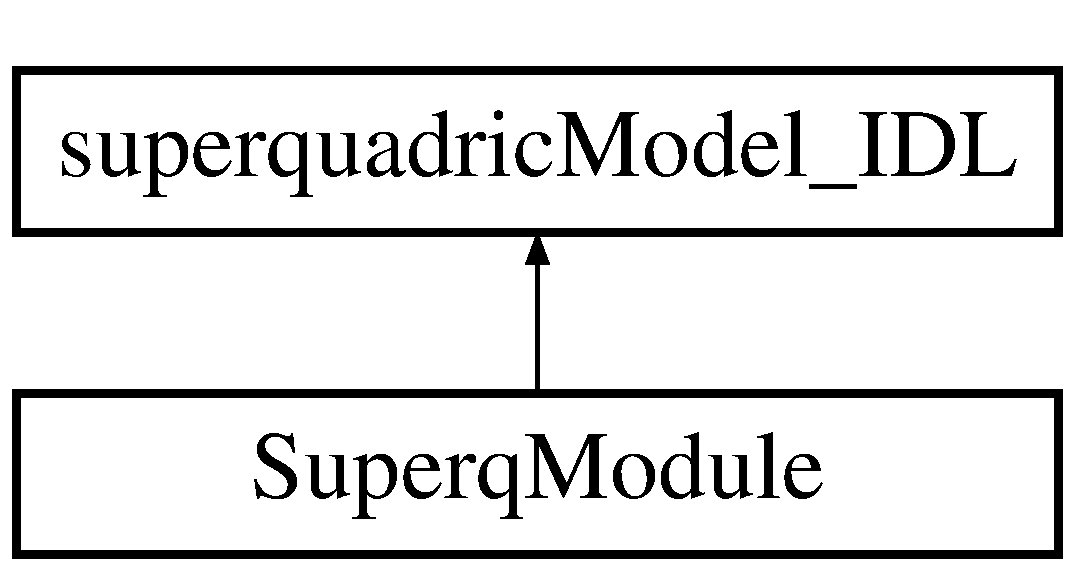
\includegraphics[height=2.000000cm]{classSuperqModule}
\end{center}
\end{figure}
\subsection*{Public Member Functions}
\begin{DoxyCompactItemize}
\item 
double \mbox{\hyperlink{classSuperqModule_aeec20285d89c1542d1b91c05c0f82539}{get\+Period}} ()
\begin{DoxyCompactList}\small\item\em Get period function of RF module. \end{DoxyCompactList}\item 
\mbox{\label{classSuperqModule_adba43b8815167f66e940bd80ab944af3}} 
bool \mbox{\hyperlink{classSuperqModule_adba43b8815167f66e940bd80ab944af3}{update\+Module}} ()
\begin{DoxyCompactList}\small\item\em update\+Module function of RF module \end{DoxyCompactList}\item 
\mbox{\label{classSuperqModule_a99527edc64196d4a9136416331fd5dd1}} 
bool \mbox{\hyperlink{classSuperqModule_a99527edc64196d4a9136416331fd5dd1}{configure}} (yarp\+::os\+::\+Resource\+Finder \&rf)
\begin{DoxyCompactList}\small\item\em configure function of RF module \end{DoxyCompactList}\item 
\mbox{\label{classSuperqModule_aca14ea8a02d8dbdef9a023da4c336891}} 
bool \mbox{\hyperlink{classSuperqModule_aca14ea8a02d8dbdef9a023da4c336891}{interrupt\+Module}} ()
\begin{DoxyCompactList}\small\item\em interrupt module function of RF module \end{DoxyCompactList}\item 
\mbox{\label{classSuperqModule_a6f88e21fe14a124919ffb07e26c04d15}} 
bool \mbox{\hyperlink{classSuperqModule_a6f88e21fe14a124919ffb07e26c04d15}{close}} ()
\begin{DoxyCompactList}\small\item\em close function of RF module \end{DoxyCompactList}\item 
\mbox{\label{classSuperqModule_a045733615dbe0c97f714dde4ea47a164}} 
bool \mbox{\hyperlink{classSuperqModule_a045733615dbe0c97f714dde4ea47a164}{config\+On\+Off}} (yarp\+::os\+::\+Resource\+Finder \&rf)
\begin{DoxyCompactList}\small\item\em Configure all on/off options. \end{DoxyCompactList}\item 
\mbox{\label{classSuperqModule_abe9bafeec746eb23da8f89cada86849e}} 
bool \mbox{\hyperlink{classSuperqModule_abe9bafeec746eb23da8f89cada86849e}{config\+Filter}} (yarp\+::os\+::\+Resource\+Finder \&rf)
\begin{DoxyCompactList}\small\item\em Configure point cloud filter options. \end{DoxyCompactList}\item 
\mbox{\label{classSuperqModule_a706feb064c09186585a97422603e6278}} 
bool \mbox{\hyperlink{classSuperqModule_a706feb064c09186585a97422603e6278}{config\+Filter\+Superq}} (yarp\+::os\+::\+Resource\+Finder \&rf)
\begin{DoxyCompactList}\small\item\em Configure superquadric filter options. \end{DoxyCompactList}\item 
\mbox{\label{classSuperqModule_aa27116ca1ef35ae86459aad82f4c53cb}} 
bool \mbox{\hyperlink{classSuperqModule_aa27116ca1ef35ae86459aad82f4c53cb}{config\+Services}} (yarp\+::os\+::\+Resource\+Finder \&rf)
\begin{DoxyCompactList}\small\item\em Open ports for communication. \end{DoxyCompactList}\item 
\mbox{\label{classSuperqModule_a36f445a18edc230bcd119b098143204f}} 
bool \mbox{\hyperlink{classSuperqModule_a36f445a18edc230bcd119b098143204f}{config\+Superq}} (yarp\+::os\+::\+Resource\+Finder \&rf)
\begin{DoxyCompactList}\small\item\em Configure superquadric computation otpions. \end{DoxyCompactList}\item 
\mbox{\label{classSuperqModule_ac92cfd73d4a1e08013051681ccb2e687}} 
bool \mbox{\hyperlink{classSuperqModule_ac92cfd73d4a1e08013051681ccb2e687}{config\+Viewer}} (yarp\+::os\+::\+Resource\+Finder \&rf)
\begin{DoxyCompactList}\small\item\em Configure visualization options. \end{DoxyCompactList}\item 
\mbox{\label{classSuperqModule_ada9aa974cf680e4f6e5507c2dc463856}} 
void \mbox{\hyperlink{classSuperqModule_ada9aa974cf680e4f6e5507c2dc463856}{save\+Superq}} ()
\begin{DoxyCompactList}\small\item\em Save computed superquadric. \end{DoxyCompactList}\item 
bool \mbox{\hyperlink{classSuperqModule_a90826fc53859ecf126f22a2569611b2c}{set\+\_\+save\+\_\+points}} (const std\+::string \&entry)
\begin{DoxyCompactList}\small\item\em Set if to save or not the used point cloud. \end{DoxyCompactList}\item 
std\+::string \mbox{\hyperlink{classSuperqModule_adfeeea091edd0d32d388b072f4fc9d93}{get\+\_\+save\+\_\+points}} ()
\begin{DoxyCompactList}\small\item\em Get if the used point cloud is saved or not. \end{DoxyCompactList}\item 
\mbox{\label{classSuperqModule_a0e6af855b1a0f647ff4b9deca973c55d}} 
bool \mbox{\hyperlink{classSuperqModule_a0e6af855b1a0f647ff4b9deca973c55d}{read\+Point\+Cloud}} ()
\begin{DoxyCompactList}\small\item\em In offline mode, read the point cloud from a txt file. \end{DoxyCompactList}\item 
virtual yarp\+::os\+::\+Property \mbox{\hyperlink{classsuperquadricModel__IDL_a10039bb93445066d9dd29d8f6c9ef6c5}{get\+\_\+superq}} (const std\+::vector$<$ yarp\+::sig\+::\+Vector $>$ \&point\+\_\+cloud, const bool filtered\+\_\+or\+\_\+not, const bool reset\+\_\+or\+\_\+not)
\begin{DoxyCompactList}\small\item\em Get the parameters of the reconstructed superquadric. \end{DoxyCompactList}\item 
\mbox{\label{classsuperquadricModel__IDL_ac72a24dddca13978d7adcd5cf4f40b1f}} 
virtual bool {\bfseries read} (yarp\+::os\+::\+Connection\+Reader \&connection)
\item 
\mbox{\label{classsuperquadricModel__IDL_a263ca3dc1c7a21cc3ac40caadc95cf3d}} 
virtual std\+::vector$<$ std\+::string $>$ {\bfseries help} (const std\+::string \&function\+Name=\char`\"{}-\/-\/all\char`\"{})
\end{DoxyCompactItemize}
\subsection*{Protected Member Functions}
\begin{DoxyCompactItemize}
\item 
\mbox{\label{classSuperqModule_a561e16c3b62e17a2fb96193c079bd970}} 
bool {\bfseries attach} (yarp\+::os\+::\+Rpc\+Server \&source)
\item 
bool \mbox{\hyperlink{classSuperqModule_ae9f0cfead2c367e4c3aa25292b5c42c6}{set\+\_\+tag\+\_\+file}} (const std\+::string \&\mbox{\hyperlink{classSuperqModule_a06b5f43aeaa26b5ca5961670f8883ab4}{tag\+\_\+file}})
\begin{DoxyCompactList}\small\item\em Set a tag name for saving the superquadric. \end{DoxyCompactList}\item 
std\+::string \mbox{\hyperlink{classSuperqModule_ac5475155a5a1b05e5fdef54699cef1a6}{get\+\_\+tag\+\_\+file}} ()
\begin{DoxyCompactList}\small\item\em Get the tag name used for saving the superquadric. \end{DoxyCompactList}\item 
std\+::string \mbox{\hyperlink{classSuperqModule_a89be4778051c4dd19339021448f89b41}{get\+\_\+visualization}} ()
\begin{DoxyCompactList}\small\item\em Return if visualization is on or off. \end{DoxyCompactList}\item 
bool \mbox{\hyperlink{classSuperqModule_ae4fc54ad89b3ee72ab5ea8c8b5065866}{set\+\_\+visualization}} (const std\+::string \&e)
\begin{DoxyCompactList}\small\item\em Set if visualization is on or off. \end{DoxyCompactList}\item 
yarp\+::os\+::\+Property \mbox{\hyperlink{classSuperqModule_a4a28afabfeac67e807dcc32845b41e0c}{get\+\_\+superq}} (const std\+::vector$<$ yarp\+::sig\+::\+Vector $>$ \&blob)
\begin{DoxyCompactList}\small\item\em Return the computed superquadric, given the 2D blob of the object. \end{DoxyCompactList}\item 
bool \mbox{\hyperlink{classSuperqModule_aa5a3fb751dd83d96004fceebab14c139}{send\+\_\+point\+\_\+clouds}} (const std\+::vector$<$ yarp\+::sig\+::\+Vector $>$ \&p)
\begin{DoxyCompactList}\small\item\em Get the point cloud for computing the superquadric. \end{DoxyCompactList}\item 
bool \mbox{\hyperlink{classSuperqModule_ae234e2b5b715e64ef928905964660122}{reset\+\_\+filter}} ()
\begin{DoxyCompactList}\small\item\em Reset median filter for improving superquadric estimation. \end{DoxyCompactList}\item 
yarp\+::os\+::\+Property \mbox{\hyperlink{classSuperqModule_aa6825617672381dcf3eb81dc643f0aaa}{get\+\_\+superq\+\_\+filtered}} ()
\begin{DoxyCompactList}\small\item\em Return the filtered superquadric. \end{DoxyCompactList}\item 
yarp\+::os\+::\+Property \mbox{\hyperlink{classSuperqModule_ae2935a960968a6354462a728e16d60b0}{fill\+Property}} (const yarp\+::sig\+::\+Vector \&sol)
\begin{DoxyCompactList}\small\item\em Property fill the property with the superquadric solution. \end{DoxyCompactList}\item 
bool \mbox{\hyperlink{classSuperqModule_a408203d0119443fb61544f84dafff8a4}{set\+\_\+points\+\_\+filtering}} (const std\+::string \&entry)
\begin{DoxyCompactList}\small\item\em Set if to filter or not the point cloud. \end{DoxyCompactList}\item 
std\+::string \mbox{\hyperlink{classSuperqModule_a60c8ff17436cc55a3e9b704dd6c2529b}{get\+\_\+points\+\_\+filtering}} ()
\begin{DoxyCompactList}\small\item\em Get if the point cloud is filtered or not. \end{DoxyCompactList}\item 
bool \mbox{\hyperlink{classSuperqModule_a902d4a48d1a919ff9d9b1f7d1c132577}{set\+\_\+superq\+\_\+filtering}} (const std\+::string \&entry)
\begin{DoxyCompactList}\small\item\em Set if to filter or not the superquadric. \end{DoxyCompactList}\item 
std\+::string \mbox{\hyperlink{classSuperqModule_a66cb1b371b92687d851b5ca23174198b}{get\+\_\+superq\+\_\+filtering}} ()
\begin{DoxyCompactList}\small\item\em Get if the superquadric is filtered or not. \end{DoxyCompactList}\item 
yarp\+::os\+::\+Property \mbox{\hyperlink{classSuperqModule_a18822e0a99dc0b13479f20960c577fb9}{get\+\_\+options}} (const std\+::string \&field)
\begin{DoxyCompactList}\small\item\em Get options of a given field\+: visualization, optimization, filtering. \end{DoxyCompactList}\item 
bool \mbox{\hyperlink{classSuperqModule_a32ccf59ac0572ca77883237dd2d12890}{set\+\_\+options}} (const yarp\+::os\+::\+Property \&new\+Options, const std\+::string \&field)
\begin{DoxyCompactList}\small\item\em Set options of specified field\+: visualization, optimization, filtering. \end{DoxyCompactList}\item 
bool \mbox{\hyperlink{classSuperqModule_aa00f3e123ab12a0c65f864f2900c36e4}{set\+\_\+object\+\_\+class}} (const std\+::string \&objclass)
\begin{DoxyCompactList}\small\item\em Set object class for improving superquadric estimation. \end{DoxyCompactList}\end{DoxyCompactItemize}
\subsection*{Protected Attributes}
\begin{DoxyCompactItemize}
\item 
\mbox{\label{classSuperqModule_ada2b94883ea2a69f9fab8cb045a5a138}} 
int \mbox{\hyperlink{classSuperqModule_ada2b94883ea2a69f9fab8cb045a5a138}{r}}
\begin{DoxyCompactList}\small\item\em Red value for visualization. \end{DoxyCompactList}\item 
\mbox{\label{classSuperqModule_a1d40ba1a934cd176b0365116597814da}} 
int \mbox{\hyperlink{classSuperqModule_a1d40ba1a934cd176b0365116597814da}{g}}
\begin{DoxyCompactList}\small\item\em Green value for visualization. \end{DoxyCompactList}\item 
\mbox{\label{classSuperqModule_a048daff404a4f8d8dd83072f5e7675cd}} 
int \mbox{\hyperlink{classSuperqModule_a048daff404a4f8d8dd83072f5e7675cd}{b}}
\begin{DoxyCompactList}\small\item\em Blue value for visualization. \end{DoxyCompactList}\item 
\mbox{\label{classSuperqModule_a4fbfa7613a6f89c61454b61acf288b9f}} 
int \mbox{\hyperlink{classSuperqModule_a4fbfa7613a6f89c61454b61acf288b9f}{count}}
\begin{DoxyCompactList}\small\item\em Count variable. \end{DoxyCompactList}\item 
\mbox{\label{classSuperqModule_aa778e1c9f9b6627b72bafe1c45e097b9}} 
int \mbox{\hyperlink{classSuperqModule_aa778e1c9f9b6627b72bafe1c45e097b9}{rate}}
\begin{DoxyCompactList}\small\item\em Computation thread rate. \end{DoxyCompactList}\item 
\mbox{\label{classSuperqModule_ad0dab1b5c69a32f877eac1ca745a0cbc}} 
int \mbox{\hyperlink{classSuperqModule_ad0dab1b5c69a32f877eac1ca745a0cbc}{rate\+\_\+vis}}
\begin{DoxyCompactList}\small\item\em Visualization thread rate. \end{DoxyCompactList}\item 
\mbox{\label{classSuperqModule_a06b5f43aeaa26b5ca5961670f8883ab4}} 
std\+::string \mbox{\hyperlink{classSuperqModule_a06b5f43aeaa26b5ca5961670f8883ab4}{tag\+\_\+file}}
\begin{DoxyCompactList}\small\item\em Tag name of files for saving 3D points. \end{DoxyCompactList}\item 
\mbox{\label{classSuperqModule_aa767064e88d01bc7cd8fb2038c63e150}} 
std\+::string \mbox{\hyperlink{classSuperqModule_aa767064e88d01bc7cd8fb2038c63e150}{home\+Context\+Path}}
\begin{DoxyCompactList}\small\item\em Path where code context is located. \end{DoxyCompactList}\item 
\mbox{\label{classSuperqModule_aa719adf35eb593b75e0f0930aa18a4f7}} 
yarp\+::os\+::\+Const\+String \mbox{\hyperlink{classSuperqModule_aa719adf35eb593b75e0f0930aa18a4f7}{point\+Cloud\+File\+Name}}
\begin{DoxyCompactList}\small\item\em Pointcloud name file in case the module runs offline. \end{DoxyCompactList}\item 
\mbox{\label{classSuperqModule_aac8cd7786df2bc4aeb0f7290807c4c49}} 
std\+::string \mbox{\hyperlink{classSuperqModule_aac8cd7786df2bc4aeb0f7290807c4c49}{output\+File\+Name}}
\begin{DoxyCompactList}\small\item\em Output file name saving the estimated superquadric. \end{DoxyCompactList}\item 
\mbox{\label{classSuperqModule_a2a3cbd0eb9042671dbbc457f5cb25c29}} 
std\+::vector$<$ cv\+::\+Point $>$ \mbox{\hyperlink{classSuperqModule_a2a3cbd0eb9042671dbbc457f5cb25c29}{contour}}
\begin{DoxyCompactList}\small\item\em Open\+CV variable for blob extraction. \end{DoxyCompactList}\item 
\mbox{\label{classSuperqModule_a9d894dfd7e6564ee41a98619c8178584}} 
std\+::deque$<$ yarp\+::sig\+::\+Vector $>$ \mbox{\hyperlink{classSuperqModule_a9d894dfd7e6564ee41a98619c8178584}{points}}
\begin{DoxyCompactList}\small\item\em 3D points used for reconstructing the superquadric \end{DoxyCompactList}\item 
\mbox{\label{classSuperqModule_a94cb68f67f8c51a188e12db5fad27565}} 
std\+::deque$<$ yarp\+::sig\+::\+Vector $>$ \mbox{\hyperlink{classSuperqModule_a94cb68f67f8c51a188e12db5fad27565}{points\+\_\+aux}}
\begin{DoxyCompactList}\small\item\em 3D points auxiliary used for reconstructing the superquadric \end{DoxyCompactList}\item 
\mbox{\label{classSuperqModule_a571d62b869e77e87b5fad6a13a72f813}} 
std\+::deque$<$ cv\+::\+Point $>$ \mbox{\hyperlink{classSuperqModule_a571d62b869e77e87b5fad6a13a72f813}{blob\+\_\+points}}
\begin{DoxyCompactList}\small\item\em 2D points of the segmented object \end{DoxyCompactList}\item 
\mbox{\label{classSuperqModule_a0751c095220723cf7d8b25b5d45a92e1}} 
double \mbox{\hyperlink{classSuperqModule_a0751c095220723cf7d8b25b5d45a92e1}{radius}}
\begin{DoxyCompactList}\small\item\em Radius for spatial density filter. \end{DoxyCompactList}\item 
\mbox{\label{classSuperqModule_ab7798766f824ed28f1f4dae8a3f1356c}} 
int \mbox{\hyperlink{classSuperqModule_ab7798766f824ed28f1f4dae8a3f1356c}{nn\+Threshold}}
\begin{DoxyCompactList}\small\item\em Density threshold for spatial density filter. \end{DoxyCompactList}\item 
\mbox{\label{classSuperqModule_a9cc4835f5280e71876b76331288b8dc2}} 
int {\bfseries num\+Vertices}
\item 
\mbox{\label{classSuperqModule_ae2d1a7a9301e43d148afda36fddd87b4}} 
int \mbox{\hyperlink{classSuperqModule_ae2d1a7a9301e43d148afda36fddd87b4}{median\+\_\+order}}
\begin{DoxyCompactList}\small\item\em Median filder order. \end{DoxyCompactList}\item 
\mbox{\label{classSuperqModule_a96b534ae428e744f2b44d35866490fdc}} 
int \mbox{\hyperlink{classSuperqModule_a96b534ae428e744f2b44d35866490fdc}{min\+\_\+median\+\_\+order}}
\begin{DoxyCompactList}\small\item\em Minimum median filder order allowed. \end{DoxyCompactList}\item 
\mbox{\label{classSuperqModule_a1d1b6f621d446969d9a8aa9abfafa7f9}} 
int \mbox{\hyperlink{classSuperqModule_a1d1b6f621d446969d9a8aa9abfafa7f9}{max\+\_\+median\+\_\+order}}
\begin{DoxyCompactList}\small\item\em Maximum median filder order allowed. \end{DoxyCompactList}\item 
\mbox{\label{classSuperqModule_a1409f49f4c5824ec604ce214654d3e22}} 
int \mbox{\hyperlink{classSuperqModule_a1409f49f4c5824ec604ce214654d3e22}{new\+\_\+median\+\_\+order}}
\begin{DoxyCompactList}\small\item\em New median filder order estimated. \end{DoxyCompactList}\item 
\mbox{\label{classSuperqModule_aa1bc1b1b7d3ef1b287d0c8d15d9a51bc}} 
bool \mbox{\hyperlink{classSuperqModule_aa1bc1b1b7d3ef1b287d0c8d15d9a51bc}{filter\+\_\+points}}
\begin{DoxyCompactList}\small\item\em Boolean variable for enabling point cloud filtering. \end{DoxyCompactList}\item 
\mbox{\label{classSuperqModule_a07ff8af914d2f3b5ae9fbc03b94954e7}} 
bool \mbox{\hyperlink{classSuperqModule_a07ff8af914d2f3b5ae9fbc03b94954e7}{fixed\+\_\+window}}
\begin{DoxyCompactList}\small\item\em Boolean variable for enabling the use of a fixed window during the median filter. \end{DoxyCompactList}\item 
\mbox{\label{classSuperqModule_a3e824c0b36749d3e9d2ff755004b7472}} 
bool \mbox{\hyperlink{classSuperqModule_a3e824c0b36749d3e9d2ff755004b7472}{filter\+\_\+superq}}
\begin{DoxyCompactList}\small\item\em Boolean variable for enabling superquadric filtering. \end{DoxyCompactList}\item 
\mbox{\label{classSuperqModule_a1f1963d5a8947368cec96d4fbcc3ec79}} 
std\+::string \mbox{\hyperlink{classSuperqModule_a1f1963d5a8947368cec96d4fbcc3ec79}{what\+\_\+to\+\_\+plot}}
\begin{DoxyCompactList}\small\item\em String used for deciding what to plot\+: \char`\"{}points\char`\"{} or \char`\"{}superq\char`\"{}. \end{DoxyCompactList}\item 
\mbox{\label{classSuperqModule_a226a730b20160c8e6483bd3b1064a7bc}} 
double \mbox{\hyperlink{classSuperqModule_a226a730b20160c8e6483bd3b1064a7bc}{threshold\+\_\+median}}
\begin{DoxyCompactList}\small\item\em Threshold for velocity estimation for median order. \end{DoxyCompactList}\item 
\mbox{\label{classSuperqModule_ace8ceaaf035427634c78f3d720ab2432}} 
double \mbox{\hyperlink{classSuperqModule_ace8ceaaf035427634c78f3d720ab2432}{min\+\_\+norm\+\_\+vel}}
\begin{DoxyCompactList}\small\item\em Minimum norm of velocity for considering the object moving. \end{DoxyCompactList}\item 
\mbox{\label{classSuperqModule_adfab63f5b7aad436d9833898ea23602a}} 
bool \mbox{\hyperlink{classSuperqModule_adfab63f5b7aad436d9833898ea23602a}{mode\+\_\+online}}
\begin{DoxyCompactList}\small\item\em Boolean variable for enabling online or offline mode. \end{DoxyCompactList}\item 
\mbox{\label{classSuperqModule_aecdc7d85514cc472b7a91982d6b1f58d}} 
bool \mbox{\hyperlink{classSuperqModule_aecdc7d85514cc472b7a91982d6b1f58d}{visualization\+\_\+on}}
\begin{DoxyCompactList}\small\item\em Boolean variable for enabling visualization. \end{DoxyCompactList}\item 
\mbox{\label{classSuperqModule_a46bddbc5530c3086005ad07281bc5ae9}} 
bool \mbox{\hyperlink{classSuperqModule_a46bddbc5530c3086005ad07281bc5ae9}{go\+\_\+on}}
\begin{DoxyCompactList}\small\item\em Boolean variable for going to the next step of the state machine. \end{DoxyCompactList}\item 
\mbox{\label{classSuperqModule_ad3f77b480fd86b554fabf882c090ddc1}} 
bool \mbox{\hyperlink{classSuperqModule_ad3f77b480fd86b554fabf882c090ddc1}{reset}}
\begin{DoxyCompactList}\small\item\em Boolean variable for resetting the median filter. \end{DoxyCompactList}\item 
\mbox{\label{classSuperqModule_a67a8bc8f0d0464efc29caf5465f256e6}} 
bool \mbox{\hyperlink{classSuperqModule_a67a8bc8f0d0464efc29caf5465f256e6}{save\+\_\+points}}
\begin{DoxyCompactList}\small\item\em Boolean variable for enabling point cloud saving. \end{DoxyCompactList}\item 
\mbox{\label{classSuperqModule_ad4843804d3d340b725debf434e5347b5}} 
double \mbox{\hyperlink{classSuperqModule_ad4843804d3d340b725debf434e5347b5}{tol}}
\begin{DoxyCompactList}\small\item\em Tolerance of the optimization problem. \end{DoxyCompactList}\item 
\mbox{\label{classSuperqModule_a01f96b54badeaf38908355577586a4c0}} 
double {\bfseries sum}
\item 
\mbox{\label{classSuperqModule_aace6a0e5aa42c5e376a5e60397a4dcea}} 
double \mbox{\hyperlink{classSuperqModule_aace6a0e5aa42c5e376a5e60397a4dcea}{max\+\_\+cpu\+\_\+time}}
\begin{DoxyCompactList}\small\item\em Max cpu time allowed for solving the optimization problem. \end{DoxyCompactList}\item 
\mbox{\label{classSuperqModule_ab3c64f8ffe227d91ab3fcc8983589b3a}} 
int \mbox{\hyperlink{classSuperqModule_ab3c64f8ffe227d91ab3fcc8983589b3a}{acceptable\+\_\+iter}}
\begin{DoxyCompactList}\small\item\em Acceptable iter of Ipopt algorithm. \end{DoxyCompactList}\item 
\mbox{\label{classSuperqModule_ae130c3d3d0ac884336761ded94731f1b}} 
int \mbox{\hyperlink{classSuperqModule_ae130c3d3d0ac884336761ded94731f1b}{max\+\_\+iter}}
\begin{DoxyCompactList}\small\item\em Maximum iteration allowed of Ipopt algorithm. \end{DoxyCompactList}\item 
\mbox{\label{classSuperqModule_ae796a494cc0be47bf8888e9f876784dc}} 
int \mbox{\hyperlink{classSuperqModule_ae796a494cc0be47bf8888e9f876784dc}{optimizer\+\_\+points}}
\begin{DoxyCompactList}\small\item\em Number of 3D points used for optimization. \end{DoxyCompactList}\item 
\mbox{\label{classSuperqModule_a29a3eb467fb15cb219b43c70a8cfda8a}} 
std\+::string \mbox{\hyperlink{classSuperqModule_a29a3eb467fb15cb219b43c70a8cfda8a}{mu\+\_\+strategy}}
\begin{DoxyCompactList}\small\item\em Mu strategy of the Ipopt algorithm. \end{DoxyCompactList}\item 
\mbox{\label{classSuperqModule_a01f9c7e0ec759b78c782483aaf2f0085}} 
std\+::string \mbox{\hyperlink{classSuperqModule_a01f9c7e0ec759b78c782483aaf2f0085}{nlp\+\_\+scaling\+\_\+method}}
\begin{DoxyCompactList}\small\item\em N\+LP scaling method of the Ipopt algorithm. \end{DoxyCompactList}\item 
\mbox{\label{classSuperqModule_a8b845bdc0c6d35d90141968502ca9d96}} 
yarp\+::sig\+::\+Vector \mbox{\hyperlink{classSuperqModule_a8b845bdc0c6d35d90141968502ca9d96}{x}}
\begin{DoxyCompactList}\small\item\em Estimated superquadric. \end{DoxyCompactList}\item 
\mbox{\label{classSuperqModule_adb96b7bb58edc83b70dcd4781b51130a}} 
yarp\+::sig\+::\+Vector \mbox{\hyperlink{classSuperqModule_adb96b7bb58edc83b70dcd4781b51130a}{x\+\_\+filtered}}
\begin{DoxyCompactList}\small\item\em Filtered superquadric. \end{DoxyCompactList}\item 
\mbox{\label{classSuperqModule_a981bafe724d09df7beb3c10fa96a8980}} 
double \mbox{\hyperlink{classSuperqModule_a981bafe724d09df7beb3c10fa96a8980}{t\+\_\+superq}}
\begin{DoxyCompactList}\small\item\em Time required for computing superquadric. \end{DoxyCompactList}\item 
\mbox{\label{classSuperqModule_a28517e736a16c5e7dfde3bcbec6bf5fd}} 
std\+::deque$<$ double $>$ \mbox{\hyperlink{classSuperqModule_a28517e736a16c5e7dfde3bcbec6bf5fd}{times\+\_\+superq}}
\begin{DoxyCompactList}\small\item\em Times used for computing several superquadrics. \end{DoxyCompactList}\item 
\mbox{\label{classSuperqModule_ac4b02568e69c9ed84739bb252a31def6}} 
double \mbox{\hyperlink{classSuperqModule_ac4b02568e69c9ed84739bb252a31def6}{t\+\_\+vis}}
\begin{DoxyCompactList}\small\item\em Time for visualization. \end{DoxyCompactList}\item 
\mbox{\label{classSuperqModule_af8194f823d1dfc5072988680d71aab08}} 
std\+::deque$<$ double $>$ \mbox{\hyperlink{classSuperqModule_af8194f823d1dfc5072988680d71aab08}{times\+\_\+vis}}
\begin{DoxyCompactList}\small\item\em Collections of times required for visualization. \end{DoxyCompactList}\item 
\mbox{\label{classSuperqModule_ac73ad3c50ea4fe58e35a722c37a7f99e}} 
yarp\+::os\+::\+Buffered\+Port$<$ yarp\+::os\+::\+Property $>$ \mbox{\hyperlink{classSuperqModule_ac73ad3c50ea4fe58e35a722c37a7f99e}{port\+Superq}}
\begin{DoxyCompactList}\small\item\em Port for streaming the computed superquadric. \end{DoxyCompactList}\item 
\mbox{\label{classSuperqModule_ab44a4843a8cb533d80d55df985b11448}} 
yarp\+::os\+::\+Rpc\+Server \mbox{\hyperlink{classSuperqModule_ab44a4843a8cb533d80d55df985b11448}{port\+Rpc}}
\begin{DoxyCompactList}\small\item\em Rpc port for interaction. \end{DoxyCompactList}\item 
\mbox{\label{classSuperqModule_ae8e5d7e83ef5cd80a44ce6a3bcc74cd7}} 
int \mbox{\hyperlink{classSuperqModule_ae8e5d7e83ef5cd80a44ce6a3bcc74cd7}{vis\+\_\+points}}
\begin{DoxyCompactList}\small\item\em Number of points used for visualization. \end{DoxyCompactList}\item 
\mbox{\label{classSuperqModule_a73aa4f6c8c4c9142fb5456c9cdaaf6b6}} 
int \mbox{\hyperlink{classSuperqModule_a73aa4f6c8c4c9142fb5456c9cdaaf6b6}{vis\+\_\+step}}
\begin{DoxyCompactList}\small\item\em Number of visualization step. \end{DoxyCompactList}\item 
\mbox{\label{classSuperqModule_a016da49606647c049c4b857a32c633c6}} 
std\+::string \mbox{\hyperlink{classSuperqModule_a016da49606647c049c4b857a32c633c6}{eye}}
\begin{DoxyCompactList}\small\item\em Eye camera selected. \end{DoxyCompactList}\item 
\mbox{\label{classSuperqModule_ab0570fcea5cbee6364f780cca614164d}} 
yarp\+::sig\+::\+Matrix {\bfseries R}
\item 
\mbox{\label{classSuperqModule_acf23ebc65162db020fd4e25ca73ea165}} 
yarp\+::sig\+::\+Matrix {\bfseries H}
\item 
\mbox{\label{classSuperqModule_ac6ee7467d82e835c0d1b2e35236e4aaf}} 
yarp\+::sig\+::\+Matrix {\bfseries K}
\item 
\mbox{\label{classSuperqModule_a80128e303c0d59016e41493ca50cc94e}} 
yarp\+::sig\+::\+Vector {\bfseries point}
\item 
\mbox{\label{classSuperqModule_ab8daf379295df5a47ced6f06acfe0df9}} 
yarp\+::sig\+::\+Vector {\bfseries point1}
\item 
\mbox{\label{classSuperqModule_a8839fda8369d4e2e73714cc1db6e0f5e}} 
yarp\+::sig\+::\+Vector {\bfseries point2D}
\item 
\mbox{\label{classSuperqModule_a15f7523202cf192d71f188db2647e50c}} 
std\+::deque$<$ int $>$ \mbox{\hyperlink{classSuperqModule_a15f7523202cf192d71f188db2647e50c}{Color}}
\begin{DoxyCompactList}\small\item\em Color used for visualization. \end{DoxyCompactList}\item 
\mbox{\label{classSuperqModule_a1ce22879df6c4586ed72a3e3b67609bb}} 
yarp\+::dev\+::\+Poly\+Driver \mbox{\hyperlink{classSuperqModule_a1ce22879df6c4586ed72a3e3b67609bb}{Gaze\+Ctrl}}
\begin{DoxyCompactList}\small\item\em Gaze Control driver for visualization. \end{DoxyCompactList}\item 
\mbox{\label{classSuperqModule_a00ea631bed0909310e2e505f0aca688f}} 
yarp\+::dev\+::\+I\+Gaze\+Control $\ast$ \mbox{\hyperlink{classSuperqModule_a00ea631bed0909310e2e505f0aca688f}{igaze}}
\begin{DoxyCompactList}\small\item\em Gaze Control interface. \end{DoxyCompactList}\item 
\mbox{\label{classSuperqModule_ac781b86f89aab354c250c17cff49c2d8}} 
yarp\+::os\+::\+Resource\+Finder $\ast$ {\bfseries rf}
\item 
\mbox{\label{classSuperqModule_a7246f334af9922695d716a5afb4ce89e}} 
double {\bfseries t}
\item 
\mbox{\label{classSuperqModule_aa0788b39ee666e4cd09ea4c59421dc24}} 
double {\bfseries t0}
\item 
\mbox{\label{classSuperqModule_aa45e8a64fbe20bc54d9f303369a618aa}} 
std\+::deque$<$ std\+::string $>$ {\bfseries advanced\+\_\+params}
\item 
\mbox{\label{classSuperqModule_a04543bfe968184ff3ee55905c90f12ac}} 
yarp\+::os\+::\+Mutex {\bfseries mutex}
\item 
\mbox{\label{classSuperqModule_aa6671c2457e2044f3823d671a9b7e6ea}} 
yarp\+::os\+::\+Mutex {\bfseries mutex\+\_\+shared}
\item 
\mbox{\label{classSuperqModule_ae26497c030a1ecd16b98096c5842f383}} 
std\+::string {\bfseries object\+\_\+class}
\item 
\mbox{\label{classSuperqModule_adab3d841bcfd52387bb6dd861fddf424}} 
\mbox{\hyperlink{classSuperqComputation}{Superq\+Computation}} $\ast$ \mbox{\hyperlink{classSuperqModule_adab3d841bcfd52387bb6dd861fddf424}{superq\+Com}}
\begin{DoxyCompactList}\small\item\em \mbox{\hyperlink{classSuperqComputation}{Superq\+Computation}} class actually computes the superquadric. \end{DoxyCompactList}\item 
\mbox{\label{classSuperqModule_a91b35d4f88a0bfda1bb6f0bcfa6976b1}} 
\mbox{\hyperlink{classSuperqVisualization}{Superq\+Visualization}} $\ast$ \mbox{\hyperlink{classSuperqModule_a91b35d4f88a0bfda1bb6f0bcfa6976b1}{superq\+Vis}}
\begin{DoxyCompactList}\small\item\em \mbox{\hyperlink{classSuperqVisualization}{Superq\+Visualization}} class shows the estimated superquadric. \end{DoxyCompactList}\item 
\mbox{\label{classSuperqModule_a86c20777e5607bb326216605bab0e222}} 
yarp\+::os\+::\+Property \mbox{\hyperlink{classSuperqModule_a86c20777e5607bb326216605bab0e222}{filter\+\_\+points\+\_\+par}}
\begin{DoxyCompactList}\small\item\em Parameters of point cloud filter. \end{DoxyCompactList}\item 
\mbox{\label{classSuperqModule_ac9c130b5960c724aed615bbf6ac17b50}} 
yarp\+::os\+::\+Property \mbox{\hyperlink{classSuperqModule_ac9c130b5960c724aed615bbf6ac17b50}{filter\+\_\+superq\+\_\+par}}
\begin{DoxyCompactList}\small\item\em Parameters of superquadric filter. \end{DoxyCompactList}\item 
\mbox{\label{classSuperqModule_a6469063a5f34843741f727696d1803e1}} 
yarp\+::os\+::\+Property \mbox{\hyperlink{classSuperqModule_a6469063a5f34843741f727696d1803e1}{ipopt\+\_\+par}}
\begin{DoxyCompactList}\small\item\em Parameters of the Ipopt optimization problem. \end{DoxyCompactList}\end{DoxyCompactItemize}


\subsection{Detailed Description}
The \mbox{\hyperlink{classSuperqModule}{Superq\+Module}} class handle the superquadric computation and visualization, the point cloud and superquadric filtering and the interaction with the user. 

It is used to set all the parameters (offline and online) and to launch all the thread for superquadric computation and visualization. 

Definition at line 40 of file superq\+Module.\+h.



\subsection{Member Function Documentation}
\mbox{\label{classSuperqModule_ae2935a960968a6354462a728e16d60b0}} 
\index{Superq\+Module@{Superq\+Module}!fill\+Property@{fill\+Property}}
\index{fill\+Property@{fill\+Property}!Superq\+Module@{Superq\+Module}}
\subsubsection{\texorpdfstring{fill\+Property()}{fillProperty()}}
{\footnotesize\ttfamily Property Superq\+Module\+::fill\+Property (\begin{DoxyParamCaption}\item[{const yarp\+::sig\+::\+Vector \&}]{sol }\end{DoxyParamCaption})\hspace{0.3cm}{\ttfamily [protected]}}



Property fill the property with the superquadric solution. 


\begin{DoxyParams}{Parameters}
{\em sol} & is a Vector of the computed superquadric \\
\hline
\end{DoxyParams}
\begin{DoxyReturn}{Returns}
a Property with the solution 
\end{DoxyReturn}


Definition at line 187 of file superq\+Module.\+cpp.


\begin{DoxyCode}
188 \{
189     Property superq;
190 
191     Bottle bottle;
192     Bottle &b1=bottle.addList();
193     b1.addDouble(sol[0]); b1.addDouble(sol[1]); b1.addDouble(sol[2]);
194     superq.put(\textcolor{stringliteral}{"dimensions"}, bottle.get(0));
195 
196     Bottle &b2=bottle.addList();
197     b2.addDouble(sol[3]); b2.addDouble(sol[4]);
198     superq.put(\textcolor{stringliteral}{"exponents"}, bottle.get(1));
199 
200     Bottle &b3=bottle.addList();
201     b3.addDouble(sol[5]); b3.addDouble(sol[6]); b3.addDouble(sol[7]);
202     superq.put(\textcolor{stringliteral}{"center"}, bottle.get(2));
203 
204     Bottle &b4=bottle.addList();
205     Vector orient=dcm2axis(euler2dcm(sol.subVector(8,10)));
206     b4.addDouble(orient[0]); b4.addDouble(orient[1]); b4.addDouble(orient[2]); b4.addDouble(orient[3]);
207     superq.put(\textcolor{stringliteral}{"orientation"}, bottle.get(3));
208     \textcolor{keywordflow}{return} superq;
209 \}
\end{DoxyCode}
\mbox{\label{classSuperqModule_a18822e0a99dc0b13479f20960c577fb9}} 
\index{Superq\+Module@{Superq\+Module}!get\+\_\+options@{get\+\_\+options}}
\index{get\+\_\+options@{get\+\_\+options}!Superq\+Module@{Superq\+Module}}
\subsubsection{\texorpdfstring{get\+\_\+options()}{get\_options()}}
{\footnotesize\ttfamily Property Superq\+Module\+::get\+\_\+options (\begin{DoxyParamCaption}\item[{const std\+::string \&}]{field }\end{DoxyParamCaption})\hspace{0.3cm}{\ttfamily [protected]}, {\ttfamily [virtual]}}



Get options of a given field\+: visualization, optimization, filtering. 


\begin{DoxyParams}{Parameters}
{\em field} & is one of the field of options \\
\hline
\end{DoxyParams}
\begin{DoxyReturn}{Returns}
property with the options of interested 
\end{DoxyReturn}


Reimplemented from \mbox{\hyperlink{classsuperquadricModel__IDL_a50b388a29852f9d8b57a0bbb276d4675}{superquadric\+Model\+\_\+\+I\+DL}}.



Definition at line 330 of file superq\+Module.\+cpp.


\begin{DoxyCode}
331 \{
332     Property advOptions;
333     \textcolor{keywordflow}{if} (field==\textcolor{stringliteral}{"points\_filter"})
334         advOptions=superqCom->getPointsFilterPar();
335     \textcolor{keywordflow}{else} \textcolor{keywordflow}{if} (field==\textcolor{stringliteral}{"superq\_filter"})
336         advOptions=superqCom->getSuperqFilterPar();
337     \textcolor{keywordflow}{else} \textcolor{keywordflow}{if} (field==\textcolor{stringliteral}{"optimization"})
338         advOptions=superqCom->getIpoptPar();
339     \textcolor{keywordflow}{else} \textcolor{keywordflow}{if} (field==\textcolor{stringliteral}{"visualization"})
340         advOptions=superqVis->getPar();
341     \textcolor{keywordflow}{else} \textcolor{keywordflow}{if} (field==\textcolor{stringliteral}{"statistics"})
342     \{
343         advOptions.put(\textcolor{stringliteral}{"average\_computation\_time"}, t_superq);
344         advOptions.put(\textcolor{stringliteral}{"average\_visualization\_time"}, t_vis);
345     \}       
346 
347     \textcolor{keywordflow}{return} advOptions;
348 \}
\end{DoxyCode}
\mbox{\label{classSuperqModule_a60c8ff17436cc55a3e9b704dd6c2529b}} 
\index{Superq\+Module@{Superq\+Module}!get\+\_\+points\+\_\+filtering@{get\+\_\+points\+\_\+filtering}}
\index{get\+\_\+points\+\_\+filtering@{get\+\_\+points\+\_\+filtering}!Superq\+Module@{Superq\+Module}}
\subsubsection{\texorpdfstring{get\+\_\+points\+\_\+filtering()}{get\_points\_filtering()}}
{\footnotesize\ttfamily string Superq\+Module\+::get\+\_\+points\+\_\+filtering (\begin{DoxyParamCaption}{ }\end{DoxyParamCaption})\hspace{0.3cm}{\ttfamily [protected]}, {\ttfamily [virtual]}}



Get if the point cloud is filtered or not. 

\begin{DoxyReturn}{Returns}
\char`\"{}on\char`\"{} or \char`\"{}off\char`\"{} 
\end{DoxyReturn}


Reimplemented from \mbox{\hyperlink{classsuperquadricModel__IDL_aa490ebcf39414aaaae41d5095267abb9}{superquadric\+Model\+\_\+\+I\+DL}}.



Definition at line 242 of file superq\+Module.\+cpp.


\begin{DoxyCode}
243 \{
244     \textcolor{keywordflow}{if} (filter_points)
245     \{
246         \textcolor{keywordflow}{return} \textcolor{stringliteral}{"on"};
247     \}
248     \textcolor{keywordflow}{else}
249     \{
250         \textcolor{keywordflow}{return} \textcolor{stringliteral}{"off"};
251     \}
252 \}
\end{DoxyCode}
\mbox{\label{classSuperqModule_adfeeea091edd0d32d388b072f4fc9d93}} 
\index{Superq\+Module@{Superq\+Module}!get\+\_\+save\+\_\+points@{get\+\_\+save\+\_\+points}}
\index{get\+\_\+save\+\_\+points@{get\+\_\+save\+\_\+points}!Superq\+Module@{Superq\+Module}}
\subsubsection{\texorpdfstring{get\+\_\+save\+\_\+points()}{get\_save\_points()}}
{\footnotesize\ttfamily string Superq\+Module\+::get\+\_\+save\+\_\+points (\begin{DoxyParamCaption}{ }\end{DoxyParamCaption})\hspace{0.3cm}{\ttfamily [virtual]}}



Get if the used point cloud is saved or not. 

\begin{DoxyReturn}{Returns}
\char`\"{}on\char`\"{} or \char`\"{}off\char`\"{} 
\end{DoxyReturn}


Reimplemented from \mbox{\hyperlink{classsuperquadricModel__IDL_a4b101fe118a1ee912468562bde0b0df4}{superquadric\+Model\+\_\+\+I\+DL}}.



Definition at line 304 of file superq\+Module.\+cpp.


\begin{DoxyCode}
305 \{
306     \textcolor{keywordflow}{if} (save_points)
307     \{
308         \textcolor{keywordflow}{return} \textcolor{stringliteral}{"on"};
309     \}
310     \textcolor{keywordflow}{else}
311     \{
312         \textcolor{keywordflow}{return} \textcolor{stringliteral}{"off"};
313     \}
314 \}
\end{DoxyCode}
\mbox{\label{classsuperquadricModel__IDL_a10039bb93445066d9dd29d8f6c9ef6c5}} 
\index{Superq\+Module@{Superq\+Module}!get\+\_\+superq@{get\+\_\+superq}}
\index{get\+\_\+superq@{get\+\_\+superq}!Superq\+Module@{Superq\+Module}}
\subsubsection{\texorpdfstring{get\+\_\+superq()}{get\_superq()}\hspace{0.1cm}{\footnotesize\ttfamily [1/2]}}
{\footnotesize\ttfamily virtual yarp\+::os\+::\+Property superquadric\+Model\+\_\+\+I\+D\+L\+::get\+\_\+superq (\begin{DoxyParamCaption}\item[{const std\+::vector$<$ yarp\+::sig\+::\+Vector $>$ \&}]{point\+\_\+cloud,  }\item[{const bool}]{filtered\+\_\+or\+\_\+not,  }\item[{const bool}]{reset\+\_\+or\+\_\+not }\end{DoxyParamCaption})\hspace{0.3cm}{\ttfamily [virtual]}, {\ttfamily [inherited]}}



Get the parameters of the reconstructed superquadric. 


\begin{DoxyParams}{Parameters}
{\em point\+\_\+cloud} & is the 3D point cloud of the object we want to model with the superquadric, for instance\+: ((100.\+0 102.\+0) (100.\+0 103.\+0) ... ). \\
\hline
{\em filtered\+\_\+or\+\_\+not} & is a bool variable specifing if we want the superquadric to be filtered (true/1) or not (false/0). \\
\hline
{\em reset\+\_\+or\+\_\+not} & is a bool variable specifing if we want to reset the superquadric filtered (if enabled) or not. \\
\hline
\end{DoxyParams}
\begin{DoxyReturn}{Returns}
the 12 parameters (x0, .. x11) of the current superquadric. In particular, the parameters are grouped in a Property as follows\+: \char`\"{}dimensions\char`\"{} (x0, x1, x2) are the three semi-\/axes lenghts; \char`\"{}exponents\char`\"{} (x3 and x4) are the exponents, responsible for the superquadric shape; \char`\"{}center\char`\"{}(x5, x6, x7) contains the coordinate of the superquadric center; and \char`\"{}orientation\char`\"{} (x8, x9, 10, x11) is the axis-\/angle representation obtained from the Euler angles. 
\end{DoxyReturn}
\mbox{\label{classSuperqModule_a4a28afabfeac67e807dcc32845b41e0c}} 
\index{Superq\+Module@{Superq\+Module}!get\+\_\+superq@{get\+\_\+superq}}
\index{get\+\_\+superq@{get\+\_\+superq}!Superq\+Module@{Superq\+Module}}
\subsubsection{\texorpdfstring{get\+\_\+superq()}{get\_superq()}\hspace{0.1cm}{\footnotesize\ttfamily [2/2]}}
{\footnotesize\ttfamily Property Superq\+Module\+::get\+\_\+superq (\begin{DoxyParamCaption}\item[{const std\+::vector$<$ yarp\+::sig\+::\+Vector $>$ \&}]{blob }\end{DoxyParamCaption})\hspace{0.3cm}{\ttfamily [protected]}}



Return the computed superquadric, given the 2D blob of the object. 


\begin{DoxyParams}{Parameters}
{\em blob} & is the 2D blob of the object \\
\hline
\end{DoxyParams}
\begin{DoxyReturn}{Returns}
a property with the estimated superquadric 
\end{DoxyReturn}


Definition at line 99 of file superq\+Module.\+cpp.


\begin{DoxyCode}
100 \{
101     Property superq;
102 
103     LockGuard lg(mutex);
104 
105     superqCom->setPar(\textcolor{stringliteral}{"object\_class"}, object\_class);
106 
107     superqCom->setPar(\textcolor{stringliteral}{"one\_shot"}, \textcolor{stringliteral}{"on"});
108 
109     deque<Vector> p\_aux;
110     
111     \textcolor{keywordflow}{for} (\textcolor{keywordtype}{size\_t} i=0; i<p.size(); i++)
112         p\_aux.push\_back(p[i]);
113 
114     superqCom->sendPoints(p\_aux);
115 
116     superqCom->run();
117 
118     Vector sol(11,0.0);
119     sol=superqCom->getSolution(0);
120 
121     superqCom->setPar(\textcolor{stringliteral}{"one\_shot"}, \textcolor{stringliteral}{"off"});
122 
123     p\_aux.clear();
124     superqCom->sendPoints(p\_aux);
125 
126     superq=fillProperty(sol);
127 
128     \textcolor{keywordflow}{return} superq;
129 \}
\end{DoxyCode}
\mbox{\label{classSuperqModule_aa6825617672381dcf3eb81dc643f0aaa}} 
\index{Superq\+Module@{Superq\+Module}!get\+\_\+superq\+\_\+filtered@{get\+\_\+superq\+\_\+filtered}}
\index{get\+\_\+superq\+\_\+filtered@{get\+\_\+superq\+\_\+filtered}!Superq\+Module@{Superq\+Module}}
\subsubsection{\texorpdfstring{get\+\_\+superq\+\_\+filtered()}{get\_superq\_filtered()}}
{\footnotesize\ttfamily Property Superq\+Module\+::get\+\_\+superq\+\_\+filtered (\begin{DoxyParamCaption}{ }\end{DoxyParamCaption})\hspace{0.3cm}{\ttfamily [protected]}}



Return the filtered superquadric. 

\begin{DoxyReturn}{Returns}
a property with the filtered superquadric 
\end{DoxyReturn}


Definition at line 170 of file superq\+Module.\+cpp.


\begin{DoxyCode}
171 \{
172     Property superq;
173     Vector sol(11,0.0);
174     sol=superqCom->getSolution(1);
175 
176     superqCom->setPar(\textcolor{stringliteral}{"one\_shot"}, \textcolor{stringliteral}{"off"});
177     deque<Vector> p\_aux;
178     p\_aux.clear();
179     superqCom->sendPoints(p\_aux);
180 
181     superq=fillProperty(sol);
182 
183     \textcolor{keywordflow}{return} superq;
184 \}
\end{DoxyCode}
\mbox{\label{classSuperqModule_a66cb1b371b92687d851b5ca23174198b}} 
\index{Superq\+Module@{Superq\+Module}!get\+\_\+superq\+\_\+filtering@{get\+\_\+superq\+\_\+filtering}}
\index{get\+\_\+superq\+\_\+filtering@{get\+\_\+superq\+\_\+filtering}!Superq\+Module@{Superq\+Module}}
\subsubsection{\texorpdfstring{get\+\_\+superq\+\_\+filtering()}{get\_superq\_filtering()}}
{\footnotesize\ttfamily string Superq\+Module\+::get\+\_\+superq\+\_\+filtering (\begin{DoxyParamCaption}{ }\end{DoxyParamCaption})\hspace{0.3cm}{\ttfamily [protected]}, {\ttfamily [virtual]}}



Get if the superquadric is filtered or not. 

\begin{DoxyReturn}{Returns}
\char`\"{}on\char`\"{} or \char`\"{}off\char`\"{} 
\end{DoxyReturn}


Reimplemented from \mbox{\hyperlink{classsuperquadricModel__IDL_af99d29d42b96b8db6c90c5fd48cfb253}{superquadric\+Model\+\_\+\+I\+DL}}.



Definition at line 291 of file superq\+Module.\+cpp.


\begin{DoxyCode}
292 \{
293     \textcolor{keywordflow}{if} (filter_superq)
294     \{
295         \textcolor{keywordflow}{return} \textcolor{stringliteral}{"on"};
296     \}
297     \textcolor{keywordflow}{else}
298     \{
299         \textcolor{keywordflow}{return} \textcolor{stringliteral}{"off"};
300     \}
301 \}
\end{DoxyCode}
\mbox{\label{classSuperqModule_ac5475155a5a1b05e5fdef54699cef1a6}} 
\index{Superq\+Module@{Superq\+Module}!get\+\_\+tag\+\_\+file@{get\+\_\+tag\+\_\+file}}
\index{get\+\_\+tag\+\_\+file@{get\+\_\+tag\+\_\+file}!Superq\+Module@{Superq\+Module}}
\subsubsection{\texorpdfstring{get\+\_\+tag\+\_\+file()}{get\_tag\_file()}}
{\footnotesize\ttfamily string Superq\+Module\+::get\+\_\+tag\+\_\+file (\begin{DoxyParamCaption}{ }\end{DoxyParamCaption})\hspace{0.3cm}{\ttfamily [protected]}, {\ttfamily [virtual]}}



Get the tag name used for saving the superquadric. 

\begin{DoxyReturn}{Returns}
the currect name of the file used for saving 
\end{DoxyReturn}


Reimplemented from \mbox{\hyperlink{classsuperquadricModel__IDL_a6d39eaa247aec65fe2bfefbdace4ec85}{superquadric\+Model\+\_\+\+I\+DL}}.



Definition at line 57 of file superq\+Module.\+cpp.


\begin{DoxyCode}
58 \{
59     \textcolor{keywordflow}{return} tag_file;
60 \}
\end{DoxyCode}
\mbox{\label{classSuperqModule_a89be4778051c4dd19339021448f89b41}} 
\index{Superq\+Module@{Superq\+Module}!get\+\_\+visualization@{get\+\_\+visualization}}
\index{get\+\_\+visualization@{get\+\_\+visualization}!Superq\+Module@{Superq\+Module}}
\subsubsection{\texorpdfstring{get\+\_\+visualization()}{get\_visualization()}}
{\footnotesize\ttfamily string Superq\+Module\+::get\+\_\+visualization (\begin{DoxyParamCaption}{ }\end{DoxyParamCaption})\hspace{0.3cm}{\ttfamily [protected]}, {\ttfamily [virtual]}}



Return if visualization is on or off. 

\begin{DoxyReturn}{Returns}
\char`\"{}on\char`\"{} or \char`\"{}off\char`\"{} 
\end{DoxyReturn}


Reimplemented from \mbox{\hyperlink{classsuperquadricModel__IDL_a5d9f4f0622ba19b60218636dc108ef61}{superquadric\+Model\+\_\+\+I\+DL}}.



Definition at line 63 of file superq\+Module.\+cpp.


\begin{DoxyCode}
64 \{
65     \textcolor{keywordflow}{if} (visualization_on)
66         \textcolor{keywordflow}{return} \textcolor{stringliteral}{"on"};
67     \textcolor{keywordflow}{else}
68         \textcolor{keywordflow}{return} \textcolor{stringliteral}{"off"};
69 \}
\end{DoxyCode}
\mbox{\label{classSuperqModule_aeec20285d89c1542d1b91c05c0f82539}} 
\index{Superq\+Module@{Superq\+Module}!get\+Period@{get\+Period}}
\index{get\+Period@{get\+Period}!Superq\+Module@{Superq\+Module}}
\subsubsection{\texorpdfstring{get\+Period()}{getPeriod()}}
{\footnotesize\ttfamily double Superq\+Module\+::get\+Period (\begin{DoxyParamCaption}{ }\end{DoxyParamCaption})}



Get period function of RF module. 

\begin{DoxyReturn}{Returns}
the period 
\end{DoxyReturn}


Definition at line 376 of file superq\+Module.\+cpp.


\begin{DoxyCode}
377 \{
378     \textcolor{keywordflow}{return} 0.0;
379 \}
\end{DoxyCode}
\mbox{\label{classSuperqModule_ae234e2b5b715e64ef928905964660122}} 
\index{Superq\+Module@{Superq\+Module}!reset\+\_\+filter@{reset\+\_\+filter}}
\index{reset\+\_\+filter@{reset\+\_\+filter}!Superq\+Module@{Superq\+Module}}
\subsubsection{\texorpdfstring{reset\+\_\+filter()}{reset\_filter()}}
{\footnotesize\ttfamily bool Superq\+Module\+::reset\+\_\+filter (\begin{DoxyParamCaption}{ }\end{DoxyParamCaption})\hspace{0.3cm}{\ttfamily [protected]}}



Reset median filter for improving superquadric estimation. 

\begin{DoxyReturn}{Returns}
true 
\end{DoxyReturn}


Definition at line 162 of file superq\+Module.\+cpp.


\begin{DoxyCode}
163 \{
164     superqCom->resetMedianFilter();
165 
166     \textcolor{keywordflow}{return} \textcolor{keyword}{true};
167 \}
\end{DoxyCode}
\mbox{\label{classSuperqModule_aa5a3fb751dd83d96004fceebab14c139}} 
\index{Superq\+Module@{Superq\+Module}!send\+\_\+point\+\_\+clouds@{send\+\_\+point\+\_\+clouds}}
\index{send\+\_\+point\+\_\+clouds@{send\+\_\+point\+\_\+clouds}!Superq\+Module@{Superq\+Module}}
\subsubsection{\texorpdfstring{send\+\_\+point\+\_\+clouds()}{send\_point\_clouds()}}
{\footnotesize\ttfamily bool Superq\+Module\+::send\+\_\+point\+\_\+clouds (\begin{DoxyParamCaption}\item[{const std\+::vector$<$ yarp\+::sig\+::\+Vector $>$ \&}]{p }\end{DoxyParamCaption})\hspace{0.3cm}{\ttfamily [protected]}}



Get the point cloud for computing the superquadric. 


\begin{DoxyParams}{Parameters}
{\em p} & is the point cloud to be acquired \\
\hline
\end{DoxyParams}
\begin{DoxyReturn}{Returns}
true 
\end{DoxyReturn}


Definition at line 132 of file superq\+Module.\+cpp.


\begin{DoxyCode}
133 \{
134     \textcolor{keywordtype}{double} t, t\_fin;  
135     
136     t=Time::now();
137 
138     superqCom->setPar(\textcolor{stringliteral}{"object\_class"}, object\_class);
139 
140     yDebug()<<\textcolor{stringliteral}{"Time operations  after set par 1"}<<Time::now() - t;
141 
142     superqCom->setPar(\textcolor{stringliteral}{"one\_shot"}, \textcolor{stringliteral}{"on"});
143 
144     yDebug()<<\textcolor{stringliteral}{"Time operations after set par 2"}<<Time::now() - t;
145 
146     deque<Vector> p\_aux;
147 
148     \textcolor{keywordflow}{for} (\textcolor{keywordtype}{size\_t} i=0; i<p.size(); i++)
149         p\_aux.push\_back(p[i]);
150 
151     superqCom->sendPoints(p\_aux);
152     yDebug()<<\textcolor{stringliteral}{"Time operations send points "}<<Time::now() - t;
153 
154     t\_fin= Time::now() - t;
155 
156     yDebug()<<\textcolor{stringliteral}{"Time operations  final"}<<t\_fin;
157 
158     \textcolor{keywordflow}{return} \textcolor{keyword}{true};
159 \}
\end{DoxyCode}
\mbox{\label{classSuperqModule_aa00f3e123ab12a0c65f864f2900c36e4}} 
\index{Superq\+Module@{Superq\+Module}!set\+\_\+object\+\_\+class@{set\+\_\+object\+\_\+class}}
\index{set\+\_\+object\+\_\+class@{set\+\_\+object\+\_\+class}!Superq\+Module@{Superq\+Module}}
\subsubsection{\texorpdfstring{set\+\_\+object\+\_\+class()}{set\_object\_class()}}
{\footnotesize\ttfamily bool Superq\+Module\+::set\+\_\+object\+\_\+class (\begin{DoxyParamCaption}\item[{const std\+::string \&}]{objclass }\end{DoxyParamCaption})\hspace{0.3cm}{\ttfamily [protected]}}



Set object class for improving superquadric estimation. 


\begin{DoxyParams}{Parameters}
{\em objclass} & is the object class (according to the shape) \\
\hline
\end{DoxyParams}
\begin{DoxyReturn}{Returns}
true/false on success/failure 
\end{DoxyReturn}


Definition at line 368 of file superq\+Module.\+cpp.


\begin{DoxyCode}
369 \{
370     object\_class=objclass;
371 
372     \textcolor{keywordflow}{return} \textcolor{keyword}{true};
373 \}
\end{DoxyCode}
\mbox{\label{classSuperqModule_a32ccf59ac0572ca77883237dd2d12890}} 
\index{Superq\+Module@{Superq\+Module}!set\+\_\+options@{set\+\_\+options}}
\index{set\+\_\+options@{set\+\_\+options}!Superq\+Module@{Superq\+Module}}
\subsubsection{\texorpdfstring{set\+\_\+options()}{set\_options()}}
{\footnotesize\ttfamily bool Superq\+Module\+::set\+\_\+options (\begin{DoxyParamCaption}\item[{const yarp\+::os\+::\+Property \&}]{new\+Options,  }\item[{const std\+::string \&}]{field }\end{DoxyParamCaption})\hspace{0.3cm}{\ttfamily [protected]}, {\ttfamily [virtual]}}



Set options of specified field\+: visualization, optimization, filtering. 


\begin{DoxyParams}{Parameters}
{\em new\+Options} & is a property with the options to be set \\
\hline
{\em field} & is the field of the options to be set \\
\hline
\end{DoxyParams}
\begin{DoxyReturn}{Returns}
true/false on success/failure 
\end{DoxyReturn}


Reimplemented from \mbox{\hyperlink{classsuperquadricModel__IDL_a575e0b591f07206b0d6c29e5cfeead37}{superquadric\+Model\+\_\+\+I\+DL}}.



Definition at line 351 of file superq\+Module.\+cpp.


\begin{DoxyCode}
352 \{
353     \textcolor{keywordflow}{if} (field==\textcolor{stringliteral}{"points\_filter"})
354         superqCom->setPointsFilterPar(newOptions, \textcolor{keyword}{false});
355     \textcolor{keywordflow}{else} \textcolor{keywordflow}{if} (field==\textcolor{stringliteral}{"superq\_filter"})
356         superqCom->setSuperqFilterPar(newOptions, \textcolor{keyword}{false});
357     \textcolor{keywordflow}{else} \textcolor{keywordflow}{if} (field==\textcolor{stringliteral}{"optimization"})
358         superqCom->setIpoptPar(newOptions, \textcolor{keyword}{false});
359     \textcolor{keywordflow}{else} \textcolor{keywordflow}{if} (field==\textcolor{stringliteral}{"visualization"})
360         superqVis->setPar(newOptions, \textcolor{keyword}{false});
361     \textcolor{keywordflow}{else}
362         \textcolor{keywordflow}{return} \textcolor{keyword}{false};
363 
364     \textcolor{keywordflow}{return} \textcolor{keyword}{true};
365 \}
\end{DoxyCode}
\mbox{\label{classSuperqModule_a408203d0119443fb61544f84dafff8a4}} 
\index{Superq\+Module@{Superq\+Module}!set\+\_\+points\+\_\+filtering@{set\+\_\+points\+\_\+filtering}}
\index{set\+\_\+points\+\_\+filtering@{set\+\_\+points\+\_\+filtering}!Superq\+Module@{Superq\+Module}}
\subsubsection{\texorpdfstring{set\+\_\+points\+\_\+filtering()}{set\_points\_filtering()}}
{\footnotesize\ttfamily bool Superq\+Module\+::set\+\_\+points\+\_\+filtering (\begin{DoxyParamCaption}\item[{const std\+::string \&}]{entry }\end{DoxyParamCaption})\hspace{0.3cm}{\ttfamily [protected]}, {\ttfamily [virtual]}}



Set if to filter or not the point cloud. 


\begin{DoxyParams}{Parameters}
{\em entre} & can be \char`\"{}on\char`\"{} or \char`\"{}off\char`\"{} \\
\hline
\end{DoxyParams}
\begin{DoxyReturn}{Returns}
true/false on success/failure 
\end{DoxyReturn}


Reimplemented from \mbox{\hyperlink{classsuperquadricModel__IDL_a1a2080d797a81b46b0dffa86b5367e15}{superquadric\+Model\+\_\+\+I\+DL}}.



Definition at line 212 of file superq\+Module.\+cpp.


\begin{DoxyCode}
213 \{
214     \textcolor{keywordflow}{if} ((entry==\textcolor{stringliteral}{"on"}) || (entry==\textcolor{stringliteral}{"off"}))
215     \{
216         LockGuard lg(mutex);
217         filter_points=(entry==\textcolor{stringliteral}{"on"});
218         \textcolor{keywordflow}{if} (filter_points)
219         \{
220             Property options;
221             options.put(\textcolor{stringliteral}{"filter\_radius"}, radius);
222             options.put(\textcolor{stringliteral}{"filter\_nnThreshold"}, nnThreshold);
223             superqCom->setPointsFilterPar(options, \textcolor{keyword}{false});
224             superqCom->setPar(\textcolor{stringliteral}{"filter\_points"}, \textcolor{stringliteral}{"on"});
225         \}
226         \textcolor{keywordflow}{else}
227             superqCom->setPar(\textcolor{stringliteral}{"filter\_points"}, \textcolor{stringliteral}{"off"});
228 
229         yInfo()<<\textcolor{stringliteral}{"[SuperqModule]: filter\_points "}<<filter_points;
230         yInfo()<<\textcolor{stringliteral}{"[SuperqModule]: radius        "}<<radius;
231         yInfo()<<\textcolor{stringliteral}{"[SuperqModule]: nn-thrshold   "}<<nnThreshold;
232 
233         \textcolor{keywordflow}{return} \textcolor{keyword}{true};    
234     \}
235     \textcolor{keywordflow}{else}
236     \{        
237         \textcolor{keywordflow}{return} \textcolor{keyword}{false};
238     \}
239 \}
\end{DoxyCode}
\mbox{\label{classSuperqModule_a90826fc53859ecf126f22a2569611b2c}} 
\index{Superq\+Module@{Superq\+Module}!set\+\_\+save\+\_\+points@{set\+\_\+save\+\_\+points}}
\index{set\+\_\+save\+\_\+points@{set\+\_\+save\+\_\+points}!Superq\+Module@{Superq\+Module}}
\subsubsection{\texorpdfstring{set\+\_\+save\+\_\+points()}{set\_save\_points()}}
{\footnotesize\ttfamily bool Superq\+Module\+::set\+\_\+save\+\_\+points (\begin{DoxyParamCaption}\item[{const std\+::string \&}]{entry }\end{DoxyParamCaption})\hspace{0.3cm}{\ttfamily [virtual]}}



Set if to save or not the used point cloud. 


\begin{DoxyParams}{Parameters}
{\em entry} & can be \char`\"{}on\char`\"{} or \char`\"{}off\char`\"{} \\
\hline
\end{DoxyParams}


Reimplemented from \mbox{\hyperlink{classsuperquadricModel__IDL_a8368b783845a3e5ae7e0706ee5b888c0}{superquadric\+Model\+\_\+\+I\+DL}}.



Definition at line 317 of file superq\+Module.\+cpp.


\begin{DoxyCode}
318 \{
319     \textcolor{keywordflow}{if} ((entry==\textcolor{stringliteral}{"on"}) || (entry==\textcolor{stringliteral}{"off"}))
320     \{
321         save_points=(entry==\textcolor{stringliteral}{"on"});
322         \textcolor{keywordflow}{if} (save_points)
323             superqCom->setPar(\textcolor{stringliteral}{"save\_points"}, \textcolor{stringliteral}{"on"});
324         \textcolor{keywordflow}{else}
325             superqCom->setPar(\textcolor{stringliteral}{"save\_points"}, \textcolor{stringliteral}{"off"});
326     \}    
327 \}
\end{DoxyCode}
\mbox{\label{classSuperqModule_a902d4a48d1a919ff9d9b1f7d1c132577}} 
\index{Superq\+Module@{Superq\+Module}!set\+\_\+superq\+\_\+filtering@{set\+\_\+superq\+\_\+filtering}}
\index{set\+\_\+superq\+\_\+filtering@{set\+\_\+superq\+\_\+filtering}!Superq\+Module@{Superq\+Module}}
\subsubsection{\texorpdfstring{set\+\_\+superq\+\_\+filtering()}{set\_superq\_filtering()}}
{\footnotesize\ttfamily bool Superq\+Module\+::set\+\_\+superq\+\_\+filtering (\begin{DoxyParamCaption}\item[{const std\+::string \&}]{entry }\end{DoxyParamCaption})\hspace{0.3cm}{\ttfamily [protected]}, {\ttfamily [virtual]}}



Set if to filter or not the superquadric. 


\begin{DoxyParams}{Parameters}
{\em entry} & can be \char`\"{}on\char`\"{} or \char`\"{}off\char`\"{} \\
\hline
\end{DoxyParams}
\begin{DoxyReturn}{Returns}
true/false on success/failure 
\end{DoxyReturn}


Reimplemented from \mbox{\hyperlink{classsuperquadricModel__IDL_af418edf09afd9374c5272d018c58e8a7}{superquadric\+Model\+\_\+\+I\+DL}}.



Definition at line 255 of file superq\+Module.\+cpp.


\begin{DoxyCode}
256 \{
257     \textcolor{keywordflow}{if} ((entry==\textcolor{stringliteral}{"on"}) || (entry==\textcolor{stringliteral}{"off"}))
258     \{
259         LockGuard lg(mutex);
260         filter_superq= (entry==\textcolor{stringliteral}{"on"});
261         \textcolor{keywordflow}{if} (filter_superq)
262         \{
263             Property options;
264             options.put(\textcolor{stringliteral}{"median\_order"}, median_order);
265             \textcolor{keywordflow}{if} (fixed_window)
266                 options.put(\textcolor{stringliteral}{"fixed\_window"}, \textcolor{stringliteral}{"on"});
267             \textcolor{keywordflow}{else}
268                 options.put(\textcolor{stringliteral}{"fixed\_window"}, \textcolor{stringliteral}{"off"});
269 
270             superqCom->setSuperqFilterPar(options, \textcolor{keyword}{false});
271             superqCom->setPar(\textcolor{stringliteral}{"filter\_superq"}, \textcolor{stringliteral}{"on"});
272         \}
273         \textcolor{keywordflow}{else}
274             superqCom->setPar(\textcolor{stringliteral}{"filter\_superq"}, \textcolor{stringliteral}{"off"});
275 
276         yInfo()<<\textcolor{stringliteral}{"[SuperqModule]: filter\_superq         "}<<filter_superq;
277         yInfo()<<\textcolor{stringliteral}{"[SuperqModule]: fixed\_window          "}<<fixed_window;
278         yInfo()<<\textcolor{stringliteral}{"[SuperqModule]: median\_order          "}<<median_order;
279         yInfo()<<\textcolor{stringliteral}{"[SuperqModule]: min\_median\_order      "}<<min_median_order;
280         yInfo()<<\textcolor{stringliteral}{"[SuperqModule]: max\_median\_order      "}<<max_median_order;
281 
282         \textcolor{keywordflow}{return} \textcolor{keyword}{true};        
283     \}
284     \textcolor{keywordflow}{else}
285     \{
286         \textcolor{keywordflow}{return} \textcolor{keyword}{false};
287     \}
288 \}
\end{DoxyCode}
\mbox{\label{classSuperqModule_ae9f0cfead2c367e4c3aa25292b5c42c6}} 
\index{Superq\+Module@{Superq\+Module}!set\+\_\+tag\+\_\+file@{set\+\_\+tag\+\_\+file}}
\index{set\+\_\+tag\+\_\+file@{set\+\_\+tag\+\_\+file}!Superq\+Module@{Superq\+Module}}
\subsubsection{\texorpdfstring{set\+\_\+tag\+\_\+file()}{set\_tag\_file()}}
{\footnotesize\ttfamily bool Superq\+Module\+::set\+\_\+tag\+\_\+file (\begin{DoxyParamCaption}\item[{const std\+::string \&}]{tag\+\_\+file }\end{DoxyParamCaption})\hspace{0.3cm}{\ttfamily [protected]}, {\ttfamily [virtual]}}



Set a tag name for saving the superquadric. 


\begin{DoxyParams}{Parameters}
{\em tag\+\_\+file} & is the name of the file where to save the superquadric \\
\hline
\end{DoxyParams}
\begin{DoxyReturn}{Returns}
true 
\end{DoxyReturn}


Reimplemented from \mbox{\hyperlink{classsuperquadricModel__IDL_a781426bfc4862e87ef75a4bbbfa33275}{superquadric\+Model\+\_\+\+I\+DL}}.



Definition at line 43 of file superq\+Module.\+cpp.


\begin{DoxyCode}
44 \{
45     LockGuard lg(mutex);
46 
47     tag_file=tag;
48     outputFileName=homeContextPath+\textcolor{stringliteral}{"/"}+tag_file+\textcolor{stringliteral}{".txt"};
49     yDebug()<<\textcolor{stringliteral}{" [SuperqModule]: File output "}<<outputFileName;
50 
51     superqCom->setPar(\textcolor{stringliteral}{"tag\_file"}, tag_file);
52 
53     \textcolor{keywordflow}{return} \textcolor{keyword}{true};
54 \}
\end{DoxyCode}
\mbox{\label{classSuperqModule_ae4fc54ad89b3ee72ab5ea8c8b5065866}} 
\index{Superq\+Module@{Superq\+Module}!set\+\_\+visualization@{set\+\_\+visualization}}
\index{set\+\_\+visualization@{set\+\_\+visualization}!Superq\+Module@{Superq\+Module}}
\subsubsection{\texorpdfstring{set\+\_\+visualization()}{set\_visualization()}}
{\footnotesize\ttfamily bool Superq\+Module\+::set\+\_\+visualization (\begin{DoxyParamCaption}\item[{const std\+::string \&}]{e }\end{DoxyParamCaption})\hspace{0.3cm}{\ttfamily [protected]}, {\ttfamily [virtual]}}



Set if visualization is on or off. 


\begin{DoxyParams}{Parameters}
{\em e} & can be \char`\"{}on\char`\"{} or \char`\"{}off\char`\"{} \\
\hline
\end{DoxyParams}
\begin{DoxyReturn}{Returns}
true/false on success/failure 
\end{DoxyReturn}


Reimplemented from \mbox{\hyperlink{classsuperquadricModel__IDL_a651c741e9b01b25d46be96b06b91011d}{superquadric\+Model\+\_\+\+I\+DL}}.



Definition at line 72 of file superq\+Module.\+cpp.


\begin{DoxyCode}
73 \{
74     \textcolor{keywordflow}{if} ((e==\textcolor{stringliteral}{"on"}) || (e==\textcolor{stringliteral}{"off"}))
75     \{
76         LockGuard lg(mutex);
77 
78         \textcolor{keywordflow}{if} ((visualization_on==\textcolor{keyword}{false}) && (e==\textcolor{stringliteral}{"on"}))
79         \{
80             superqVis->resume();
81 
82             visualization_on=\textcolor{keyword}{true};
83 
84         \}
85         \textcolor{keywordflow}{else} \textcolor{keywordflow}{if} ((visualization_on==\textcolor{keyword}{true}) && (e==\textcolor{stringliteral}{"off"}))
86         \{
87             superqVis->suspend();
88             visualization_on=\textcolor{keyword}{false};
89         \}
90         \textcolor{keywordflow}{return} \textcolor{keyword}{true};
91     \}
92     \textcolor{keywordflow}{else}
93     \{
94         \textcolor{keywordflow}{return} \textcolor{keyword}{false};
95     \}
96 \}
\end{DoxyCode}


The documentation for this class was generated from the following files\+:\begin{DoxyCompactItemize}
\item 
C\+:/\+Users/upattacini/\+Desktop/superquadric-\/model/include/superq\+Module.\+h\item 
C\+:/\+Users/upattacini/\+Desktop/superquadric-\/model/src/superq\+Module.\+cpp\end{DoxyCompactItemize}

\section{Super\+Quadric\+\_\+\+N\+LP Class Reference}
\label{classSuperQuadric__NLP}\index{Super\+Quadric\+\_\+\+N\+LP@{Super\+Quadric\+\_\+\+N\+LP}}


This class solves the optimization problem with the Ipopt software package and returns the estiamted superquadric, better fitting a given point cloud.  




{\ttfamily \#include $<$superquadric.\+h$>$}



Inherits T\+N\+LP.

\subsection*{Public Member Functions}
\begin{DoxyCompactItemize}
\item 
\mbox{\label{classSuperQuadric__NLP_a7e39371548648a9b8d9673084ed5407d}} 
void \mbox{\hyperlink{classSuperQuadric__NLP_a7e39371548648a9b8d9673084ed5407d}{init}} ()
\begin{DoxyCompactList}\small\item\em Init function. \end{DoxyCompactList}\item 
void \mbox{\hyperlink{classSuperQuadric__NLP_a6895a29435328142fcb31a4827742fa6}{set\+Points}} (const std\+::deque$<$ yarp\+::sig\+::\+Vector $>$ \&point\+\_\+cloud, const int \&optimizer\+\_\+points)
\begin{DoxyCompactList}\small\item\em Set point to be used for superquadric estimation. \end{DoxyCompactList}\item 
void \mbox{\hyperlink{classSuperQuadric__NLP_aebc2844bb4fb3ff0399fc8fef8198229}{configure}} (yarp\+::os\+::\+Resource\+Finder $\ast$rf, bool bounds\+\_\+aut, const std\+::string \&object\+\_\+class)
\begin{DoxyCompactList}\small\item\em Configure function. \end{DoxyCompactList}\item 
yarp\+::sig\+::\+Vector \mbox{\hyperlink{classSuperQuadric__NLP_a5f32c9a6ef0483ddade880a15db7d417}{get\+\_\+result}} () const
\begin{DoxyCompactList}\small\item\em Extract the solution. \end{DoxyCompactList}\item 
bool \mbox{\hyperlink{classSuperQuadric__NLP_a964efe0e0fe66464238f99885c6323bf}{read\+Matrix}} (const std\+::string \&tag, yarp\+::sig\+::\+Matrix \&matrix, const int \&dimension, yarp\+::os\+::\+Resource\+Finder $\ast$rf)
\begin{DoxyCompactList}\small\item\em Function for reading matrices from config files. \end{DoxyCompactList}\end{DoxyCompactItemize}
\subsection*{Data Fields}
\begin{DoxyCompactItemize}
\item 
\mbox{\label{classSuperQuadric__NLP_abf380018deaca365a8b7cd837f36f1fa}} 
yarp\+::sig\+::\+Vector \mbox{\hyperlink{classSuperQuadric__NLP_abf380018deaca365a8b7cd837f36f1fa}{solution}}
\begin{DoxyCompactList}\small\item\em Final solution. \end{DoxyCompactList}\item 
\mbox{\label{classSuperQuadric__NLP_a9577e3ef86a127dec53a64953926c288}} 
std\+::deque$<$ yarp\+::sig\+::\+Vector $>$ \mbox{\hyperlink{classSuperQuadric__NLP_a9577e3ef86a127dec53a64953926c288}{points\+\_\+downsampled}}
\begin{DoxyCompactList}\small\item\em 3D points actually used for superquadric estimation \end{DoxyCompactList}\end{DoxyCompactItemize}
\subsection*{Protected Member Functions}
\begin{DoxyCompactItemize}
\item 
bool \mbox{\hyperlink{classSuperQuadric__NLP_a2599f20c7a4c6eb3da7dec612098d1b4}{get\+\_\+nlp\+\_\+info}} (Ipopt\+::\+Index \&n, Ipopt\+::\+Index \&m, Ipopt\+::\+Index \&nnz\+\_\+jac\+\_\+g, Ipopt\+::\+Index \&nnz\+\_\+h\+\_\+lag, Ipopt\+::\+T\+N\+L\+P\+::\+Index\+Style\+Enum \&index\+\_\+style)
\begin{DoxyCompactList}\small\item\em Get info for the nonlinear problem to be solved with ipopt. \end{DoxyCompactList}\item 
\mbox{\label{classSuperQuadric__NLP_aaafe8516b6f3e68caf218f6cfb048c1b}} 
void \mbox{\hyperlink{classSuperQuadric__NLP_aaafe8516b6f3e68caf218f6cfb048c1b}{compute\+Bounds}} ()
\begin{DoxyCompactList}\small\item\em Compute bounds variable from the point cloud for speeding up optimization. \end{DoxyCompactList}\item 
bool \mbox{\hyperlink{classSuperQuadric__NLP_a9f303ff4d778230990fd151631c2d9d4}{get\+\_\+bounds\+\_\+info}} (Ipopt\+::\+Index n, Ipopt\+::\+Number $\ast$x\+\_\+l, Ipopt\+::\+Number $\ast$x\+\_\+u, Ipopt\+::\+Index m, Ipopt\+::\+Number $\ast$g\+\_\+l, Ipopt\+::\+Number $\ast$g\+\_\+u)
\begin{DoxyCompactList}\small\item\em Get variable bounds for the nonlinear problem to be solved with ipopt. \end{DoxyCompactList}\item 
bool \mbox{\hyperlink{classSuperQuadric__NLP_a05ec724269d1060c5e53112817938639}{get\+\_\+starting\+\_\+point}} (Ipopt\+::\+Index n, bool init\+\_\+x, Ipopt\+::\+Number $\ast$x, bool init\+\_\+z, Ipopt\+::\+Number $\ast$z\+\_\+L, Ipopt\+::\+Number $\ast$z\+\_\+U, Ipopt\+::\+Index m, bool init\+\_\+lambda, Ipopt\+::\+Number $\ast$lambda)
\begin{DoxyCompactList}\small\item\em Get the starting point for the nonlinear problem to be solved with ipopt. \end{DoxyCompactList}\item 
bool \mbox{\hyperlink{classSuperQuadric__NLP_ab33c41e6fa8674c1434aac9b18a62d37}{eval\+\_\+f}} (Ipopt\+::\+Index n, const Ipopt\+::\+Number $\ast$x, bool new\+\_\+x, Ipopt\+::\+Number \&obj\+\_\+value)
\begin{DoxyCompactList}\small\item\em Cost function of the nonlinear problem to be solved with ipopt. \end{DoxyCompactList}\item 
void \mbox{\hyperlink{classSuperQuadric__NLP_afaecc87e024a55c07d13f45b8e7af173}{F}} (const Ipopt\+::\+Number $\ast$x, std\+::deque$<$ yarp\+::sig\+::\+Vector $>$ \&points, bool \&new\+\_\+x)
\begin{DoxyCompactList}\small\item\em Auxiliary function for computing cost function of the nonlinear problem to be solved with ipopt. \end{DoxyCompactList}\item 
double \mbox{\hyperlink{classSuperQuadric__NLP_aa914a977bcaea04f375778085c40cb9a}{f}} (const Ipopt\+::\+Number $\ast$x, const yarp\+::sig\+::\+Matrix \&R, const yarp\+::sig\+::\+Vector \&point\+\_\+cloud)
\begin{DoxyCompactList}\small\item\em Auxiliary function for computing cost function of the nonlinear problem to be solved with ipopt. \end{DoxyCompactList}\item 
double \mbox{\hyperlink{classSuperQuadric__NLP_adc57687952c43086dff7b2da7c3456a8}{F\+\_\+v}} (const yarp\+::sig\+::\+Vector \&x, const std\+::deque$<$ yarp\+::sig\+::\+Vector $>$ \&points)
\begin{DoxyCompactList}\small\item\em Auxiliary function for computing the gradient of cost function of the nonlinear problem. \end{DoxyCompactList}\item 
double \mbox{\hyperlink{classSuperQuadric__NLP_a36f02b201ae96896b9627851199eb49c}{f\+\_\+v}} (const yarp\+::sig\+::\+Vector \&x, const yarp\+::sig\+::\+Matrix \&R, const yarp\+::sig\+::\+Vector \&point\+\_\+cloud)
\begin{DoxyCompactList}\small\item\em Auxiliary function for computing cost function of the nonlinear problem to be solved with ipopt. \end{DoxyCompactList}\item 
bool \mbox{\hyperlink{classSuperQuadric__NLP_a7ad18ed5adb66e686409183651de562c}{eval\+\_\+grad\+\_\+f}} (Ipopt\+::\+Index n, const Ipopt\+::\+Number $\ast$x, bool new\+\_\+x, Ipopt\+::\+Number $\ast$grad\+\_\+f)
\begin{DoxyCompactList}\small\item\em Gradient of the cost function of the nonlinear problem. \end{DoxyCompactList}\item 
bool \mbox{\hyperlink{classSuperQuadric__NLP_a43a2c0f905b6e38045bcb55a93ae8654}{eval\+\_\+g}} (Ipopt\+::\+Index n, const Ipopt\+::\+Number $\ast$x, bool new\+\_\+x, Ipopt\+::\+Index m, Ipopt\+::\+Number $\ast$g)
\begin{DoxyCompactList}\small\item\em Constraints of the nonlinear problem. \end{DoxyCompactList}\item 
bool \mbox{\hyperlink{classSuperQuadric__NLP_a2eac4aa901938d0637769c66d68aeec2}{eval\+\_\+jac\+\_\+g}} (Ipopt\+::\+Index n, const Ipopt\+::\+Number $\ast$x, bool new\+\_\+x, Ipopt\+::\+Index m, Ipopt\+::\+Index nele\+\_\+jac, Ipopt\+::\+Index $\ast$i\+Row, Ipopt\+::\+Index $\ast$j\+Col, Ipopt\+::\+Number $\ast$values)
\begin{DoxyCompactList}\small\item\em Jacobian of the constraints of the nonlinear problem. \end{DoxyCompactList}\item 
void \mbox{\hyperlink{classSuperQuadric__NLP_a7395729e42b83d083b88451620ede9c6}{compute\+X0}} (yarp\+::sig\+::\+Vector \&\mbox{\hyperlink{classSuperQuadric__NLP_a25e5121f404d68a8fa0122e803945f8b}{x0}}, std\+::deque$<$ yarp\+::sig\+::\+Vector $>$ \&point\+\_\+cloud)
\begin{DoxyCompactList}\small\item\em Compute a good starting point for the nonlinear problem. \end{DoxyCompactList}\item 
void \mbox{\hyperlink{classSuperQuadric__NLP_a6fd9bdffb81bfdfec56bae2efd58c270}{compute\+Initial\+Orientation}} (yarp\+::sig\+::\+Vector \&\mbox{\hyperlink{classSuperQuadric__NLP_a25e5121f404d68a8fa0122e803945f8b}{x0}}, std\+::deque$<$ yarp\+::sig\+::\+Vector $>$ \&point\+\_\+cloud)
\begin{DoxyCompactList}\small\item\em Compute initial superquadric orientation from the point cloud. \end{DoxyCompactList}\item 
yarp\+::sig\+::\+Matrix \mbox{\hyperlink{classSuperQuadric__NLP_a425745a725c4f0dba398a6b5389809a7}{compute\+Bounding\+Box}} (std\+::deque$<$ yarp\+::sig\+::\+Vector $>$ \&points, const yarp\+::sig\+::\+Vector \&\mbox{\hyperlink{classSuperQuadric__NLP_a25e5121f404d68a8fa0122e803945f8b}{x0}})
\begin{DoxyCompactList}\small\item\em Compute bounding box from the point cloud. \end{DoxyCompactList}\item 
void \mbox{\hyperlink{classSuperQuadric__NLP_a2f0b1fc45d42b0ee77c343ea7c227874}{finalize\+\_\+solution}} (Ipopt\+::\+Solver\+Return status, Ipopt\+::\+Index n, const Ipopt\+::\+Number $\ast$x, const Ipopt\+::\+Number $\ast$z\+\_\+L, const Ipopt\+::\+Number $\ast$z\+\_\+U, Ipopt\+::\+Index m, const Ipopt\+::\+Number $\ast$g, const Ipopt\+::\+Number $\ast$lambda, Ipopt\+::\+Number obj\+\_\+value, const Ipopt\+::\+Ipopt\+Data $\ast$ip\+\_\+data, Ipopt\+::\+Ipopt\+Calculated\+Quantities $\ast$ip\+\_\+cq)
\begin{DoxyCompactList}\small\item\em Finalize the solution. \end{DoxyCompactList}\end{DoxyCompactItemize}
\subsection*{Protected Attributes}
\begin{DoxyCompactItemize}
\item 
\mbox{\label{classSuperQuadric__NLP_ac4ae54a0a2bc47b2a984278a4e57400c}} 
bool \mbox{\hyperlink{classSuperQuadric__NLP_ac4ae54a0a2bc47b2a984278a4e57400c}{bounds\+\_\+automatic}}
\begin{DoxyCompactList}\small\item\em Boolean variable for enabling automatic bounds computation. \end{DoxyCompactList}\item 
\mbox{\label{classSuperQuadric__NLP_a4215586669b4e4e835993634290cac9a}} 
yarp\+::sig\+::\+Vector \mbox{\hyperlink{classSuperQuadric__NLP_a4215586669b4e4e835993634290cac9a}{x\+\_\+v}}
\begin{DoxyCompactList}\small\item\em Auxiliar vector for gradient computation. \end{DoxyCompactList}\item 
\mbox{\label{classSuperQuadric__NLP_a25e5121f404d68a8fa0122e803945f8b}} 
yarp\+::sig\+::\+Vector \mbox{\hyperlink{classSuperQuadric__NLP_a25e5121f404d68a8fa0122e803945f8b}{x0}}
\begin{DoxyCompactList}\small\item\em Starting point for the optimization problem. \end{DoxyCompactList}\item 
\mbox{\label{classSuperQuadric__NLP_a3300e78dabc6dc8fd7e959c176b8a32c}} 
yarp\+::sig\+::\+Matrix \mbox{\hyperlink{classSuperQuadric__NLP_a3300e78dabc6dc8fd7e959c176b8a32c}{bounds}}
\begin{DoxyCompactList}\small\item\em Bounds variable of the optimization problem. \end{DoxyCompactList}\item 
\mbox{\label{classSuperQuadric__NLP_ad0bf24004b855864ad0a498f9fb13c81}} 
double {\bfseries aux\+\_\+objvalue}
\item 
\mbox{\label{classSuperQuadric__NLP_a6806ddd4f4b035abbf7835e4b38931ca}} 
std\+::string \mbox{\hyperlink{classSuperQuadric__NLP_a6806ddd4f4b035abbf7835e4b38931ca}{obj\+\_\+class}}
\begin{DoxyCompactList}\small\item\em Object class\+: cylinder, sphere and box. \end{DoxyCompactList}\item 
\mbox{\label{classSuperQuadric__NLP_a7dc22430259697726ab6341fc2e95074}} 
yarp\+::os\+::\+Resource\+Finder $\ast$ {\bfseries rf}
\end{DoxyCompactItemize}


\subsection{Detailed Description}
This class solves the optimization problem with the Ipopt software package and returns the estiamted superquadric, better fitting a given point cloud. 

Definition at line 36 of file superquadric.\+h.



\subsection{Member Function Documentation}
\mbox{\label{classSuperQuadric__NLP_a425745a725c4f0dba398a6b5389809a7}} 
\index{Super\+Quadric\+\_\+\+N\+LP@{Super\+Quadric\+\_\+\+N\+LP}!compute\+Bounding\+Box@{compute\+Bounding\+Box}}
\index{compute\+Bounding\+Box@{compute\+Bounding\+Box}!Super\+Quadric\+\_\+\+N\+LP@{Super\+Quadric\+\_\+\+N\+LP}}
\subsubsection{\texorpdfstring{compute\+Bounding\+Box()}{computeBoundingBox()}}
{\footnotesize\ttfamily Matrix Super\+Quadric\+\_\+\+N\+L\+P\+::compute\+Bounding\+Box (\begin{DoxyParamCaption}\item[{std\+::deque$<$ yarp\+::sig\+::\+Vector $>$ \&}]{points,  }\item[{const yarp\+::sig\+::\+Vector \&}]{x0 }\end{DoxyParamCaption})\hspace{0.3cm}{\ttfamily [protected]}}



Compute bounding box from the point cloud. 


\begin{DoxyParams}{Parameters}
{\em points} & is the point cloud \\
\hline
{\em x0} & is the initial value for the superquadric to be estimated \\
\hline
\end{DoxyParams}
\begin{DoxyReturn}{Returns}
a matrix with the variable boundss 
\end{DoxyReturn}


Definition at line 344 of file superquadric.\+cpp.


\begin{DoxyCode}
345 \{
346     Matrix BB(3,2);
347     Matrix R3(3,3);
348 
349     R3=euler2dcm(x0.subVector(8,10)).submatrix(0,2,0,2);
350 
351     Vector point(3,0.0);
352     point=R3.transposed()*points[0];
353 
354     BB(0,0)=point[0];
355     BB(1,0)=point[1];
356     BB(2,0)=point[2];
357     BB(0,1)=point[0];
358     BB(1,1)=point[1];
359     BB(2,1)=point[2];
360 
361     \textcolor{keywordflow}{for} (\textcolor{keywordtype}{size\_t} i=0; i<points.size();i++)
362     \{
363         Vector &pnt=points[i];
364         point=R3.transposed()*pnt;
365         \textcolor{keywordflow}{if}(BB(0,0)>point[0])
366            BB(0,0)=point[0];
367 
368         \textcolor{keywordflow}{if}(BB(0,1)<point[0])
369             BB(0,1)=point[0];
370 
371         \textcolor{keywordflow}{if}(BB(1,0)>point[1])
372             BB(1,0)=point[1];
373 
374         \textcolor{keywordflow}{if}(BB(1,1)<point[1])
375             BB(1,1)=point[1];
376 
377         \textcolor{keywordflow}{if}(BB(2,0)>point[2])
378             BB(2,0)=point[2];
379 
380         \textcolor{keywordflow}{if}(BB(2,1)<point[2])
381             BB(2,1)=point[2];
382     \}
383 
384     \textcolor{keywordflow}{return} BB;
385 \}
\end{DoxyCode}
\mbox{\label{classSuperQuadric__NLP_a6fd9bdffb81bfdfec56bae2efd58c270}} 
\index{Super\+Quadric\+\_\+\+N\+LP@{Super\+Quadric\+\_\+\+N\+LP}!compute\+Initial\+Orientation@{compute\+Initial\+Orientation}}
\index{compute\+Initial\+Orientation@{compute\+Initial\+Orientation}!Super\+Quadric\+\_\+\+N\+LP@{Super\+Quadric\+\_\+\+N\+LP}}
\subsubsection{\texorpdfstring{compute\+Initial\+Orientation()}{computeInitialOrientation()}}
{\footnotesize\ttfamily void Super\+Quadric\+\_\+\+N\+L\+P\+::compute\+Initial\+Orientation (\begin{DoxyParamCaption}\item[{yarp\+::sig\+::\+Vector \&}]{x0,  }\item[{std\+::deque$<$ yarp\+::sig\+::\+Vector $>$ \&}]{point\+\_\+cloud }\end{DoxyParamCaption})\hspace{0.3cm}{\ttfamily [protected]}}



Compute initial superquadric orientation from the point cloud. 


\begin{DoxyParams}{Parameters}
{\em x0} & is the initial value for the superquadric to be estimated \\
\hline
{\em point\+\_\+cloud} & is the object point cloud \\
\hline
\end{DoxyParams}


Definition at line 297 of file superquadric.\+cpp.


\begin{DoxyCode}
298 \{
299     Matrix M=zeros(3,3);
300     Matrix R(3,3);
301     Matrix u(3,3);
302     Matrix v(3,3);
303 
304     Vector s(3,0.0);
305     Vector n(3,0.0);
306     Vector o(3,0.0);
307     Vector a(3,0.0);
308 
309     \textcolor{keywordflow}{for} (\textcolor{keywordtype}{size\_t} i=0;i<point\_cloud.size(); i++)
310     \{
311         Vector &point=point\_cloud[i];
312         M(0,0)= M(0,0) + (point[1]-x0[6])*(point[1]-x0[6]) + (point[2]-x0[7])*(point[2]-
      x0[7]);
313         M(0,1)= M(0,1) - (point[1]-x0[6])*(point[0]-x0[5]);
314         M(0,2)= M(0,2) - (point[2]-x0[7])*(point[0]-x0[5]);
315         M(1,1)= M(1,1) + (point[0]-x0[5])*(point[0]-x0[5]) + (point[2]-x0[7])*(point[2]-
      x0[7]);
316         M(2,2)= M(2,2) + (point[1]-x0[6])*(point[1]-x0[6]) + (point[0]-x0[5])*(point[0]-
      x0[5]);
317         M(1,2)= M(1,2) - (point[2]-x0[7])*(point[1]-x0[6]);
318     \}
319 
320     M(0,0)= M(0,0)/point\_cloud.size();
321     M(0,1)= M(0,1)/point\_cloud.size();
322     M(0,2)= M(0,2)/point\_cloud.size();
323     M(1,1)= M(1,1)/point\_cloud.size();
324     M(2,2)= M(2,2)/point\_cloud.size();
325     M(1,2)= M(1,2)/point\_cloud.size();
326 
327     M(1,0)= M(0,1);
328     M(2,0)= M(0,2);
329     M(2,1)= M(1,2);
330 
331     SVDJacobi(M,u,s,v);
332     n=u.getCol(0);
333     o=u.getCol(1);
334     a=u.getCol(2);
335 
336     R.setCol(0,n);
337     R.setCol(1,o);
338     R.setCol(2,a);
339 
340     x0.setSubvector(8,dcm2euler(R));
341 \}
\end{DoxyCode}
\mbox{\label{classSuperQuadric__NLP_a7395729e42b83d083b88451620ede9c6}} 
\index{Super\+Quadric\+\_\+\+N\+LP@{Super\+Quadric\+\_\+\+N\+LP}!compute\+X0@{compute\+X0}}
\index{compute\+X0@{compute\+X0}!Super\+Quadric\+\_\+\+N\+LP@{Super\+Quadric\+\_\+\+N\+LP}}
\subsubsection{\texorpdfstring{compute\+X0()}{computeX0()}}
{\footnotesize\ttfamily void Super\+Quadric\+\_\+\+N\+L\+P\+::compute\+X0 (\begin{DoxyParamCaption}\item[{yarp\+::sig\+::\+Vector \&}]{x0,  }\item[{std\+::deque$<$ yarp\+::sig\+::\+Vector $>$ \&}]{point\+\_\+cloud }\end{DoxyParamCaption})\hspace{0.3cm}{\ttfamily [protected]}}



Compute a good starting point for the nonlinear problem. 


\begin{DoxyParams}{Parameters}
{\em x0} & is the initial value for the superquadric to be estimated \\
\hline
{\em point\+\_\+cloud} & is the object point cloud \\
\hline
\end{DoxyParams}


Definition at line 266 of file superquadric.\+cpp.


\begin{DoxyCode}
267 \{
268     x0[3]=1.0;
269     x0[4]=1.0;
270     x0[5]=0.0;
271     x0[6]=0.0;
272     x0[7]=0.0;
273 
274     \textcolor{keywordflow}{for} (\textcolor{keywordtype}{size\_t} i=0; i<point\_cloud.size();i++)
275     \{
276         Vector &point=point\_cloud[i];
277         x0[5]+=point[0];
278         x0[6]+=point[1];
279         x0[7]+=point[2];
280     \}
281 
282     x0[5]/=point\_cloud.size();
283     x0[6]/=point\_cloud.size();
284     x0[7]/=point\_cloud.size();
285 
286     computeInitialOrientation(x0,point\_cloud);
287 
288     Matrix bounding\_box(3,2);
289     bounding\_box=computeBoundingBox(point\_cloud,x0);
290 
291     x0[0]=(-bounding\_box(0,0)+bounding\_box(0,1))/2;
292     x0[1]=(-bounding\_box(1,0)+bounding\_box(1,1))/2;
293     x0[2]=(-bounding\_box(2,0)+bounding\_box(2,1))/2;
294 \}
\end{DoxyCode}
\mbox{\label{classSuperQuadric__NLP_aebc2844bb4fb3ff0399fc8fef8198229}} 
\index{Super\+Quadric\+\_\+\+N\+LP@{Super\+Quadric\+\_\+\+N\+LP}!configure@{configure}}
\index{configure@{configure}!Super\+Quadric\+\_\+\+N\+LP@{Super\+Quadric\+\_\+\+N\+LP}}
\subsubsection{\texorpdfstring{configure()}{configure()}}
{\footnotesize\ttfamily void Super\+Quadric\+\_\+\+N\+L\+P\+::configure (\begin{DoxyParamCaption}\item[{yarp\+::os\+::\+Resource\+Finder $\ast$}]{rf,  }\item[{bool}]{bounds\+\_\+aut,  }\item[{const std\+::string \&}]{object\+\_\+class }\end{DoxyParamCaption})}



Configure function. 


\begin{DoxyParams}{Parameters}
{\em rf} & is the resource finder \\
\hline
{\em bounds\+\_\+aut} & is to set or not the automatic computation of the variable bound \\
\hline
{\em object\+\_\+class} & is the object class according to its shape \\
\hline
\end{DoxyParams}


Definition at line 255 of file superquadric.\+cpp.


\begin{DoxyCode}
256 \{
257     bounds.resize(11,2);
258 
259     bounds_automatic=b\_automatic;
260     obj_class=object\_class;
261 
262     readMatrix(\textcolor{stringliteral}{"bounds\_"}+object\_class,bounds, 11, rf);
263 \}
\end{DoxyCode}
\mbox{\label{classSuperQuadric__NLP_ab33c41e6fa8674c1434aac9b18a62d37}} 
\index{Super\+Quadric\+\_\+\+N\+LP@{Super\+Quadric\+\_\+\+N\+LP}!eval\+\_\+f@{eval\+\_\+f}}
\index{eval\+\_\+f@{eval\+\_\+f}!Super\+Quadric\+\_\+\+N\+LP@{Super\+Quadric\+\_\+\+N\+LP}}
\subsubsection{\texorpdfstring{eval\+\_\+f()}{eval\_f()}}
{\footnotesize\ttfamily bool Super\+Quadric\+\_\+\+N\+L\+P\+::eval\+\_\+f (\begin{DoxyParamCaption}\item[{Ipopt\+::\+Index}]{n,  }\item[{const Ipopt\+::\+Number $\ast$}]{x,  }\item[{bool}]{new\+\_\+x,  }\item[{Ipopt\+::\+Number \&}]{obj\+\_\+value }\end{DoxyParamCaption})\hspace{0.3cm}{\ttfamily [protected]}}



Cost function of the nonlinear problem to be solved with ipopt. 


\begin{DoxyParams}{Parameters}
{\em n} & is the dimension of the variable \\
\hline
{\em x} & is the variable \\
\hline
{\em new\+\_\+x} & takes into account is the variable has been updated or not \\
\hline
{\em obj\+\_\+value} & is the value of the cost function  true \\
\hline
\end{DoxyParams}


Definition at line 138 of file superquadric.\+cpp.


\begin{DoxyCode}
140  \{
141      F(x,points_downsampled, new\_x);
142      obj\_value=aux\_objvalue;
143      \textcolor{keywordflow}{return} \textcolor{keyword}{true};
144  \}
\end{DoxyCode}
\mbox{\label{classSuperQuadric__NLP_a43a2c0f905b6e38045bcb55a93ae8654}} 
\index{Super\+Quadric\+\_\+\+N\+LP@{Super\+Quadric\+\_\+\+N\+LP}!eval\+\_\+g@{eval\+\_\+g}}
\index{eval\+\_\+g@{eval\+\_\+g}!Super\+Quadric\+\_\+\+N\+LP@{Super\+Quadric\+\_\+\+N\+LP}}
\subsubsection{\texorpdfstring{eval\+\_\+g()}{eval\_g()}}
{\footnotesize\ttfamily bool Super\+Quadric\+\_\+\+N\+L\+P\+::eval\+\_\+g (\begin{DoxyParamCaption}\item[{Ipopt\+::\+Index}]{n,  }\item[{const Ipopt\+::\+Number $\ast$}]{x,  }\item[{bool}]{new\+\_\+x,  }\item[{Ipopt\+::\+Index}]{m,  }\item[{Ipopt\+::\+Number $\ast$}]{g }\end{DoxyParamCaption})\hspace{0.3cm}{\ttfamily [protected]}}



Constraints of the nonlinear problem. 


\begin{DoxyParams}{Parameters}
{\em n} & is the dimension of the variable \\
\hline
{\em x} & is the variable \\
\hline
{\em m} & is the number of constraints \\
\hline
{\em new\+\_\+x} & takes into account is the variable has been updated or not \\
\hline
{\em g} & is the values of the constraints \\
\hline
\end{DoxyParams}
\begin{DoxyReturn}{Returns}
true 
\end{DoxyReturn}


Definition at line 240 of file superquadric.\+cpp.


\begin{DoxyCode}
242  \{
243      \textcolor{keywordflow}{return} \textcolor{keyword}{false};
244  \}
\end{DoxyCode}
\mbox{\label{classSuperQuadric__NLP_a7ad18ed5adb66e686409183651de562c}} 
\index{Super\+Quadric\+\_\+\+N\+LP@{Super\+Quadric\+\_\+\+N\+LP}!eval\+\_\+grad\+\_\+f@{eval\+\_\+grad\+\_\+f}}
\index{eval\+\_\+grad\+\_\+f@{eval\+\_\+grad\+\_\+f}!Super\+Quadric\+\_\+\+N\+LP@{Super\+Quadric\+\_\+\+N\+LP}}
\subsubsection{\texorpdfstring{eval\+\_\+grad\+\_\+f()}{eval\_grad\_f()}}
{\footnotesize\ttfamily bool Super\+Quadric\+\_\+\+N\+L\+P\+::eval\+\_\+grad\+\_\+f (\begin{DoxyParamCaption}\item[{Ipopt\+::\+Index}]{n,  }\item[{const Ipopt\+::\+Number $\ast$}]{x,  }\item[{bool}]{new\+\_\+x,  }\item[{Ipopt\+::\+Number $\ast$}]{grad\+\_\+f }\end{DoxyParamCaption})\hspace{0.3cm}{\ttfamily [protected]}}



Gradient of the cost function of the nonlinear problem. 


\begin{DoxyParams}{Parameters}
{\em x} & is the variable \\
\hline
{\em n} & is the dimension of the variable \\
\hline
{\em new\+\_\+x} & takes into account is the variable has been updated or not \\
\hline
{\em grad\+\_\+f} & is the gradient of the cost function \\
\hline
\end{DoxyParams}


Definition at line 213 of file superquadric.\+cpp.


\begin{DoxyCode}
215  \{
216      Vector x\_tmp(n,0.0);
217      \textcolor{keywordtype}{double} grad\_p, grad\_n;
218      \textcolor{keywordtype}{double} eps=1e-8;
219 
220      \textcolor{keywordflow}{for} (Ipopt::Index j=0;j<n;j++)
221          x\_tmp[j]=x[j];
222 
223      \textcolor{keywordflow}{for} (Ipopt::Index j=0;j<n;j++)
224      \{
225          x\_tmp[j]+=eps;
226 
227          grad\_p=F_v(x\_tmp,points_downsampled);
228 
229          x\_tmp[j]-=eps;
230 
231          grad\_n=F_v(x\_tmp,points_downsampled);
232 
233          grad\_f[j]=(grad\_p-grad\_n)/(2.0*eps);
234       \}
235 
236      \textcolor{keywordflow}{return} \textcolor{keyword}{true};
237  \}
\end{DoxyCode}
\mbox{\label{classSuperQuadric__NLP_a2eac4aa901938d0637769c66d68aeec2}} 
\index{Super\+Quadric\+\_\+\+N\+LP@{Super\+Quadric\+\_\+\+N\+LP}!eval\+\_\+jac\+\_\+g@{eval\+\_\+jac\+\_\+g}}
\index{eval\+\_\+jac\+\_\+g@{eval\+\_\+jac\+\_\+g}!Super\+Quadric\+\_\+\+N\+LP@{Super\+Quadric\+\_\+\+N\+LP}}
\subsubsection{\texorpdfstring{eval\+\_\+jac\+\_\+g()}{eval\_jac\_g()}}
{\footnotesize\ttfamily bool Super\+Quadric\+\_\+\+N\+L\+P\+::eval\+\_\+jac\+\_\+g (\begin{DoxyParamCaption}\item[{Ipopt\+::\+Index}]{n,  }\item[{const Ipopt\+::\+Number $\ast$}]{x,  }\item[{bool}]{new\+\_\+x,  }\item[{Ipopt\+::\+Index}]{m,  }\item[{Ipopt\+::\+Index}]{nele\+\_\+jac,  }\item[{Ipopt\+::\+Index $\ast$}]{i\+Row,  }\item[{Ipopt\+::\+Index $\ast$}]{j\+Col,  }\item[{Ipopt\+::\+Number $\ast$}]{values }\end{DoxyParamCaption})\hspace{0.3cm}{\ttfamily [protected]}}



Jacobian of the constraints of the nonlinear problem. 


\begin{DoxyParams}{Parameters}
{\em n} & is the dimension of the variable \\
\hline
{\em x} & is the variable \\
\hline
{\em m} & is the number of constraints \\
\hline
{\em new\+\_\+x} & takes into account is the variable has been updated or not \\
\hline
{\em i\+Row} & contains the jacobian raws \\
\hline
{\em i\+Col} & contains the jacobian columns \\
\hline
{\em values} & contains the jacobian values \\
\hline
\end{DoxyParams}
\begin{DoxyReturn}{Returns}
true 
\end{DoxyReturn}


Definition at line 247 of file superquadric.\+cpp.


\begin{DoxyCode}
250  \{
251      \textcolor{keywordflow}{return} \textcolor{keyword}{false};
252  \}
\end{DoxyCode}
\mbox{\label{classSuperQuadric__NLP_afaecc87e024a55c07d13f45b8e7af173}} 
\index{Super\+Quadric\+\_\+\+N\+LP@{Super\+Quadric\+\_\+\+N\+LP}!F@{F}}
\index{F@{F}!Super\+Quadric\+\_\+\+N\+LP@{Super\+Quadric\+\_\+\+N\+LP}}
\subsubsection{\texorpdfstring{F()}{F()}}
{\footnotesize\ttfamily void Super\+Quadric\+\_\+\+N\+L\+P\+::F (\begin{DoxyParamCaption}\item[{const Ipopt\+::\+Number $\ast$}]{x,  }\item[{std\+::deque$<$ yarp\+::sig\+::\+Vector $>$ \&}]{points,  }\item[{bool \&}]{new\+\_\+x }\end{DoxyParamCaption})\hspace{0.3cm}{\ttfamily [protected]}}



Auxiliary function for computing cost function of the nonlinear problem to be solved with ipopt. 


\begin{DoxyParams}{Parameters}
{\em x} & is the variable \\
\hline
{\em points\+\_\+on} & is object point cloud \\
\hline
{\em new\+\_\+x} & takes into account is the variable has been updated or not  the cost function value \\
\hline
\end{DoxyParams}


Definition at line 147 of file superquadric.\+cpp.


\begin{DoxyCode}
148  \{
149      \textcolor{keywordflow}{if} (new\_x)
150      \{
151          \textcolor{keywordtype}{double} value=0.0;
152 
153          Vector euler(3,0.0);
154          euler[0]=x[8];
155          euler[1]=x[9];
156          euler[2]=x[10];
157          Matrix R=euler2dcm(euler);
158 
159          \textcolor{keywordflow}{for}(\textcolor{keywordtype}{size\_t} i=0;i<points.size();i++)
160          \{
161              \textcolor{keywordtype}{double} tmp=pow(f(x,R,points[i]),x[3])-1;
162              value+=tmp*tmp;
163          \}
164          value*=x[0]*x[1]*x[2]/points.size();
165          aux\_objvalue=value;
166      \}
167  \}
\end{DoxyCode}
\mbox{\label{classSuperQuadric__NLP_aa914a977bcaea04f375778085c40cb9a}} 
\index{Super\+Quadric\+\_\+\+N\+LP@{Super\+Quadric\+\_\+\+N\+LP}!f@{f}}
\index{f@{f}!Super\+Quadric\+\_\+\+N\+LP@{Super\+Quadric\+\_\+\+N\+LP}}
\subsubsection{\texorpdfstring{f()}{f()}}
{\footnotesize\ttfamily double Super\+Quadric\+\_\+\+N\+L\+P\+::f (\begin{DoxyParamCaption}\item[{const Ipopt\+::\+Number $\ast$}]{x,  }\item[{const yarp\+::sig\+::\+Matrix \&}]{R,  }\item[{const yarp\+::sig\+::\+Vector \&}]{point\+\_\+cloud }\end{DoxyParamCaption})\hspace{0.3cm}{\ttfamily [protected]}}



Auxiliary function for computing cost function of the nonlinear problem to be solved with ipopt. 


\begin{DoxyParams}{Parameters}
{\em x} & is the variable \\
\hline
{\em point} & is one point of the point cloud \\
\hline
\end{DoxyParams}
\begin{DoxyReturn}{Returns}
a part of the cost function value 
\end{DoxyReturn}


Definition at line 170 of file superquadric.\+cpp.


\begin{DoxyCode}
172  \{
173      \textcolor{keywordtype}{double} num1 = R(0, 0)*point\_cloud[0] + R(0, 1)*point\_cloud[1] + R(0, 2)*point\_cloud[2] - x[5] * R(0, 0
      ) - x[6] * R(0, 1) - x[7] * R(0, 2);
174      \textcolor{keywordtype}{double} num2 = R(1, 0)*point\_cloud[0] + R(1, 1)*point\_cloud[1] + R(1, 2)*point\_cloud[2] - x[5] * R(1, 0
      ) - x[6] * R(1, 1) - x[7] * R(1, 2);
175      \textcolor{keywordtype}{double} num3 = R(2, 0)*point\_cloud[0] + R(2, 1)*point\_cloud[1] + R(2, 2)*point\_cloud[2] - x[5] * R(2, 0
      ) - x[6] * R(2, 1) - x[7] * R(2, 2);
176      \textcolor{keywordtype}{double} tmp = pow(abs(num1 / x[0]), 2.0 / x[4]) + pow(abs(num2 / x[1]), 2.0 / x[4]);
177      \textcolor{keywordflow}{return} pow(abs(tmp), x[4] / x[3]) + pow(abs(num3 / x[2]), (2.0 / x[3]));
178  \}
\end{DoxyCode}
\mbox{\label{classSuperQuadric__NLP_adc57687952c43086dff7b2da7c3456a8}} 
\index{Super\+Quadric\+\_\+\+N\+LP@{Super\+Quadric\+\_\+\+N\+LP}!F\+\_\+v@{F\+\_\+v}}
\index{F\+\_\+v@{F\+\_\+v}!Super\+Quadric\+\_\+\+N\+LP@{Super\+Quadric\+\_\+\+N\+LP}}
\subsubsection{\texorpdfstring{F\+\_\+v()}{F\_v()}}
{\footnotesize\ttfamily double Super\+Quadric\+\_\+\+N\+L\+P\+::\+F\+\_\+v (\begin{DoxyParamCaption}\item[{const yarp\+::sig\+::\+Vector \&}]{x,  }\item[{const std\+::deque$<$ yarp\+::sig\+::\+Vector $>$ \&}]{points }\end{DoxyParamCaption})\hspace{0.3cm}{\ttfamily [protected]}}



Auxiliary function for computing the gradient of cost function of the nonlinear problem. 


\begin{DoxyParams}{Parameters}
{\em x} & is the variable \\
\hline
{\em points\+\_\+on} & is one point of object point cloud \\
\hline
\end{DoxyParams}
\begin{DoxyReturn}{Returns}
cost function value 
\end{DoxyReturn}


Definition at line 181 of file superquadric.\+cpp.


\begin{DoxyCode}
182  \{
183      \textcolor{keywordtype}{double} value=0.0;
184 
185      Vector euler(3,0.0);
186      euler[0]=x[8];
187      euler[1]=x[9];
188      euler[2]=x[10];
189      Matrix R=euler2dcm(euler);
190 
191      \textcolor{keywordflow}{for} (\textcolor{keywordtype}{size\_t} i=0;i<points.size();i++)
192      \{
193           \textcolor{keywordtype}{double} tmp=pow(f_v(x,R,points[i]),x[3])-1;
194           value+=tmp*tmp;
195      \}
196 
197      value*=x[0]*x[1]*x[2]/points.size();
198      \textcolor{keywordflow}{return} value;
199  \}
\end{DoxyCode}
\mbox{\label{classSuperQuadric__NLP_a36f02b201ae96896b9627851199eb49c}} 
\index{Super\+Quadric\+\_\+\+N\+LP@{Super\+Quadric\+\_\+\+N\+LP}!f\+\_\+v@{f\+\_\+v}}
\index{f\+\_\+v@{f\+\_\+v}!Super\+Quadric\+\_\+\+N\+LP@{Super\+Quadric\+\_\+\+N\+LP}}
\subsubsection{\texorpdfstring{f\+\_\+v()}{f\_v()}}
{\footnotesize\ttfamily double Super\+Quadric\+\_\+\+N\+L\+P\+::f\+\_\+v (\begin{DoxyParamCaption}\item[{const yarp\+::sig\+::\+Vector \&}]{x,  }\item[{const yarp\+::sig\+::\+Matrix \&}]{R,  }\item[{const yarp\+::sig\+::\+Vector \&}]{point\+\_\+cloud }\end{DoxyParamCaption})\hspace{0.3cm}{\ttfamily [protected]}}



Auxiliary function for computing cost function of the nonlinear problem to be solved with ipopt. 


\begin{DoxyParams}{Parameters}
{\em x} & is the variable \\
\hline
{\em point} & is one point of the point cloud \\
\hline
\end{DoxyParams}
\begin{DoxyReturn}{Returns}
a part of the cost function value 
\end{DoxyReturn}


Definition at line 202 of file superquadric.\+cpp.


\begin{DoxyCode}
204  \{
205      \textcolor{keywordtype}{double} num1 = R(0, 0)*point\_cloud[0] + R(0, 1)*point\_cloud[1] + R(0, 2)*point\_cloud[2] - x[5] * R(0, 0
      ) - x[6] * R(0, 1) - x[7] * R(0, 2);
206      \textcolor{keywordtype}{double} num2 = R(1, 0)*point\_cloud[0] + R(1, 1)*point\_cloud[1] + R(1, 2)*point\_cloud[2] - x[5] * R(1, 0
      ) - x[6] * R(1, 1) - x[7] * R(1, 2);
207      \textcolor{keywordtype}{double} num3 = R(2, 0)*point\_cloud[0] + R(2, 1)*point\_cloud[1] + R(2, 2)*point\_cloud[2] - x[5] * R(2, 0
      ) - x[6] * R(2, 1) - x[7] * R(2, 2);
208      \textcolor{keywordtype}{double} tmp = pow(abs(num1 / x[0]), 2.0 / x[4]) + pow(abs(num2 / x[1]), 2.0 / x[4]);
209      \textcolor{keywordflow}{return} pow(abs(tmp), x[4] / x[3]) + pow(abs(num3 / x[2]), (2.0 / x[3]));
210  \}
\end{DoxyCode}
\mbox{\label{classSuperQuadric__NLP_a2f0b1fc45d42b0ee77c343ea7c227874}} 
\index{Super\+Quadric\+\_\+\+N\+LP@{Super\+Quadric\+\_\+\+N\+LP}!finalize\+\_\+solution@{finalize\+\_\+solution}}
\index{finalize\+\_\+solution@{finalize\+\_\+solution}!Super\+Quadric\+\_\+\+N\+LP@{Super\+Quadric\+\_\+\+N\+LP}}
\subsubsection{\texorpdfstring{finalize\+\_\+solution()}{finalize\_solution()}}
{\footnotesize\ttfamily void Super\+Quadric\+\_\+\+N\+L\+P\+::finalize\+\_\+solution (\begin{DoxyParamCaption}\item[{Ipopt\+::\+Solver\+Return}]{status,  }\item[{Ipopt\+::\+Index}]{n,  }\item[{const Ipopt\+::\+Number $\ast$}]{x,  }\item[{const Ipopt\+::\+Number $\ast$}]{z\+\_\+L,  }\item[{const Ipopt\+::\+Number $\ast$}]{z\+\_\+U,  }\item[{Ipopt\+::\+Index}]{m,  }\item[{const Ipopt\+::\+Number $\ast$}]{g,  }\item[{const Ipopt\+::\+Number $\ast$}]{lambda,  }\item[{Ipopt\+::\+Number}]{obj\+\_\+value,  }\item[{const Ipopt\+::\+Ipopt\+Data $\ast$}]{ip\+\_\+data,  }\item[{Ipopt\+::\+Ipopt\+Calculated\+Quantities $\ast$}]{ip\+\_\+cq }\end{DoxyParamCaption})\hspace{0.3cm}{\ttfamily [protected]}}



Finalize the solution. 


\begin{DoxyParams}{Parameters}
{\em n} & is the dimension of the variable \\
\hline
{\em x} & is the variable \\
\hline
{\em m} & is the number of constraints \\
\hline
{\em init\+\_\+z} & is an ipopt variable \\
\hline
{\em z\+\_\+L} & is an ipopt variable \\
\hline
{\em z\+\_\+U} & is an ipopt variable \\
\hline
{\em status} & says if the problem has been solved or not \\
\hline
{\em obj\+\_\+value} & is the final cost function values \\
\hline
\end{DoxyParams}


Definition at line 450 of file superquadric.\+cpp.


\begin{DoxyCode}
456 \{
457    solution.resize(n);
458    \textcolor{keywordflow}{for} (Ipopt::Index i=0; i<n; i++)
459        solution[i]=x[i];
460 \}
\end{DoxyCode}
\mbox{\label{classSuperQuadric__NLP_a9f303ff4d778230990fd151631c2d9d4}} 
\index{Super\+Quadric\+\_\+\+N\+LP@{Super\+Quadric\+\_\+\+N\+LP}!get\+\_\+bounds\+\_\+info@{get\+\_\+bounds\+\_\+info}}
\index{get\+\_\+bounds\+\_\+info@{get\+\_\+bounds\+\_\+info}!Super\+Quadric\+\_\+\+N\+LP@{Super\+Quadric\+\_\+\+N\+LP}}
\subsubsection{\texorpdfstring{get\+\_\+bounds\+\_\+info()}{get\_bounds\_info()}}
{\footnotesize\ttfamily bool Super\+Quadric\+\_\+\+N\+L\+P\+::get\+\_\+bounds\+\_\+info (\begin{DoxyParamCaption}\item[{Ipopt\+::\+Index}]{n,  }\item[{Ipopt\+::\+Number $\ast$}]{x\+\_\+l,  }\item[{Ipopt\+::\+Number $\ast$}]{x\+\_\+u,  }\item[{Ipopt\+::\+Index}]{m,  }\item[{Ipopt\+::\+Number $\ast$}]{g\+\_\+l,  }\item[{Ipopt\+::\+Number $\ast$}]{g\+\_\+u }\end{DoxyParamCaption})\hspace{0.3cm}{\ttfamily [protected]}}



Get variable bounds for the nonlinear problem to be solved with ipopt. 


\begin{DoxyParams}{Parameters}
{\em n} & is the dimension of the variable \\
\hline
{\em m} & is the number of constraints \\
\hline
{\em x\+\_\+l} & is the lower bound of the variable \\
\hline
{\em x\+\_\+u} & is the upper bound of the variable \\
\hline
{\em g\+\_\+l} & is the lower bound of the constraints \\
\hline
{\em g\+\_\+u} & is the upper bound of the constraints \\
\hline
\end{DoxyParams}
\begin{DoxyReturn}{Returns}
true 
\end{DoxyReturn}


Definition at line 111 of file superquadric.\+cpp.


\begin{DoxyCode}
113 \{
114     computeBounds();
115 
116     \textcolor{keywordflow}{for} (Ipopt::Index i=0; i<n; i++)
117     \{
118        x\_l[i]=bounds(i,0);
119        x\_u[i]=bounds(i,1);
120     \}
121 
122     \textcolor{keywordflow}{return} \textcolor{keyword}{true};
123 \}
\end{DoxyCode}
\mbox{\label{classSuperQuadric__NLP_a2599f20c7a4c6eb3da7dec612098d1b4}} 
\index{Super\+Quadric\+\_\+\+N\+LP@{Super\+Quadric\+\_\+\+N\+LP}!get\+\_\+nlp\+\_\+info@{get\+\_\+nlp\+\_\+info}}
\index{get\+\_\+nlp\+\_\+info@{get\+\_\+nlp\+\_\+info}!Super\+Quadric\+\_\+\+N\+LP@{Super\+Quadric\+\_\+\+N\+LP}}
\subsubsection{\texorpdfstring{get\+\_\+nlp\+\_\+info()}{get\_nlp\_info()}}
{\footnotesize\ttfamily bool Super\+Quadric\+\_\+\+N\+L\+P\+::get\+\_\+nlp\+\_\+info (\begin{DoxyParamCaption}\item[{Ipopt\+::\+Index \&}]{n,  }\item[{Ipopt\+::\+Index \&}]{m,  }\item[{Ipopt\+::\+Index \&}]{nnz\+\_\+jac\+\_\+g,  }\item[{Ipopt\+::\+Index \&}]{nnz\+\_\+h\+\_\+lag,  }\item[{Ipopt\+::\+T\+N\+L\+P\+::\+Index\+Style\+Enum \&}]{index\+\_\+style }\end{DoxyParamCaption})\hspace{0.3cm}{\ttfamily [protected]}}



Get info for the nonlinear problem to be solved with ipopt. 


\begin{DoxyParams}{Parameters}
{\em n} & is the dimension of the variable \\
\hline
{\em m} & is the number of constraints \\
\hline
{\em nnz\+\_\+jac\+\_\+g} & is the dimensions of the jacobian \\
\hline
{\em nnz\+\_\+h\+\_\+lag} & is an ipopt variable \\
\hline
{\em index\+\_\+styl} & is an ipopt variable \\
\hline
\end{DoxyParams}
\begin{DoxyReturn}{Returns}
true 
\end{DoxyReturn}


Definition at line 70 of file superquadric.\+cpp.


\begin{DoxyCode}
72 \{
73     n=11;
74     m=nnz\_jac\_g=nnz\_h\_lag=0;
75     index\_style=TNLP::C\_STYLE;
76     x_v.resize(n,0.0);
77 
78     \textcolor{keywordflow}{return} \textcolor{keyword}{true};
79 \}
\end{DoxyCode}
\mbox{\label{classSuperQuadric__NLP_a5f32c9a6ef0483ddade880a15db7d417}} 
\index{Super\+Quadric\+\_\+\+N\+LP@{Super\+Quadric\+\_\+\+N\+LP}!get\+\_\+result@{get\+\_\+result}}
\index{get\+\_\+result@{get\+\_\+result}!Super\+Quadric\+\_\+\+N\+LP@{Super\+Quadric\+\_\+\+N\+LP}}
\subsubsection{\texorpdfstring{get\+\_\+result()}{get\_result()}}
{\footnotesize\ttfamily Vector Super\+Quadric\+\_\+\+N\+L\+P\+::get\+\_\+result (\begin{DoxyParamCaption}{ }\end{DoxyParamCaption}) const}



Extract the solution. 

\begin{DoxyReturn}{Returns}
the superquadric as a Vector 
\end{DoxyReturn}


Definition at line 463 of file superquadric.\+cpp.


\begin{DoxyCode}
464 \{
465    \textcolor{keywordflow}{return} solution;
466 \}
\end{DoxyCode}
\mbox{\label{classSuperQuadric__NLP_a05ec724269d1060c5e53112817938639}} 
\index{Super\+Quadric\+\_\+\+N\+LP@{Super\+Quadric\+\_\+\+N\+LP}!get\+\_\+starting\+\_\+point@{get\+\_\+starting\+\_\+point}}
\index{get\+\_\+starting\+\_\+point@{get\+\_\+starting\+\_\+point}!Super\+Quadric\+\_\+\+N\+LP@{Super\+Quadric\+\_\+\+N\+LP}}
\subsubsection{\texorpdfstring{get\+\_\+starting\+\_\+point()}{get\_starting\_point()}}
{\footnotesize\ttfamily bool Super\+Quadric\+\_\+\+N\+L\+P\+::get\+\_\+starting\+\_\+point (\begin{DoxyParamCaption}\item[{Ipopt\+::\+Index}]{n,  }\item[{bool}]{init\+\_\+x,  }\item[{Ipopt\+::\+Number $\ast$}]{x,  }\item[{bool}]{init\+\_\+z,  }\item[{Ipopt\+::\+Number $\ast$}]{z\+\_\+L,  }\item[{Ipopt\+::\+Number $\ast$}]{z\+\_\+U,  }\item[{Ipopt\+::\+Index}]{m,  }\item[{bool}]{init\+\_\+lambda,  }\item[{Ipopt\+::\+Number $\ast$}]{lambda }\end{DoxyParamCaption})\hspace{0.3cm}{\ttfamily [protected]}}



Get the starting point for the nonlinear problem to be solved with ipopt. 


\begin{DoxyParams}{Parameters}
{\em n} & is the dimension of the variable \\
\hline
{\em init\+\_\+x} & is the starting point of the optimization problem \\
\hline
{\em x} & is the variable \\
\hline
{\em init\+\_\+z} & is an ipopt variable \\
\hline
{\em z\+\_\+L} & is an ipopt variable \\
\hline
{\em z\+\_\+U} & is an ipopt variable \\
\hline
{\em m} & is the number of constraints \\
\hline
{\em init\+\_\+lambda} & is an ipopt variable \\
\hline
{\em lambda} & is an ipopt variable \\
\hline
\end{DoxyParams}
\begin{DoxyReturn}{Returns}
true 
\end{DoxyReturn}


Definition at line 126 of file superquadric.\+cpp.


\begin{DoxyCode}
129  \{
130      \textcolor{keywordflow}{for} (Ipopt::Index i=0;i<n;i++)
131      \{
132          x[i]=x0[i];
133      \}
134      \textcolor{keywordflow}{return} \textcolor{keyword}{true};
135  \}
\end{DoxyCode}
\mbox{\label{classSuperQuadric__NLP_a964efe0e0fe66464238f99885c6323bf}} 
\index{Super\+Quadric\+\_\+\+N\+LP@{Super\+Quadric\+\_\+\+N\+LP}!read\+Matrix@{read\+Matrix}}
\index{read\+Matrix@{read\+Matrix}!Super\+Quadric\+\_\+\+N\+LP@{Super\+Quadric\+\_\+\+N\+LP}}
\subsubsection{\texorpdfstring{read\+Matrix()}{readMatrix()}}
{\footnotesize\ttfamily bool Super\+Quadric\+\_\+\+N\+L\+P\+::read\+Matrix (\begin{DoxyParamCaption}\item[{const std\+::string \&}]{tag,  }\item[{yarp\+::sig\+::\+Matrix \&}]{matrix,  }\item[{const int \&}]{dimension,  }\item[{yarp\+::os\+::\+Resource\+Finder $\ast$}]{rf }\end{DoxyParamCaption})}



Function for reading matrices from config files. 


\begin{DoxyParams}{Parameters}
{\em tag} & is the name of the quantity to be read from text \\
\hline
{\em matrix} & is the matrix to be filled \\
\hline
{\em dimensions} & is the matrix dimensions \\
\hline
{\em rf} & is the resource finder \\
\hline
\end{DoxyParams}
\begin{DoxyReturn}{Returns}
true/false on success/failure 
\end{DoxyReturn}


Definition at line 388 of file superquadric.\+cpp.


\begin{DoxyCode}
389 \{
390    \textcolor{keywordtype}{string} tag\_x=tag+\textcolor{stringliteral}{"\_x"};
391    \textcolor{keywordtype}{string} tag\_y=tag+\textcolor{stringliteral}{"\_y"};
392    \textcolor{keywordtype}{bool} check\_x;
393 
394    \textcolor{keywordflow}{if} (tag==\textcolor{stringliteral}{"x0"})
395    \{
396        \textcolor{keywordflow}{if} (Bottle *b=rf->find(tag.c\_str()).asList())
397        \{
398            Vector col;
399            \textcolor{keywordflow}{if} (b->size()>=dimension)
400            \{
401                \textcolor{keywordflow}{for}(\textcolor{keywordtype}{int} i=0; i<b->size();i++)
402                    col.push\_back(b->get(i).asDouble());
403 
404                matrix.setCol(0, col);
405            \}
406            \textcolor{keywordflow}{return} \textcolor{keyword}{true};
407        \}
408    \}
409    \textcolor{keywordflow}{else}
410    \{
411        \textcolor{keywordflow}{if} (tag==\textcolor{stringliteral}{"bounds\_"}+obj_class)
412        \{
413            tag\_x=tag+\textcolor{stringliteral}{"\_l"};
414            tag\_y=tag+\textcolor{stringliteral}{"\_u"};
415        \}
416 
417        \textcolor{keywordflow}{if} (Bottle *b=rf->find(tag\_x.c\_str()).asList())
418        \{
419            Vector col;
420            \textcolor{keywordflow}{if} (b->size()>=dimension)
421            \{
422                \textcolor{keywordflow}{for}(\textcolor{keywordtype}{int} i=0; i<b->size();i++)
423                    col.push\_back(b->get(i).asDouble());
424 
425                matrix.setCol(0, col);
426            \}
427            check\_x=\textcolor{keyword}{true};
428 
429        \}
430 
431        \textcolor{keywordflow}{if} (Bottle *b=rf->find(tag\_y.c\_str()).asList())
432        \{
433            Vector col;
434            \textcolor{keywordflow}{if} (b->size()>=dimension)
435            \{
436                \textcolor{keywordflow}{for} (\textcolor{keywordtype}{int} i=0; i<b->size();i++)
437                    col.push\_back(b->get(i).asDouble());
438                matrix.setCol(1, col);
439            \}
440 
441            \textcolor{keywordflow}{if} (check\_x==\textcolor{keyword}{true})
442                \textcolor{keywordflow}{return} \textcolor{keyword}{true};
443        \}
444 
445    \}
446    \textcolor{keywordflow}{return} \textcolor{keyword}{false};
447 \}
\end{DoxyCode}
\mbox{\label{classSuperQuadric__NLP_a6895a29435328142fcb31a4827742fa6}} 
\index{Super\+Quadric\+\_\+\+N\+LP@{Super\+Quadric\+\_\+\+N\+LP}!set\+Points@{set\+Points}}
\index{set\+Points@{set\+Points}!Super\+Quadric\+\_\+\+N\+LP@{Super\+Quadric\+\_\+\+N\+LP}}
\subsubsection{\texorpdfstring{set\+Points()}{setPoints()}}
{\footnotesize\ttfamily void Super\+Quadric\+\_\+\+N\+L\+P\+::set\+Points (\begin{DoxyParamCaption}\item[{const std\+::deque$<$ yarp\+::sig\+::\+Vector $>$ \&}]{point\+\_\+cloud,  }\item[{const int \&}]{optimizer\+\_\+points }\end{DoxyParamCaption})}



Set point to be used for superquadric estimation. 


\begin{DoxyParams}{Parameters}
{\em point\+\_\+cloud} & is the object point cloud \\
\hline
{\em optimizer\+\_\+points} & is the maximum number of points to be used for the optimization problem \\
\hline
\end{DoxyParams}


Definition at line 44 of file superquadric.\+cpp.


\begin{DoxyCode}
45 \{
46     \textcolor{keywordflow}{if} (point\_cloud.size()<optimizer\_points)
47     \{
48         \textcolor{keywordflow}{for} (\textcolor{keywordtype}{size\_t} i=0;i<point\_cloud.size();i++)
49         \{
50             points_downsampled.push\_back(point\_cloud[i].subVector(0,2));
51         \}
52     \}
53     \textcolor{keywordflow}{else}
54     \{
55         \textcolor{keywordtype}{int} count=point\_cloud.size()/optimizer\_points;
56 
57         \textcolor{keywordflow}{for} (\textcolor{keywordtype}{size\_t} i=0; i<point\_cloud.size(); i+=count)
58         \{
59             points_downsampled.push\_back(point\_cloud[i].subVector(0,2));
60         \}
61     \}
62 
63     yInfo(\textcolor{stringliteral}{"[Superquadric]: points actually used for modeling: %lu "},
      points_downsampled.size());
64 
65     x0.resize(11,0.0);
66     computeX0(x0, points_downsampled);
67 \}
\end{DoxyCode}


The documentation for this class was generated from the following files\+:\begin{DoxyCompactItemize}
\item 
C\+:/\+Users/upattacini/\+Desktop/superquadric-\/model/include/superquadric.\+h\item 
C\+:/\+Users/upattacini/\+Desktop/superquadric-\/model/src/superquadric.\+cpp\end{DoxyCompactItemize}

\section{superquadric\+Model\+\_\+\+I\+DL Class Reference}
\label{classsuperquadricModel__IDL}\index{superquadric\+Model\+\_\+\+I\+DL@{superquadric\+Model\+\_\+\+I\+DL}}


\mbox{\hyperlink{classsuperquadricModel__IDL}{superquadric\+Model\+\_\+\+I\+DL}} I\+DL Interface to \mbox{\hyperlink{group__superquadric-model}{superquadric-\/model}} services.  




{\ttfamily \#include $<$superquadric\+Model\+\_\+\+I\+D\+L.\+h$>$}

Inheritance diagram for superquadric\+Model\+\_\+\+I\+DL\+:\begin{figure}[H]
\begin{center}
\leavevmode
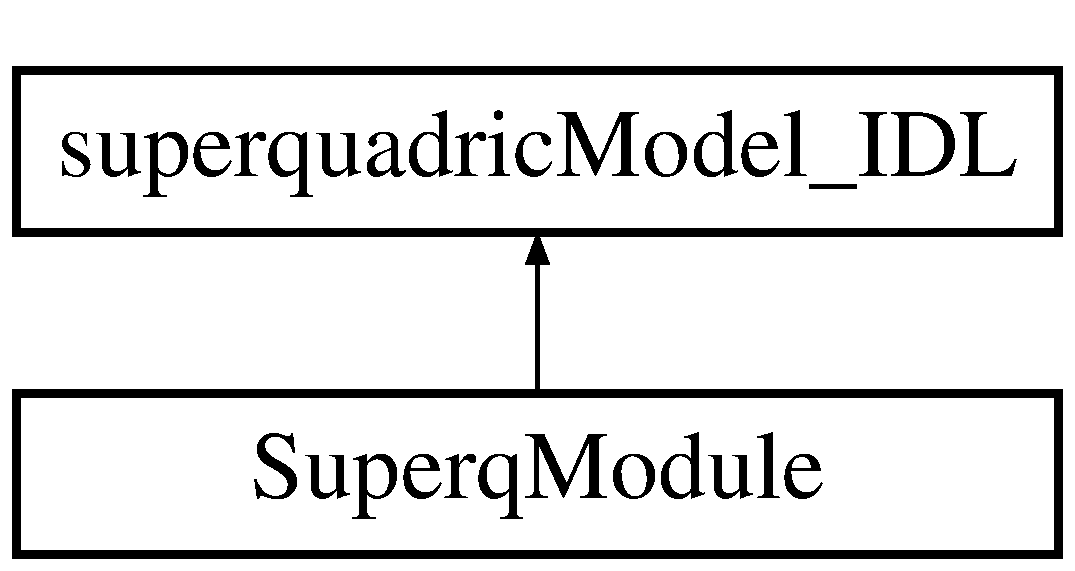
\includegraphics[height=2.000000cm]{classsuperquadricModel__IDL}
\end{center}
\end{figure}
\subsection*{Public Member Functions}
\begin{DoxyCompactItemize}
\item 
virtual bool \mbox{\hyperlink{classsuperquadricModel__IDL_a781426bfc4862e87ef75a4bbbfa33275}{set\+\_\+tag\+\_\+file}} (const std\+::string \&entry)
\begin{DoxyCompactList}\small\item\em Set the tag for storing files. \end{DoxyCompactList}\item 
virtual std\+::string \mbox{\hyperlink{classsuperquadricModel__IDL_a6d39eaa247aec65fe2bfefbdace4ec85}{get\+\_\+tag\+\_\+file}} ()
\begin{DoxyCompactList}\small\item\em Return the tag used for storing files. \end{DoxyCompactList}\item 
virtual yarp\+::os\+::\+Property \mbox{\hyperlink{classsuperquadricModel__IDL_a10039bb93445066d9dd29d8f6c9ef6c5}{get\+\_\+superq}} (const std\+::vector$<$ yarp\+::sig\+::\+Vector $>$ \&point\+\_\+cloud, const bool filtered\+\_\+or\+\_\+not, const bool reset\+\_\+or\+\_\+not)
\begin{DoxyCompactList}\small\item\em Get the parameters of the reconstructed superquadric. \end{DoxyCompactList}\item 
virtual bool \mbox{\hyperlink{classsuperquadricModel__IDL_a1a2080d797a81b46b0dffa86b5367e15}{set\+\_\+points\+\_\+filtering}} (const std\+::string \&entry)
\begin{DoxyCompactList}\small\item\em On/off point cloud filtering. \end{DoxyCompactList}\item 
virtual std\+::string \mbox{\hyperlink{classsuperquadricModel__IDL_aa490ebcf39414aaaae41d5095267abb9}{get\+\_\+points\+\_\+filtering}} ()
\begin{DoxyCompactList}\small\item\em Say if points filtering is on or not. \end{DoxyCompactList}\item 
virtual bool \mbox{\hyperlink{classsuperquadricModel__IDL_af418edf09afd9374c5272d018c58e8a7}{set\+\_\+superq\+\_\+filtering}} (const std\+::string \&entry)
\begin{DoxyCompactList}\small\item\em On/off superquadric filtering. \end{DoxyCompactList}\item 
virtual std\+::string \mbox{\hyperlink{classsuperquadricModel__IDL_af99d29d42b96b8db6c90c5fd48cfb253}{get\+\_\+superq\+\_\+filtering}} ()
\begin{DoxyCompactList}\small\item\em Say if superquadric filtering is on or not. \end{DoxyCompactList}\item 
virtual bool \mbox{\hyperlink{classsuperquadricModel__IDL_a8368b783845a3e5ae7e0706ee5b888c0}{set\+\_\+save\+\_\+points}} (const std\+::string \&entry)
\begin{DoxyCompactList}\small\item\em Set if you want to save the acquired point cloud. \end{DoxyCompactList}\item 
virtual std\+::string \mbox{\hyperlink{classsuperquadricModel__IDL_a4b101fe118a1ee912468562bde0b0df4}{get\+\_\+save\+\_\+points}} ()
\begin{DoxyCompactList}\small\item\em Set if you are saving the acquired point cloud. \end{DoxyCompactList}\item 
virtual yarp\+::os\+::\+Property \mbox{\hyperlink{classsuperquadricModel__IDL_a50b388a29852f9d8b57a0bbb276d4675}{get\+\_\+options}} (const std\+::string \&field)
\begin{DoxyCompactList}\small\item\em Get the parameters of the module. \end{DoxyCompactList}\item 
virtual bool \mbox{\hyperlink{classsuperquadricModel__IDL_a575e0b591f07206b0d6c29e5cfeead37}{set\+\_\+options}} (const yarp\+::os\+::\+Property \&options, const std\+::string \&field)
\begin{DoxyCompactList}\small\item\em Set the parameters of the module. \end{DoxyCompactList}\item 
virtual bool \mbox{\hyperlink{classsuperquadricModel__IDL_a651c741e9b01b25d46be96b06b91011d}{set\+\_\+visualization}} (const std\+::string \&e)
\begin{DoxyCompactList}\small\item\em Set if the visualization has to be enabled. \end{DoxyCompactList}\item 
virtual std\+::string \mbox{\hyperlink{classsuperquadricModel__IDL_a5d9f4f0622ba19b60218636dc108ef61}{get\+\_\+visualization}} ()
\begin{DoxyCompactList}\small\item\em Get if visualization is enabled. \end{DoxyCompactList}\item 
\mbox{\label{classsuperquadricModel__IDL_ac72a24dddca13978d7adcd5cf4f40b1f}} 
virtual bool {\bfseries read} (yarp\+::os\+::\+Connection\+Reader \&connection)
\item 
\mbox{\label{classsuperquadricModel__IDL_a263ca3dc1c7a21cc3ac40caadc95cf3d}} 
virtual std\+::vector$<$ std\+::string $>$ {\bfseries help} (const std\+::string \&function\+Name=\char`\"{}-\/-\/all\char`\"{})
\end{DoxyCompactItemize}


\subsection{Detailed Description}
\mbox{\hyperlink{classsuperquadricModel__IDL}{superquadric\+Model\+\_\+\+I\+DL}} I\+DL Interface to \mbox{\hyperlink{group__superquadric-model}{superquadric-\/model}} services. 

Definition at line 19 of file superquadric\+Model\+\_\+\+I\+D\+L.\+h.



\subsection{Member Function Documentation}
\mbox{\label{classsuperquadricModel__IDL_a50b388a29852f9d8b57a0bbb276d4675}} 
\index{superquadric\+Model\+\_\+\+I\+DL@{superquadric\+Model\+\_\+\+I\+DL}!get\+\_\+options@{get\+\_\+options}}
\index{get\+\_\+options@{get\+\_\+options}!superquadric\+Model\+\_\+\+I\+DL@{superquadric\+Model\+\_\+\+I\+DL}}
\subsubsection{\texorpdfstring{get\+\_\+options()}{get\_options()}}
{\footnotesize\ttfamily virtual yarp\+::os\+::\+Property superquadric\+Model\+\_\+\+I\+D\+L\+::get\+\_\+options (\begin{DoxyParamCaption}\item[{const std\+::string \&}]{field }\end{DoxyParamCaption})\hspace{0.3cm}{\ttfamily [virtual]}}



Get the parameters of the module. 

The user must pay attention in changing them. 
\begin{DoxyParams}{Parameters}
{\em field} & can be \char`\"{}points\+\_\+filter\char`\"{}, \char`\"{}superq\+\_\+filter\char`\"{}, \char`\"{}optimization\char`\"{}, \char`\"{}visualization\char`\"{} or \char`\"{}statistics\char`\"{}. depending on which parameters we are interested in. \\
\hline
\end{DoxyParams}
\begin{DoxyReturn}{Returns}
the Property including all the parameter values. 
\end{DoxyReturn}


Reimplemented in \mbox{\hyperlink{classSuperqModule_a18822e0a99dc0b13479f20960c577fb9}{Superq\+Module}}.

\mbox{\label{classsuperquadricModel__IDL_aa490ebcf39414aaaae41d5095267abb9}} 
\index{superquadric\+Model\+\_\+\+I\+DL@{superquadric\+Model\+\_\+\+I\+DL}!get\+\_\+points\+\_\+filtering@{get\+\_\+points\+\_\+filtering}}
\index{get\+\_\+points\+\_\+filtering@{get\+\_\+points\+\_\+filtering}!superquadric\+Model\+\_\+\+I\+DL@{superquadric\+Model\+\_\+\+I\+DL}}
\subsubsection{\texorpdfstring{get\+\_\+points\+\_\+filtering()}{get\_points\_filtering()}}
{\footnotesize\ttfamily virtual std\+::string superquadric\+Model\+\_\+\+I\+D\+L\+::get\+\_\+points\+\_\+filtering (\begin{DoxyParamCaption}{ }\end{DoxyParamCaption})\hspace{0.3cm}{\ttfamily [virtual]}}



Say if points filtering is on or not. 

\begin{DoxyReturn}{Returns}
on/off string if points filtering is on/off. 
\end{DoxyReturn}


Reimplemented in \mbox{\hyperlink{classSuperqModule_a60c8ff17436cc55a3e9b704dd6c2529b}{Superq\+Module}}.

\mbox{\label{classsuperquadricModel__IDL_a4b101fe118a1ee912468562bde0b0df4}} 
\index{superquadric\+Model\+\_\+\+I\+DL@{superquadric\+Model\+\_\+\+I\+DL}!get\+\_\+save\+\_\+points@{get\+\_\+save\+\_\+points}}
\index{get\+\_\+save\+\_\+points@{get\+\_\+save\+\_\+points}!superquadric\+Model\+\_\+\+I\+DL@{superquadric\+Model\+\_\+\+I\+DL}}
\subsubsection{\texorpdfstring{get\+\_\+save\+\_\+points()}{get\_save\_points()}}
{\footnotesize\ttfamily virtual std\+::string superquadric\+Model\+\_\+\+I\+D\+L\+::get\+\_\+save\+\_\+points (\begin{DoxyParamCaption}{ }\end{DoxyParamCaption})\hspace{0.3cm}{\ttfamily [virtual]}}



Set if you are saving the acquired point cloud. 

\begin{DoxyReturn}{Returns}
\char`\"{}on\char`\"{} or \char`\"{}off\char`\"{}. 
\end{DoxyReturn}


Reimplemented in \mbox{\hyperlink{classSuperqModule_adfeeea091edd0d32d388b072f4fc9d93}{Superq\+Module}}.

\mbox{\label{classsuperquadricModel__IDL_a10039bb93445066d9dd29d8f6c9ef6c5}} 
\index{superquadric\+Model\+\_\+\+I\+DL@{superquadric\+Model\+\_\+\+I\+DL}!get\+\_\+superq@{get\+\_\+superq}}
\index{get\+\_\+superq@{get\+\_\+superq}!superquadric\+Model\+\_\+\+I\+DL@{superquadric\+Model\+\_\+\+I\+DL}}
\subsubsection{\texorpdfstring{get\+\_\+superq()}{get\_superq()}}
{\footnotesize\ttfamily virtual yarp\+::os\+::\+Property superquadric\+Model\+\_\+\+I\+D\+L\+::get\+\_\+superq (\begin{DoxyParamCaption}\item[{const std\+::vector$<$ yarp\+::sig\+::\+Vector $>$ \&}]{point\+\_\+cloud,  }\item[{const bool}]{filtered\+\_\+or\+\_\+not,  }\item[{const bool}]{reset\+\_\+or\+\_\+not }\end{DoxyParamCaption})\hspace{0.3cm}{\ttfamily [virtual]}}



Get the parameters of the reconstructed superquadric. 


\begin{DoxyParams}{Parameters}
{\em point\+\_\+cloud} & is the 3D point cloud of the object we want to model with the superquadric, for instance\+: ((100.\+0 102.\+0) (100.\+0 103.\+0) ... ). \\
\hline
{\em filtered\+\_\+or\+\_\+not} & is a bool variable specifing if we want the superquadric to be filtered (true/1) or not (false/0). \\
\hline
{\em reset\+\_\+or\+\_\+not} & is a bool variable specifing if we want to reset the superquadric filtered (if enabled) or not. \\
\hline
\end{DoxyParams}
\begin{DoxyReturn}{Returns}
the 12 parameters (x0, .. x11) of the current superquadric. In particular, the parameters are grouped in a Property as follows\+: \char`\"{}dimensions\char`\"{} (x0, x1, x2) are the three semi-\/axes lenghts; \char`\"{}exponents\char`\"{} (x3 and x4) are the exponents, responsible for the superquadric shape; \char`\"{}center\char`\"{}(x5, x6, x7) contains the coordinate of the superquadric center; and \char`\"{}orientation\char`\"{} (x8, x9, 10, x11) is the axis-\/angle representation obtained from the Euler angles. 
\end{DoxyReturn}
\mbox{\label{classsuperquadricModel__IDL_af99d29d42b96b8db6c90c5fd48cfb253}} 
\index{superquadric\+Model\+\_\+\+I\+DL@{superquadric\+Model\+\_\+\+I\+DL}!get\+\_\+superq\+\_\+filtering@{get\+\_\+superq\+\_\+filtering}}
\index{get\+\_\+superq\+\_\+filtering@{get\+\_\+superq\+\_\+filtering}!superquadric\+Model\+\_\+\+I\+DL@{superquadric\+Model\+\_\+\+I\+DL}}
\subsubsection{\texorpdfstring{get\+\_\+superq\+\_\+filtering()}{get\_superq\_filtering()}}
{\footnotesize\ttfamily virtual std\+::string superquadric\+Model\+\_\+\+I\+D\+L\+::get\+\_\+superq\+\_\+filtering (\begin{DoxyParamCaption}{ }\end{DoxyParamCaption})\hspace{0.3cm}{\ttfamily [virtual]}}



Say if superquadric filtering is on or not. 

\begin{DoxyReturn}{Returns}
on/off string if superquadeic filtering is on/off. 
\end{DoxyReturn}


Reimplemented in \mbox{\hyperlink{classSuperqModule_a66cb1b371b92687d851b5ca23174198b}{Superq\+Module}}.

\mbox{\label{classsuperquadricModel__IDL_a6d39eaa247aec65fe2bfefbdace4ec85}} 
\index{superquadric\+Model\+\_\+\+I\+DL@{superquadric\+Model\+\_\+\+I\+DL}!get\+\_\+tag\+\_\+file@{get\+\_\+tag\+\_\+file}}
\index{get\+\_\+tag\+\_\+file@{get\+\_\+tag\+\_\+file}!superquadric\+Model\+\_\+\+I\+DL@{superquadric\+Model\+\_\+\+I\+DL}}
\subsubsection{\texorpdfstring{get\+\_\+tag\+\_\+file()}{get\_tag\_file()}}
{\footnotesize\ttfamily virtual std\+::string superquadric\+Model\+\_\+\+I\+D\+L\+::get\+\_\+tag\+\_\+file (\begin{DoxyParamCaption}{ }\end{DoxyParamCaption})\hspace{0.3cm}{\ttfamily [virtual]}}



Return the tag used for storing files. 

\begin{DoxyReturn}{Returns}
the tag name. 
\end{DoxyReturn}


Reimplemented in \mbox{\hyperlink{classSuperqModule_ac5475155a5a1b05e5fdef54699cef1a6}{Superq\+Module}}.

\mbox{\label{classsuperquadricModel__IDL_a5d9f4f0622ba19b60218636dc108ef61}} 
\index{superquadric\+Model\+\_\+\+I\+DL@{superquadric\+Model\+\_\+\+I\+DL}!get\+\_\+visualization@{get\+\_\+visualization}}
\index{get\+\_\+visualization@{get\+\_\+visualization}!superquadric\+Model\+\_\+\+I\+DL@{superquadric\+Model\+\_\+\+I\+DL}}
\subsubsection{\texorpdfstring{get\+\_\+visualization()}{get\_visualization()}}
{\footnotesize\ttfamily virtual std\+::string superquadric\+Model\+\_\+\+I\+D\+L\+::get\+\_\+visualization (\begin{DoxyParamCaption}{ }\end{DoxyParamCaption})\hspace{0.3cm}{\ttfamily [virtual]}}



Get if visualization is enabled. 

\begin{DoxyReturn}{Returns}
\char`\"{}on\char`\"{} or \char`\"{}off\char`\"{}. 
\end{DoxyReturn}


Reimplemented in \mbox{\hyperlink{classSuperqModule_a89be4778051c4dd19339021448f89b41}{Superq\+Module}}.

\mbox{\label{classsuperquadricModel__IDL_a575e0b591f07206b0d6c29e5cfeead37}} 
\index{superquadric\+Model\+\_\+\+I\+DL@{superquadric\+Model\+\_\+\+I\+DL}!set\+\_\+options@{set\+\_\+options}}
\index{set\+\_\+options@{set\+\_\+options}!superquadric\+Model\+\_\+\+I\+DL@{superquadric\+Model\+\_\+\+I\+DL}}
\subsubsection{\texorpdfstring{set\+\_\+options()}{set\_options()}}
{\footnotesize\ttfamily virtual bool superquadric\+Model\+\_\+\+I\+D\+L\+::set\+\_\+options (\begin{DoxyParamCaption}\item[{const yarp\+::os\+::\+Property \&}]{options,  }\item[{const std\+::string \&}]{field }\end{DoxyParamCaption})\hspace{0.3cm}{\ttfamily [virtual]}}



Set the parameters of the module. 

The user must pay attention in changing them. 
\begin{DoxyParams}{Parameters}
{\em options} & is a Property containing the parameters the user want to change. \\
\hline
{\em field} & is a string specifying which can of parameter we are going to change. Field can be\+: \char`\"{}points\+\_\+filter\char`\"{}, \char`\"{}superq\+\_\+filter\char`\"{}, \char`\"{}optimization\char`\"{} or \char`\"{}visualization\char`\"{}. You can set the parameters typing\+: command\+: set\+\_\+options ((filter\+\_\+radius $<$radius-\/value$>$) (filter\+\_\+nn\+Threshold $<$nn\+Threshold-\/value$>$)) points\+\_\+filter. \\
\hline
\end{DoxyParams}
\begin{DoxyReturn}{Returns}
true/false on success/failure. 
\end{DoxyReturn}


Reimplemented in \mbox{\hyperlink{classSuperqModule_a32ccf59ac0572ca77883237dd2d12890}{Superq\+Module}}.

\mbox{\label{classsuperquadricModel__IDL_a1a2080d797a81b46b0dffa86b5367e15}} 
\index{superquadric\+Model\+\_\+\+I\+DL@{superquadric\+Model\+\_\+\+I\+DL}!set\+\_\+points\+\_\+filtering@{set\+\_\+points\+\_\+filtering}}
\index{set\+\_\+points\+\_\+filtering@{set\+\_\+points\+\_\+filtering}!superquadric\+Model\+\_\+\+I\+DL@{superquadric\+Model\+\_\+\+I\+DL}}
\subsubsection{\texorpdfstring{set\+\_\+points\+\_\+filtering()}{set\_points\_filtering()}}
{\footnotesize\ttfamily virtual bool superquadric\+Model\+\_\+\+I\+D\+L\+::set\+\_\+points\+\_\+filtering (\begin{DoxyParamCaption}\item[{const std\+::string \&}]{entry }\end{DoxyParamCaption})\hspace{0.3cm}{\ttfamily [virtual]}}



On/off point cloud filtering. 


\begin{DoxyParams}{Parameters}
{\em entry} & is \char`\"{}on/off\char`\"{} if you want/do not want to filter points. \\
\hline
\end{DoxyParams}
\begin{DoxyReturn}{Returns}
true/false on success/failure. 
\end{DoxyReturn}


Reimplemented in \mbox{\hyperlink{classSuperqModule_a408203d0119443fb61544f84dafff8a4}{Superq\+Module}}.

\mbox{\label{classsuperquadricModel__IDL_a8368b783845a3e5ae7e0706ee5b888c0}} 
\index{superquadric\+Model\+\_\+\+I\+DL@{superquadric\+Model\+\_\+\+I\+DL}!set\+\_\+save\+\_\+points@{set\+\_\+save\+\_\+points}}
\index{set\+\_\+save\+\_\+points@{set\+\_\+save\+\_\+points}!superquadric\+Model\+\_\+\+I\+DL@{superquadric\+Model\+\_\+\+I\+DL}}
\subsubsection{\texorpdfstring{set\+\_\+save\+\_\+points()}{set\_save\_points()}}
{\footnotesize\ttfamily virtual bool superquadric\+Model\+\_\+\+I\+D\+L\+::set\+\_\+save\+\_\+points (\begin{DoxyParamCaption}\item[{const std\+::string \&}]{entry }\end{DoxyParamCaption})\hspace{0.3cm}{\ttfamily [virtual]}}



Set if you want to save the acquired point cloud. 


\begin{DoxyParams}{Parameters}
{\em entry} & can be\+: \char`\"{}on\char`\"{} or \char`\"{}off\char`\"{}. \\
\hline
\end{DoxyParams}
\begin{DoxyReturn}{Returns}
true/false on success/failure. 
\end{DoxyReturn}


Reimplemented in \mbox{\hyperlink{classSuperqModule_a90826fc53859ecf126f22a2569611b2c}{Superq\+Module}}.

\mbox{\label{classsuperquadricModel__IDL_af418edf09afd9374c5272d018c58e8a7}} 
\index{superquadric\+Model\+\_\+\+I\+DL@{superquadric\+Model\+\_\+\+I\+DL}!set\+\_\+superq\+\_\+filtering@{set\+\_\+superq\+\_\+filtering}}
\index{set\+\_\+superq\+\_\+filtering@{set\+\_\+superq\+\_\+filtering}!superquadric\+Model\+\_\+\+I\+DL@{superquadric\+Model\+\_\+\+I\+DL}}
\subsubsection{\texorpdfstring{set\+\_\+superq\+\_\+filtering()}{set\_superq\_filtering()}}
{\footnotesize\ttfamily virtual bool superquadric\+Model\+\_\+\+I\+D\+L\+::set\+\_\+superq\+\_\+filtering (\begin{DoxyParamCaption}\item[{const std\+::string \&}]{entry }\end{DoxyParamCaption})\hspace{0.3cm}{\ttfamily [virtual]}}



On/off superquadric filtering. 


\begin{DoxyParams}{Parameters}
{\em entry} & is \char`\"{}on/off\char`\"{} if you want/do not want to filter the estimated superquadric. \\
\hline
\end{DoxyParams}
\begin{DoxyReturn}{Returns}
true/false on success/failure. 
\end{DoxyReturn}


Reimplemented in \mbox{\hyperlink{classSuperqModule_a902d4a48d1a919ff9d9b1f7d1c132577}{Superq\+Module}}.

\mbox{\label{classsuperquadricModel__IDL_a781426bfc4862e87ef75a4bbbfa33275}} 
\index{superquadric\+Model\+\_\+\+I\+DL@{superquadric\+Model\+\_\+\+I\+DL}!set\+\_\+tag\+\_\+file@{set\+\_\+tag\+\_\+file}}
\index{set\+\_\+tag\+\_\+file@{set\+\_\+tag\+\_\+file}!superquadric\+Model\+\_\+\+I\+DL@{superquadric\+Model\+\_\+\+I\+DL}}
\subsubsection{\texorpdfstring{set\+\_\+tag\+\_\+file()}{set\_tag\_file()}}
{\footnotesize\ttfamily virtual bool superquadric\+Model\+\_\+\+I\+D\+L\+::set\+\_\+tag\+\_\+file (\begin{DoxyParamCaption}\item[{const std\+::string \&}]{entry }\end{DoxyParamCaption})\hspace{0.3cm}{\ttfamily [virtual]}}



Set the tag for storing files. 


\begin{DoxyParams}{Parameters}
{\em entry} & is the tag that will be used in file names. \\
\hline
\end{DoxyParams}
\begin{DoxyReturn}{Returns}
true. 
\end{DoxyReturn}


Reimplemented in \mbox{\hyperlink{classSuperqModule_ae9f0cfead2c367e4c3aa25292b5c42c6}{Superq\+Module}}.

\mbox{\label{classsuperquadricModel__IDL_a651c741e9b01b25d46be96b06b91011d}} 
\index{superquadric\+Model\+\_\+\+I\+DL@{superquadric\+Model\+\_\+\+I\+DL}!set\+\_\+visualization@{set\+\_\+visualization}}
\index{set\+\_\+visualization@{set\+\_\+visualization}!superquadric\+Model\+\_\+\+I\+DL@{superquadric\+Model\+\_\+\+I\+DL}}
\subsubsection{\texorpdfstring{set\+\_\+visualization()}{set\_visualization()}}
{\footnotesize\ttfamily virtual bool superquadric\+Model\+\_\+\+I\+D\+L\+::set\+\_\+visualization (\begin{DoxyParamCaption}\item[{const std\+::string \&}]{e }\end{DoxyParamCaption})\hspace{0.3cm}{\ttfamily [virtual]}}



Set if the visualization has to be enabled. 

\begin{DoxyReturn}{Returns}
true/false on success/failure. 
\end{DoxyReturn}


Reimplemented in \mbox{\hyperlink{classSuperqModule_ae4fc54ad89b3ee72ab5ea8c8b5065866}{Superq\+Module}}.



The documentation for this class was generated from the following file\+:\begin{DoxyCompactItemize}
\item 
C\+:/\+Users/upattacini/\+Desktop/superquadric-\/model/idl\+\_\+dox/superquadric\+Model\+\_\+\+I\+D\+L.\+h\end{DoxyCompactItemize}

\section{Superq\+Visualization Class Reference}
\label{classSuperqVisualization}\index{Superq\+Visualization@{Superq\+Visualization}}


This class shows the point cloud used for modeling or the estimated superquadric overlapped on the camera image and in real time.  




{\ttfamily \#include $<$superq\+Visualization.\+h$>$}



Inherits Rate\+Thread.

\subsection*{Public Member Functions}
\begin{DoxyCompactItemize}
\item 
\mbox{\label{classSuperqVisualization_ac387ba6f204a820657e399cedbe84d43}} 
{\bfseries Superq\+Visualization} (int rate, const std\+::string \&\+\_\+eye, const std\+::string \&\+\_\+what\+\_\+to\+\_\+plot, yarp\+::sig\+::\+Vector \&\+\_\+x, yarp\+::sig\+::\+Vector \&\+\_\+x\+\_\+filtered, std\+::deque$<$ int $>$ \&\+\_\+\+Color, yarp\+::dev\+::\+I\+Gaze\+Control $\ast$\+\_\+igaze, const yarp\+::sig\+::\+Matrix \+\_\+K, std\+::deque$<$ yarp\+::sig\+::\+Vector $>$ \&\+\_\+points, const int \&\+\_\+vis\+\_\+points, const int \&\+\_\+vis\+\_\+step)
\item 
bool \mbox{\hyperlink{classSuperqVisualization_aea374f59e3b941e688c1ddafad8896b9}{show\+Points}} ()
\begin{DoxyCompactList}\small\item\em Show point cloud on the image. \end{DoxyCompactList}\item 
bool \mbox{\hyperlink{classSuperqVisualization_aa763f8f73c82d4de1d47b03ae9d2e276}{show\+Superq}} (yarp\+::sig\+::\+Vector \&x\+\_\+to\+\_\+show)
\begin{DoxyCompactList}\small\item\em Show reconstructed superquadric on the image. \end{DoxyCompactList}\item 
yarp\+::sig\+::\+Vector \mbox{\hyperlink{classSuperqVisualization_aff405a4d0ad916decad09f923e319be6}{from3\+Dto2D}} (const yarp\+::sig\+::\+Vector \&point3D)
\begin{DoxyCompactList}\small\item\em Compute 2D pixels from 3D points. \end{DoxyCompactList}\item 
\mbox{\label{classSuperqVisualization_a93dc1583d46a71bbcc4e4ef7f65820b9}} 
virtual bool \mbox{\hyperlink{classSuperqVisualization_a93dc1583d46a71bbcc4e4ef7f65820b9}{thread\+Init}} ()
\begin{DoxyCompactList}\small\item\em Init function of Rate\+Thread. \end{DoxyCompactList}\item 
\mbox{\label{classSuperqVisualization_a46d689c65cec6c04d3fffdbfbbd1838b}} 
virtual void \mbox{\hyperlink{classSuperqVisualization_a46d689c65cec6c04d3fffdbfbbd1838b}{run}} ()
\begin{DoxyCompactList}\small\item\em Run function of Rate\+Thread. \end{DoxyCompactList}\item 
\mbox{\label{classSuperqVisualization_a0fceb3fcc3bd4eadbf9d68abb4b0badc}} 
void \mbox{\hyperlink{classSuperqVisualization_a0fceb3fcc3bd4eadbf9d68abb4b0badc}{interrupt\+Ports}} ()
\begin{DoxyCompactList}\small\item\em Interrupt ports functionalities. \end{DoxyCompactList}\item 
\mbox{\label{classSuperqVisualization_ae79d791d2accf581cbe0502d579f5416}} 
virtual void \mbox{\hyperlink{classSuperqVisualization_ae79d791d2accf581cbe0502d579f5416}{thread\+Release}} ()
\begin{DoxyCompactList}\small\item\em Release function of Rate\+Thread. \end{DoxyCompactList}\item 
void \mbox{\hyperlink{classSuperqVisualization_acbc374ffecb809ca16853c9475d7f347}{set\+Par}} (const std\+::string \&par\+\_\+name, const std\+::string \&value)
\begin{DoxyCompactList}\small\item\em Set a given parameter equal to a string. \end{DoxyCompactList}\item 
void \mbox{\hyperlink{classSuperqVisualization_a2403b8fcb9448e61866fd39035a482f0}{set\+Par}} (const std\+::string \&par\+\_\+name, const int \&value)
\begin{DoxyCompactList}\small\item\em Set a given parameter equal to a desired value. \end{DoxyCompactList}\item 
void \mbox{\hyperlink{classSuperqVisualization_a82eb6b92c07720b35c714a3c8e2f88a3}{set\+Color}} (const int \&\mbox{\hyperlink{classSuperqVisualization_aee081a694340a9a8658a960872cb6172}{r}}, const int \&\mbox{\hyperlink{classSuperqVisualization_a51cc6e3ac3ee243250a7042f00c813d1}{g}}, const int \&\mbox{\hyperlink{classSuperqVisualization_a96c39287f863466bbbc21342dd62b68a}{b}})
\begin{DoxyCompactList}\small\item\em Set color for visualization. \end{DoxyCompactList}\item 
void \mbox{\hyperlink{classSuperqVisualization_a5250a90e5865bf45c0bd8ae919b8eab0}{set\+Par}} (const yarp\+::os\+::\+Property \&new\+Options, bool first\+\_\+time)
\begin{DoxyCompactList}\small\item\em Set parameters for visualization. \end{DoxyCompactList}\item 
yarp\+::os\+::\+Property \mbox{\hyperlink{classSuperqVisualization_ae4fac8f79629a3fa81a688ab4baf61f7}{get\+Par}} ()
\begin{DoxyCompactList}\small\item\em Get parameters for visualization. \end{DoxyCompactList}\item 
double \mbox{\hyperlink{classSuperqVisualization_a9583b378f68f466a76022817d3051c6e}{get\+Time}} ()
\begin{DoxyCompactList}\small\item\em Get time required for visualization. \end{DoxyCompactList}\end{DoxyCompactItemize}
\subsection*{Data Fields}
\begin{DoxyCompactItemize}
\item 
\mbox{\label{classSuperqVisualization_a57358b13afc9b5aa3920b7c96b20b26d}} 
yarp\+::sig\+::\+Vector \& \mbox{\hyperlink{classSuperqVisualization_a57358b13afc9b5aa3920b7c96b20b26d}{superq}}
\begin{DoxyCompactList}\small\item\em Estimated superquadric. \end{DoxyCompactList}\item 
\mbox{\label{classSuperqVisualization_aed6197ba510529ed07d32a1a86a48e83}} 
yarp\+::sig\+::\+Vector \& \mbox{\hyperlink{classSuperqVisualization_aed6197ba510529ed07d32a1a86a48e83}{superq\+\_\+filtered}}
\begin{DoxyCompactList}\small\item\em Filtered superquadric. \end{DoxyCompactList}\item 
\mbox{\label{classSuperqVisualization_aa00fb7590a7bc410387e041fbdfb162a}} 
std\+::deque$<$ yarp\+::sig\+::\+Vector $>$ \& \mbox{\hyperlink{classSuperqVisualization_aa00fb7590a7bc410387e041fbdfb162a}{points}}
\begin{DoxyCompactList}\small\item\em Object point cloud. \end{DoxyCompactList}\item 
\mbox{\label{classSuperqVisualization_a599776b35fd931a41a9bf6416e639275}} 
yarp\+::sig\+::\+Image\+Of$<$ yarp\+::sig\+::\+Pixel\+Rgb $>$ $\ast$ \mbox{\hyperlink{classSuperqVisualization_a599776b35fd931a41a9bf6416e639275}{img\+In}}
\begin{DoxyCompactList}\small\item\em Input image. \end{DoxyCompactList}\end{DoxyCompactItemize}
\subsection*{Protected Attributes}
\begin{DoxyCompactItemize}
\item 
\mbox{\label{classSuperqVisualization_a567a3ef8af7cbd836fcd04c24c314243}} 
yarp\+::os\+::\+Buffered\+Port$<$ yarp\+::sig\+::\+Image\+Of$<$ yarp\+::sig\+::\+Pixel\+Rgb $>$ $>$ \mbox{\hyperlink{classSuperqVisualization_a567a3ef8af7cbd836fcd04c24c314243}{port\+Img\+In}}
\begin{DoxyCompactList}\small\item\em Input image port. \end{DoxyCompactList}\item 
\mbox{\label{classSuperqVisualization_a0ed5bf82e324579e781952b7a540d5c0}} 
yarp\+::os\+::\+Buffered\+Port$<$ yarp\+::sig\+::\+Image\+Of$<$ yarp\+::sig\+::\+Pixel\+Rgb $>$ $>$ \mbox{\hyperlink{classSuperqVisualization_a0ed5bf82e324579e781952b7a540d5c0}{port\+Img\+Out}}
\begin{DoxyCompactList}\small\item\em Output image port $\ast$. \end{DoxyCompactList}\item 
\mbox{\label{classSuperqVisualization_aee081a694340a9a8658a960872cb6172}} 
int \mbox{\hyperlink{classSuperqVisualization_aee081a694340a9a8658a960872cb6172}{r}}
\begin{DoxyCompactList}\small\item\em R value for visualization. \end{DoxyCompactList}\item 
\mbox{\label{classSuperqVisualization_a51cc6e3ac3ee243250a7042f00c813d1}} 
int \mbox{\hyperlink{classSuperqVisualization_a51cc6e3ac3ee243250a7042f00c813d1}{g}}
\begin{DoxyCompactList}\small\item\em Green value for visualization. \end{DoxyCompactList}\item 
\mbox{\label{classSuperqVisualization_a96c39287f863466bbbc21342dd62b68a}} 
int \mbox{\hyperlink{classSuperqVisualization_a96c39287f863466bbbc21342dd62b68a}{b}}
\begin{DoxyCompactList}\small\item\em Blue value for visualization. \end{DoxyCompactList}\item 
\mbox{\label{classSuperqVisualization_af984de33154bf4ebe0abf6f1f5047a1c}} 
double \mbox{\hyperlink{classSuperqVisualization_af984de33154bf4ebe0abf6f1f5047a1c}{t\+\_\+vis}}
\begin{DoxyCompactList}\small\item\em Time for visualization. \end{DoxyCompactList}\item 
\mbox{\label{classSuperqVisualization_a97eaa294a7c48033ef5695976556435a}} 
int \mbox{\hyperlink{classSuperqVisualization_a97eaa294a7c48033ef5695976556435a}{vis\+\_\+points}}
\begin{DoxyCompactList}\small\item\em Number of points used for visualization. \end{DoxyCompactList}\item 
\mbox{\label{classSuperqVisualization_a43a34e1d587532fbff246941cd28e3b6}} 
int \mbox{\hyperlink{classSuperqVisualization_a43a34e1d587532fbff246941cd28e3b6}{vis\+\_\+step}}
\begin{DoxyCompactList}\small\item\em Number of visualization step. \end{DoxyCompactList}\item 
\mbox{\label{classSuperqVisualization_a60f1dd2489b897777edffc4dfdebe64d}} 
std\+::string \mbox{\hyperlink{classSuperqVisualization_a60f1dd2489b897777edffc4dfdebe64d}{what\+\_\+to\+\_\+plot}}
\begin{DoxyCompactList}\small\item\em String used for deciding what to plot\+: \char`\"{}points\char`\"{} or \char`\"{}superq\char`\"{}. \end{DoxyCompactList}\item 
\mbox{\label{classSuperqVisualization_a77fbae5c4996f393cae867d56cf2ee16}} 
yarp\+::sig\+::\+Vector {\bfseries point}
\item 
\mbox{\label{classSuperqVisualization_a43a15830ead614d6962ac4777c8fc014}} 
yarp\+::sig\+::\+Vector {\bfseries point1}
\item 
\mbox{\label{classSuperqVisualization_a186ba8f98b1344934bab2fc2de516375}} 
yarp\+::sig\+::\+Vector {\bfseries point2D}
\item 
\mbox{\label{classSuperqVisualization_ae976f619addaebdf724316f25e2c38a8}} 
std\+::deque$<$ int $>$ {\bfseries Color}
\item 
\mbox{\label{classSuperqVisualization_a57cd2c0f68d9bf7365b8c9334b7c07bd}} 
std\+::string \mbox{\hyperlink{classSuperqVisualization_a57cd2c0f68d9bf7365b8c9334b7c07bd}{eye}}
\begin{DoxyCompactList}\small\item\em Eye camera selected. \end{DoxyCompactList}\item 
\mbox{\label{classSuperqVisualization_ad38ada4dfaaf6ced81c6da9aacba4bc0}} 
yarp\+::sig\+::\+Matrix {\bfseries R}
\item 
\mbox{\label{classSuperqVisualization_a64d02e9b2b003bb30235522f1b293a59}} 
yarp\+::sig\+::\+Matrix {\bfseries H}
\item 
\mbox{\label{classSuperqVisualization_a3b44b49611b760f95341303143b72804}} 
yarp\+::sig\+::\+Matrix {\bfseries K}
\item 
\mbox{\label{classSuperqVisualization_a70393943f451663a458119c63b6e0ebf}} 
yarp\+::dev\+::\+I\+Gaze\+Control $\ast$ \mbox{\hyperlink{classSuperqVisualization_a70393943f451663a458119c63b6e0ebf}{igaze}}
\begin{DoxyCompactList}\small\item\em Gaze Control interface. \end{DoxyCompactList}\item 
\mbox{\label{classSuperqVisualization_a5925440ac066d2d7dd40df5758e76bbf}} 
yarp\+::os\+::\+Mutex {\bfseries mutex}
\end{DoxyCompactItemize}


\subsection{Detailed Description}
This class shows the point cloud used for modeling or the estimated superquadric overlapped on the camera image and in real time. 

Definition at line 36 of file superq\+Visualization.\+h.



\subsection{Member Function Documentation}
\mbox{\label{classSuperqVisualization_aff405a4d0ad916decad09f923e319be6}} 
\index{Superq\+Visualization@{Superq\+Visualization}!from3\+Dto2D@{from3\+Dto2D}}
\index{from3\+Dto2D@{from3\+Dto2D}!Superq\+Visualization@{Superq\+Visualization}}
\subsubsection{\texorpdfstring{from3\+Dto2\+D()}{from3Dto2D()}}
{\footnotesize\ttfamily Vector Superq\+Visualization\+::from3\+Dto2D (\begin{DoxyParamCaption}\item[{const yarp\+::sig\+::\+Vector \&}]{point3D }\end{DoxyParamCaption})}



Compute 2D pixels from 3D points. 


\begin{DoxyParams}{Parameters}
{\em point3D} & is the 3D point to be converted \\
\hline
\end{DoxyParams}
\begin{DoxyReturn}{Returns}
a 2D vector representing the corresponding pixel 
\end{DoxyReturn}


Definition at line 168 of file superq\+Visualization.\+cpp.



Referenced by show\+Points(), and show\+Superq().


\begin{DoxyCode}
169 \{
170     Vector point2D(3,0.0);
171     Vector point\_aux(4,1.0);
172     point\_aux.setSubvector(0,point3D);
173     point2D=K*H*point\_aux;
174     \textcolor{keywordflow}{return} point2D.subVector(0,1)/point2D[2];
175 \}
\end{DoxyCode}
\mbox{\label{classSuperqVisualization_ae4fac8f79629a3fa81a688ab4baf61f7}} 
\index{Superq\+Visualization@{Superq\+Visualization}!get\+Par@{get\+Par}}
\index{get\+Par@{get\+Par}!Superq\+Visualization@{Superq\+Visualization}}
\subsubsection{\texorpdfstring{get\+Par()}{getPar()}}
{\footnotesize\ttfamily Property Superq\+Visualization\+::get\+Par (\begin{DoxyParamCaption}{ }\end{DoxyParamCaption})}



Get parameters for visualization. 

\begin{DoxyReturn}{Returns}
a property with all the visualization options 
\end{DoxyReturn}


Definition at line 330 of file superq\+Visualization.\+cpp.



References eye, vis\+\_\+points, vis\+\_\+step, and what\+\_\+to\+\_\+plot.


\begin{DoxyCode}
331 \{
332     LockGuard lg(mutex);
333 
334     Property advOptions;
335     advOptions.put(\textcolor{stringliteral}{"visualized\_points"},vis_points);
336     \textcolor{keywordflow}{if} (Color[0]==255 && Color[1]==0 && Color[2]==0)
337         advOptions.put(\textcolor{stringliteral}{"color"},\textcolor{stringliteral}{"red"});
338     \textcolor{keywordflow}{else} \textcolor{keywordflow}{if}  (Color[0]==0 && Color[1]==255 && Color[2]==0)
339         advOptions.put(\textcolor{stringliteral}{"color"},\textcolor{stringliteral}{"green"});
340     \textcolor{keywordflow}{else} \textcolor{keywordflow}{if}  (Color[0]==0 && Color[1]==0 &&Color[2]==255)
341         advOptions.put(\textcolor{stringliteral}{"color"},\textcolor{stringliteral}{"blue"});
342     advOptions.put(\textcolor{stringliteral}{"camera"},eye);
343     advOptions.put(\textcolor{stringliteral}{"visualized\_points\_step"},vis_step);
344     advOptions.put(\textcolor{stringliteral}{"what\_to\_plot"},what_to_plot);
345     \textcolor{keywordflow}{return} advOptions;
346 \}
\end{DoxyCode}
\mbox{\label{classSuperqVisualization_a9583b378f68f466a76022817d3051c6e}} 
\index{Superq\+Visualization@{Superq\+Visualization}!get\+Time@{get\+Time}}
\index{get\+Time@{get\+Time}!Superq\+Visualization@{Superq\+Visualization}}
\subsubsection{\texorpdfstring{get\+Time()}{getTime()}}
{\footnotesize\ttfamily double Superq\+Visualization\+::get\+Time (\begin{DoxyParamCaption}{ }\end{DoxyParamCaption})}



Get time required for visualization. 

\begin{DoxyReturn}{Returns}
the visualization time 
\end{DoxyReturn}


Definition at line 349 of file superq\+Visualization.\+cpp.



References t\+\_\+vis.


\begin{DoxyCode}
350 \{   
351     LockGuard lg(mutex);
352     \textcolor{keywordflow}{return} t_vis;
353 \}
\end{DoxyCode}
\mbox{\label{classSuperqVisualization_a82eb6b92c07720b35c714a3c8e2f88a3}} 
\index{Superq\+Visualization@{Superq\+Visualization}!set\+Color@{set\+Color}}
\index{set\+Color@{set\+Color}!Superq\+Visualization@{Superq\+Visualization}}
\subsubsection{\texorpdfstring{set\+Color()}{setColor()}}
{\footnotesize\ttfamily void Superq\+Visualization\+::set\+Color (\begin{DoxyParamCaption}\item[{const int \&}]{r,  }\item[{const int \&}]{g,  }\item[{const int \&}]{b }\end{DoxyParamCaption})}



Set color for visualization. 


\begin{DoxyParams}{Parameters}
{\em r} & is the red component \\
\hline
{\em g} & is the green component \\
\hline
{\em b} & is the blue component \\
\hline
\end{DoxyParams}
\mbox{\label{classSuperqVisualization_acbc374ffecb809ca16853c9475d7f347}} 
\index{Superq\+Visualization@{Superq\+Visualization}!set\+Par@{set\+Par}}
\index{set\+Par@{set\+Par}!Superq\+Visualization@{Superq\+Visualization}}
\subsubsection{\texorpdfstring{set\+Par()}{setPar()}\hspace{0.1cm}{\footnotesize\ttfamily [1/3]}}
{\footnotesize\ttfamily void Superq\+Visualization\+::set\+Par (\begin{DoxyParamCaption}\item[{const std\+::string \&}]{par\+\_\+name,  }\item[{const std\+::string \&}]{value }\end{DoxyParamCaption})}



Set a given parameter equal to a string. 


\begin{DoxyParams}{Parameters}
{\em par\+\_\+name} & is the name of the parameter to be changed \\
\hline
{\em value} & is the new value \\
\hline
\end{DoxyParams}
\mbox{\label{classSuperqVisualization_a2403b8fcb9448e61866fd39035a482f0}} 
\index{Superq\+Visualization@{Superq\+Visualization}!set\+Par@{set\+Par}}
\index{set\+Par@{set\+Par}!Superq\+Visualization@{Superq\+Visualization}}
\subsubsection{\texorpdfstring{set\+Par()}{setPar()}\hspace{0.1cm}{\footnotesize\ttfamily [2/3]}}
{\footnotesize\ttfamily void Superq\+Visualization\+::set\+Par (\begin{DoxyParamCaption}\item[{const std\+::string \&}]{par\+\_\+name,  }\item[{const int \&}]{value }\end{DoxyParamCaption})}



Set a given parameter equal to a desired value. 


\begin{DoxyParams}{Parameters}
{\em par\+\_\+name} & is the name of the parameter to be changed \\
\hline
{\em value} & is the new value \\
\hline
\end{DoxyParams}
\mbox{\label{classSuperqVisualization_a5250a90e5865bf45c0bd8ae919b8eab0}} 
\index{Superq\+Visualization@{Superq\+Visualization}!set\+Par@{set\+Par}}
\index{set\+Par@{set\+Par}!Superq\+Visualization@{Superq\+Visualization}}
\subsubsection{\texorpdfstring{set\+Par()}{setPar()}\hspace{0.1cm}{\footnotesize\ttfamily [3/3]}}
{\footnotesize\ttfamily void Superq\+Visualization\+::set\+Par (\begin{DoxyParamCaption}\item[{const yarp\+::os\+::\+Property \&}]{new\+Options,  }\item[{bool}]{first\+\_\+time }\end{DoxyParamCaption})}



Set parameters for visualization. 


\begin{DoxyParams}{Parameters}
{\em new\+Options} & is a Property with the new options to set \\
\hline
{\em first\+\_\+time} & takes into account if the options have already been set or not \\
\hline
\end{DoxyParams}
\mbox{\label{classSuperqVisualization_aea374f59e3b941e688c1ddafad8896b9}} 
\index{Superq\+Visualization@{Superq\+Visualization}!show\+Points@{show\+Points}}
\index{show\+Points@{show\+Points}!Superq\+Visualization@{Superq\+Visualization}}
\subsubsection{\texorpdfstring{show\+Points()}{showPoints()}}
{\footnotesize\ttfamily bool Superq\+Visualization\+::show\+Points (\begin{DoxyParamCaption}{ }\end{DoxyParamCaption})}



Show point cloud on the image. 

\begin{DoxyReturn}{Returns}
true 
\end{DoxyReturn}


Definition at line 117 of file superq\+Visualization.\+cpp.



References eye, from3\+Dto2\+D(), igaze, img\+In, points, port\+Img\+Out, and vis\+\_\+step.



Referenced by run().


\begin{DoxyCode}
118 \{
119     PixelRgb color(Color[0],Color[1],Color[2]);
120     Stamp *stamp=NULL;
121     Vector pos, orient;
122 
123     ImageOf<PixelRgb> &imgOut=portImgOut.prepare();
124     imgOut=*imgIn;
125 
126     \textcolor{keywordflow}{if} (eye==\textcolor{stringliteral}{"left"})
127     \{
128         \textcolor{keywordflow}{if} (igaze->getLeftEyePose(pos,orient,stamp))
129         \{
130             H=axis2dcm(orient);
131             H.setSubcol(pos,0,3);
132             H=SE3inv(H);
133         \}
134     \}
135     \textcolor{keywordflow}{else}
136     \{
137         \textcolor{keywordflow}{if} (igaze->getRightEyePose(pos,orient,stamp))
138         \{
139             H=axis2dcm(orient);
140             H.setSubcol(pos,0,3);
141             H=SE3inv(H);
142         \}
143     \}
144 
145     Vector point(3,0.0);
146 
147      \textcolor{keywordflow}{for} (\textcolor{keywordtype}{size\_t} i=0; i<points.size(); i+=vis_step)
148      \{
149          point=points[i].subVector(0,2);
150          point2D=from3Dto2D(point);
151 
152          cv::Point target\_point((\textcolor{keywordtype}{int})point2D[0],(\textcolor{keywordtype}{int})point2D[1]);
153 
154          \textcolor{keywordflow}{if} ((target\_point.x<0) || (target\_point.y<0) || (target\_point.x>=320) || (target\_point.y>=240))
155          \{
156              yWarning(\textcolor{stringliteral}{"[SuperqVisualization]:  Not acceptable pixels!"});
157          \}
158          \textcolor{keywordflow}{else}
159             imgOut.pixel(target\_point.x, target\_point.y)=color;
160      \}
161 
162     portImgOut.write();
163 
164     \textcolor{keywordflow}{return} \textcolor{keyword}{true};
165 \}
\end{DoxyCode}
\mbox{\label{classSuperqVisualization_aa763f8f73c82d4de1d47b03ae9d2e276}} 
\index{Superq\+Visualization@{Superq\+Visualization}!show\+Superq@{show\+Superq}}
\index{show\+Superq@{show\+Superq}!Superq\+Visualization@{Superq\+Visualization}}
\subsubsection{\texorpdfstring{show\+Superq()}{showSuperq()}}
{\footnotesize\ttfamily bool Superq\+Visualization\+::show\+Superq (\begin{DoxyParamCaption}\item[{yarp\+::sig\+::\+Vector \&}]{x\+\_\+to\+\_\+show }\end{DoxyParamCaption})}



Show reconstructed superquadric on the image. 


\begin{DoxyParams}{Parameters}
{\em x\+\_\+to\+\_\+show} & is the superquadric to be shown \\
\hline
\end{DoxyParams}
\begin{DoxyReturn}{Returns}
true/false on success/failure 
\end{DoxyReturn}


Definition at line 39 of file superq\+Visualization.\+cpp.



References eye, from3\+Dto2\+D(), igaze, img\+In, port\+Img\+Out, and vis\+\_\+points.



Referenced by run().


\begin{DoxyCode}
40 \{
41     LockGuard lg(mutex);
42 
43     PixelRgb color(Color[0],Color[1],Color[2]);
44     Vector pos, orient;
45     \textcolor{keywordtype}{double} co,so,ce,se;
46     Stamp *stamp=NULL;
47 
48     ImageOf<PixelRgb> &imgOut=portImgOut.prepare();
49     imgOut=*imgIn;
50 
51     R=euler2dcm(x\_toshow.subVector(8,10));
52     R=R.transposed();
53 
54     \textcolor{keywordflow}{if} ((norm(x\_toshow)>0.0))
55     \{
56         \textcolor{keywordflow}{if} (eye==\textcolor{stringliteral}{"left"})
57         \{
58             \textcolor{keywordflow}{if} (igaze->getLeftEyePose(pos,orient,stamp))
59             \{
60                 H=axis2dcm(orient);
61                 H.setSubcol(pos,0,3);
62                 H=SE3inv(H);
63             \}
64         \}
65         \textcolor{keywordflow}{else}
66         \{
67             \textcolor{keywordflow}{if} (igaze->getRightEyePose(pos,orient,stamp))
68             \{
69                 H=axis2dcm(orient);
70                 H.setSubcol(pos,0,3);
71                 H=SE3inv(H);
72             \}
73         \}
74 
75         \textcolor{keywordtype}{double} step=2*M\_PI/vis_points;
76 
77         \textcolor{keywordflow}{for} (\textcolor{keywordtype}{double} eta=-M\_PI; eta<M\_PI; eta+=step)
78         \{
79              \textcolor{keywordflow}{for} (\textcolor{keywordtype}{double} omega=-M\_PI; omega<M\_PI;omega+=step)
80              \{
81                  co=cos(omega); so=sin(omega);
82                  ce=cos(eta); se=sin(eta);
83 
84                  point[0]=x\_toshow[0] * sign(ce)*(pow(abs(ce),x\_toshow[3])) * sign(co)*(pow(abs(co),
      x\_toshow[4])) * R(0,0) +
85                             x\_toshow[1] * sign(ce)*(pow(abs(ce),x\_toshow[3]))* sign(so)*(pow(abs(so),
      x\_toshow[4])) * R(0,1)+
86                                 x\_toshow[2] * sign(se)*(pow(abs(se),x\_toshow[3])) * R(0,2) + x\_toshow[5];
87 
88                  point[1]=x\_toshow[0] * sign(ce)*(pow(abs(ce),x\_toshow[3])) * sign(co)*(pow(abs(co),
      x\_toshow[4])) * R(1,0) +
89                             x\_toshow[1] * sign(ce)*(pow(abs(ce),x\_toshow[3])) * sign(so)*(pow(abs(so),
      x\_toshow[4])) * R(1,1)+
90                                 x\_toshow[2] * sign(se)*(pow(abs(se),x\_toshow[3])) * R(1,2) + x\_toshow[6];
91 
92                  point[2]=x\_toshow[0] * sign(ce)*(pow(abs(ce),x\_toshow[3])) * sign(co)*(pow(abs(co),
      x\_toshow[4])) * R(2,0) +
93                             x\_toshow[1] * sign(ce)*(pow(abs(ce),x\_toshow[3])) * sign(so)*(pow(abs(so),
      x\_toshow[4])) * R(2,1)+
94                                 x\_toshow[2] * sign(se)*(pow(abs(se),x\_toshow[3])) * R(2,2) + x\_toshow[7];
95 
96                  point2D=from3Dto2D(point);
97 
98                  cv::Point target\_point((\textcolor{keywordtype}{int})point2D[0],(\textcolor{keywordtype}{int})point2D[1]);
99 
100                  \textcolor{keywordflow}{if} ((target\_point.x<0) || (target\_point.y<0) || (target\_point.x>=320) || (target\_point.y>=
      240))
101                  \{
102                      yWarning(\textcolor{stringliteral}{"[SuperqVisualization]: Not acceptable pixels!"});
103                  \}
104                  \textcolor{keywordflow}{else}
105                     imgOut.pixel(target\_point.x, target\_point.y)=color;
106              \}
107          \}
108     \}
109 
110     portImgOut.write();
111 
112     \textcolor{keywordflow}{return} \textcolor{keyword}{true};
113 
114 \}
\end{DoxyCode}


The documentation for this class was generated from the following files\+:\begin{DoxyCompactItemize}
\item 
C\+:/\+Users/upattacini/\+Desktop/superquadric-\/model/include/superq\+Visualization.\+h\item 
C\+:/\+Users/upattacini/\+Desktop/superquadric-\/model/src/superq\+Visualization.\+cpp\end{DoxyCompactItemize}

%--- End generated contents ---

% Index
\backmatter
\newpage
\phantomsection
\clearemptydoublepage
\addcontentsline{toc}{chapter}{Index}
\printindex

\end{document}
